% Options for packages loaded elsewhere
\PassOptionsToPackage{unicode}{hyperref}
\PassOptionsToPackage{hyphens}{url}
\PassOptionsToPackage{dvipsnames,svgnames,x11names}{xcolor}
%
\documentclass[
  letterpaper,
  DIV=11,
  numbers=noendperiod,
  oneside]{scrartcl}

\usepackage{amsmath,amssymb}
\usepackage{iftex}
\ifPDFTeX
  \usepackage[T1]{fontenc}
  \usepackage[utf8]{inputenc}
  \usepackage{textcomp} % provide euro and other symbols
\else % if luatex or xetex
  \usepackage{unicode-math}
  \defaultfontfeatures{Scale=MatchLowercase}
  \defaultfontfeatures[\rmfamily]{Ligatures=TeX,Scale=1}
\fi
\usepackage{lmodern}
\ifPDFTeX\else  
    % xetex/luatex font selection
\fi
% Use upquote if available, for straight quotes in verbatim environments
\IfFileExists{upquote.sty}{\usepackage{upquote}}{}
\IfFileExists{microtype.sty}{% use microtype if available
  \usepackage[]{microtype}
  \UseMicrotypeSet[protrusion]{basicmath} % disable protrusion for tt fonts
}{}
\makeatletter
\@ifundefined{KOMAClassName}{% if non-KOMA class
  \IfFileExists{parskip.sty}{%
    \usepackage{parskip}
  }{% else
    \setlength{\parindent}{0pt}
    \setlength{\parskip}{6pt plus 2pt minus 1pt}}
}{% if KOMA class
  \KOMAoptions{parskip=half}}
\makeatother
\usepackage{xcolor}
\usepackage[left=1in,marginparwidth=2.0666666666667in,textwidth=4.1333333333333in,marginparsep=0.3in]{geometry}
\ifLuaTeX
  \usepackage{luacolor}
  \usepackage[soul]{lua-ul}
\else
  \usepackage{soul}
  
\fi
\setlength{\emergencystretch}{3em} % prevent overfull lines
\setcounter{secnumdepth}{-\maxdimen} % remove section numbering
% Make \paragraph and \subparagraph free-standing
\ifx\paragraph\undefined\else
  \let\oldparagraph\paragraph
  \renewcommand{\paragraph}[1]{\oldparagraph{#1}\mbox{}}
\fi
\ifx\subparagraph\undefined\else
  \let\oldsubparagraph\subparagraph
  \renewcommand{\subparagraph}[1]{\oldsubparagraph{#1}\mbox{}}
\fi

\usepackage{color}
\usepackage{fancyvrb}
\newcommand{\VerbBar}{|}
\newcommand{\VERB}{\Verb[commandchars=\\\{\}]}
\DefineVerbatimEnvironment{Highlighting}{Verbatim}{commandchars=\\\{\}}
% Add ',fontsize=\small' for more characters per line
\usepackage{framed}
\definecolor{shadecolor}{RGB}{241,243,245}
\newenvironment{Shaded}{\begin{snugshade}}{\end{snugshade}}
\newcommand{\AlertTok}[1]{\textcolor[rgb]{0.68,0.00,0.00}{#1}}
\newcommand{\AnnotationTok}[1]{\textcolor[rgb]{0.37,0.37,0.37}{#1}}
\newcommand{\AttributeTok}[1]{\textcolor[rgb]{0.40,0.45,0.13}{#1}}
\newcommand{\BaseNTok}[1]{\textcolor[rgb]{0.68,0.00,0.00}{#1}}
\newcommand{\BuiltInTok}[1]{\textcolor[rgb]{0.00,0.23,0.31}{#1}}
\newcommand{\CharTok}[1]{\textcolor[rgb]{0.13,0.47,0.30}{#1}}
\newcommand{\CommentTok}[1]{\textcolor[rgb]{0.37,0.37,0.37}{#1}}
\newcommand{\CommentVarTok}[1]{\textcolor[rgb]{0.37,0.37,0.37}{\textit{#1}}}
\newcommand{\ConstantTok}[1]{\textcolor[rgb]{0.56,0.35,0.01}{#1}}
\newcommand{\ControlFlowTok}[1]{\textcolor[rgb]{0.00,0.23,0.31}{#1}}
\newcommand{\DataTypeTok}[1]{\textcolor[rgb]{0.68,0.00,0.00}{#1}}
\newcommand{\DecValTok}[1]{\textcolor[rgb]{0.68,0.00,0.00}{#1}}
\newcommand{\DocumentationTok}[1]{\textcolor[rgb]{0.37,0.37,0.37}{\textit{#1}}}
\newcommand{\ErrorTok}[1]{\textcolor[rgb]{0.68,0.00,0.00}{#1}}
\newcommand{\ExtensionTok}[1]{\textcolor[rgb]{0.00,0.23,0.31}{#1}}
\newcommand{\FloatTok}[1]{\textcolor[rgb]{0.68,0.00,0.00}{#1}}
\newcommand{\FunctionTok}[1]{\textcolor[rgb]{0.28,0.35,0.67}{#1}}
\newcommand{\ImportTok}[1]{\textcolor[rgb]{0.00,0.46,0.62}{#1}}
\newcommand{\InformationTok}[1]{\textcolor[rgb]{0.37,0.37,0.37}{#1}}
\newcommand{\KeywordTok}[1]{\textcolor[rgb]{0.00,0.23,0.31}{#1}}
\newcommand{\NormalTok}[1]{\textcolor[rgb]{0.00,0.23,0.31}{#1}}
\newcommand{\OperatorTok}[1]{\textcolor[rgb]{0.37,0.37,0.37}{#1}}
\newcommand{\OtherTok}[1]{\textcolor[rgb]{0.00,0.23,0.31}{#1}}
\newcommand{\PreprocessorTok}[1]{\textcolor[rgb]{0.68,0.00,0.00}{#1}}
\newcommand{\RegionMarkerTok}[1]{\textcolor[rgb]{0.00,0.23,0.31}{#1}}
\newcommand{\SpecialCharTok}[1]{\textcolor[rgb]{0.37,0.37,0.37}{#1}}
\newcommand{\SpecialStringTok}[1]{\textcolor[rgb]{0.13,0.47,0.30}{#1}}
\newcommand{\StringTok}[1]{\textcolor[rgb]{0.13,0.47,0.30}{#1}}
\newcommand{\VariableTok}[1]{\textcolor[rgb]{0.07,0.07,0.07}{#1}}
\newcommand{\VerbatimStringTok}[1]{\textcolor[rgb]{0.13,0.47,0.30}{#1}}
\newcommand{\WarningTok}[1]{\textcolor[rgb]{0.37,0.37,0.37}{\textit{#1}}}

\providecommand{\tightlist}{%
  \setlength{\itemsep}{0pt}\setlength{\parskip}{0pt}}\usepackage{longtable,booktabs,array}
\usepackage{calc} % for calculating minipage widths
% Correct order of tables after \paragraph or \subparagraph
\usepackage{etoolbox}
\makeatletter
\patchcmd\longtable{\par}{\if@noskipsec\mbox{}\fi\par}{}{}
\makeatother
% Allow footnotes in longtable head/foot
\IfFileExists{footnotehyper.sty}{\usepackage{footnotehyper}}{\usepackage{footnote}}
\makesavenoteenv{longtable}
\usepackage{graphicx}
\makeatletter
\def\maxwidth{\ifdim\Gin@nat@width>\linewidth\linewidth\else\Gin@nat@width\fi}
\def\maxheight{\ifdim\Gin@nat@height>\textheight\textheight\else\Gin@nat@height\fi}
\makeatother
% Scale images if necessary, so that they will not overflow the page
% margins by default, and it is still possible to overwrite the defaults
% using explicit options in \includegraphics[width, height, ...]{}
\setkeys{Gin}{width=\maxwidth,height=\maxheight,keepaspectratio}
% Set default figure placement to htbp
\makeatletter
\def\fps@figure{htbp}
\makeatother
% definitions for citeproc citations
\NewDocumentCommand\citeproctext{}{}
\NewDocumentCommand\citeproc{mm}{%
  \begingroup\def\citeproctext{#2}\cite{#1}\endgroup}
\makeatletter
 % allow citations to break across lines
 \let\@cite@ofmt\@firstofone
 % avoid brackets around text for \cite:
 \def\@biblabel#1{}
 \def\@cite#1#2{{#1\if@tempswa , #2\fi}}
\makeatother
\newlength{\cslhangindent}
\setlength{\cslhangindent}{1.5em}
\newlength{\csllabelwidth}
\setlength{\csllabelwidth}{3em}
\newenvironment{CSLReferences}[2] % #1 hanging-indent, #2 entry-spacing
 {\begin{list}{}{%
  \setlength{\itemindent}{0pt}
  \setlength{\leftmargin}{0pt}
  \setlength{\parsep}{0pt}
  % turn on hanging indent if param 1 is 1
  \ifodd #1
   \setlength{\leftmargin}{\cslhangindent}
   \setlength{\itemindent}{-1\cslhangindent}
  \fi
  % set entry spacing
  \setlength{\itemsep}{#2\baselineskip}}}
 {\end{list}}
\usepackage{calc}
\newcommand{\CSLBlock}[1]{\hfill\break\parbox[t]{\linewidth}{\strut\ignorespaces#1\strut}}
\newcommand{\CSLLeftMargin}[1]{\parbox[t]{\csllabelwidth}{\strut#1\strut}}
\newcommand{\CSLRightInline}[1]{\parbox[t]{\linewidth - \csllabelwidth}{\strut#1\strut}}
\newcommand{\CSLIndent}[1]{\hspace{\cslhangindent}#1}

\KOMAoption{captions}{tableheading}
\makeatletter
\@ifpackageloaded{caption}{}{\usepackage{caption}}
\AtBeginDocument{%
\ifdefined\contentsname
  \renewcommand*\contentsname{Table of contents}
\else
  \newcommand\contentsname{Table of contents}
\fi
\ifdefined\listfigurename
  \renewcommand*\listfigurename{List of Figures}
\else
  \newcommand\listfigurename{List of Figures}
\fi
\ifdefined\listtablename
  \renewcommand*\listtablename{List of Tables}
\else
  \newcommand\listtablename{List of Tables}
\fi
\ifdefined\figurename
  \renewcommand*\figurename{Figure}
\else
  \newcommand\figurename{Figure}
\fi
\ifdefined\tablename
  \renewcommand*\tablename{Table}
\else
  \newcommand\tablename{Table}
\fi
}
\@ifpackageloaded{float}{}{\usepackage{float}}
\floatstyle{ruled}
\@ifundefined{c@chapter}{\newfloat{codelisting}{h}{lop}}{\newfloat{codelisting}{h}{lop}[chapter]}
\floatname{codelisting}{Listing}
\newcommand*\listoflistings{\listof{codelisting}{List of Listings}}
\makeatother
\makeatletter
\makeatother
\makeatletter
\@ifpackageloaded{caption}{}{\usepackage{caption}}
\@ifpackageloaded{subcaption}{}{\usepackage{subcaption}}
\makeatother
\makeatletter
\@ifpackageloaded{sidenotes}{}{\usepackage{sidenotes}}
\@ifpackageloaded{marginnote}{}{\usepackage{marginnote}}
\makeatother
\ifLuaTeX
  \usepackage{selnolig}  % disable illegal ligatures
\fi
\usepackage{bookmark}

\IfFileExists{xurl.sty}{\usepackage{xurl}}{} % add URL line breaks if available
\urlstyle{same} % disable monospaced font for URLs
\hypersetup{
  pdftitle={A reinforcement learning perspective on industrial model predictive control},
  pdfauthor={Nathan Lawrence},
  colorlinks=true,
  linkcolor={blue},
  filecolor={Maroon},
  citecolor={Blue},
  urlcolor={Blue},
  pdfcreator={LaTeX via pandoc}}

\title{A reinforcement learning perspective on industrial model
predictive control}
\usepackage{etoolbox}
\makeatletter
\providecommand{\subtitle}[1]{% add subtitle to \maketitle
  \apptocmd{\@title}{\par {\large #1 \par}}{}{}
}
\makeatother
\subtitle{Upper Bound 2024}
\author{Nathan Lawrence}
\date{}

\begin{document}
\maketitle

\subsection{}\label{section}

\begin{center}
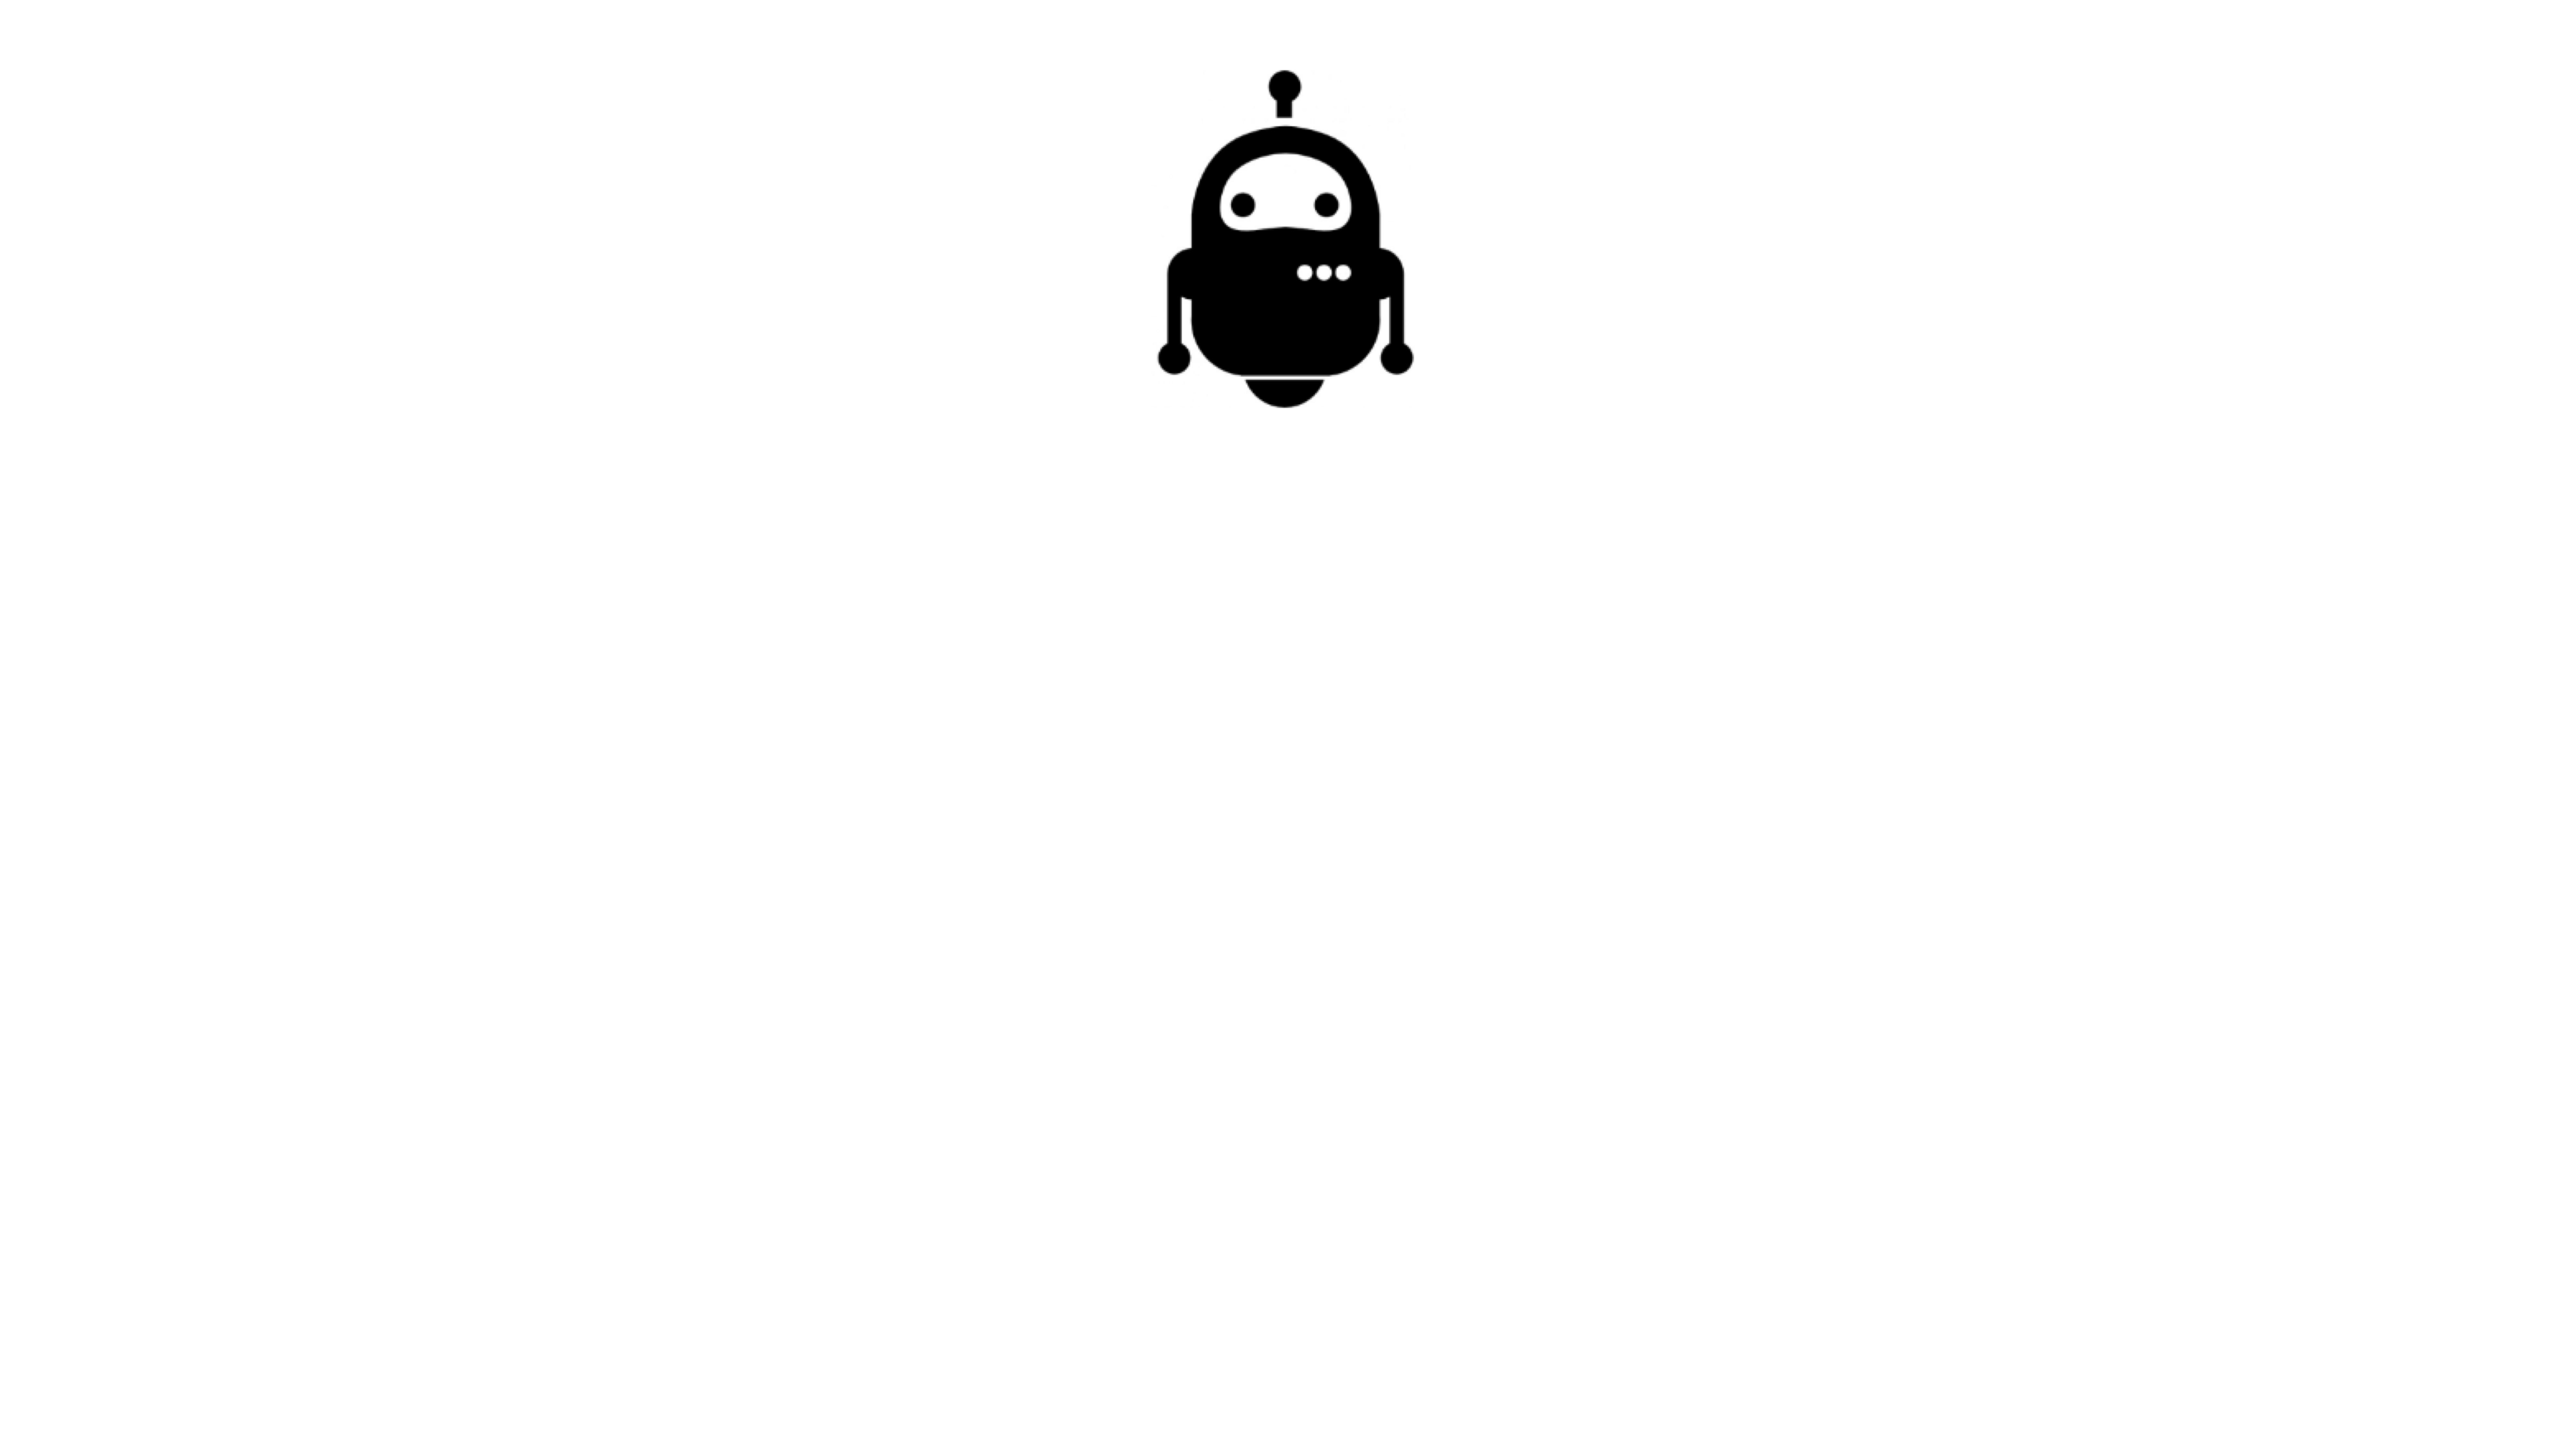
\includegraphics{figs/1_intro_rlmpc.png}
\end{center}

\begin{center}
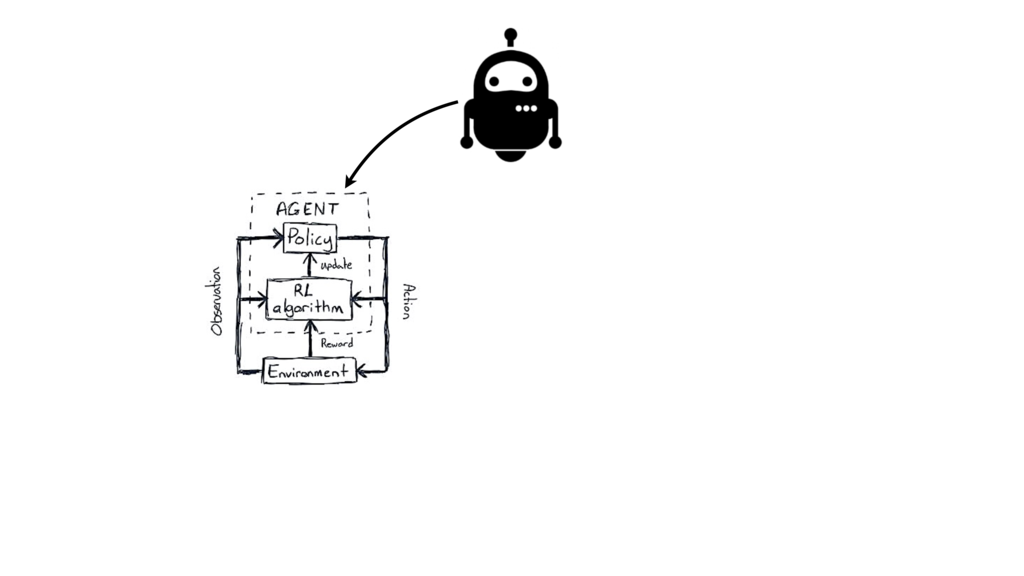
\includegraphics{figs/2_intro_rlmpc.png}
\end{center}

\begin{center}
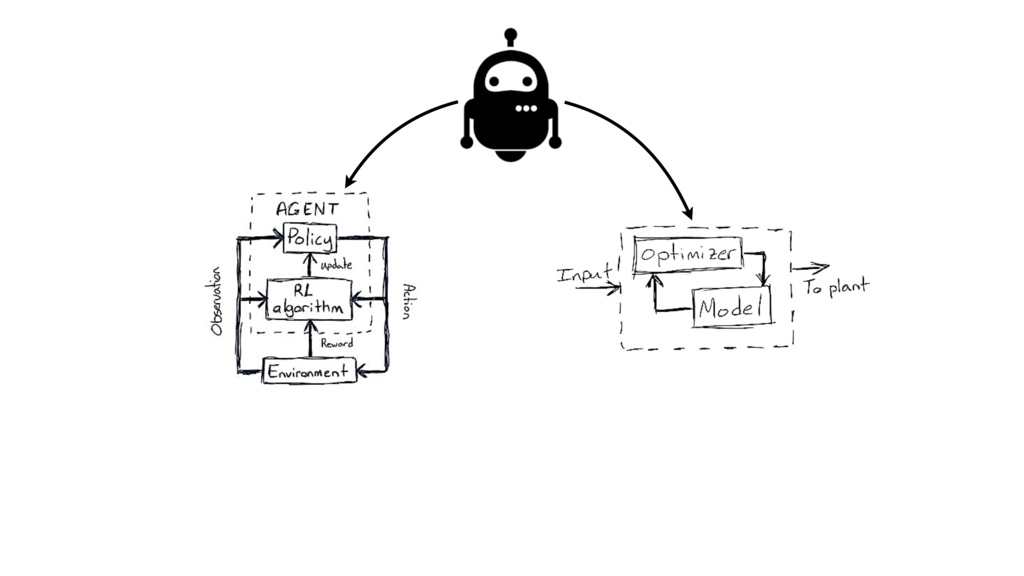
\includegraphics{figs/3_intro_rlmpc.png}
\end{center}

\begin{center}
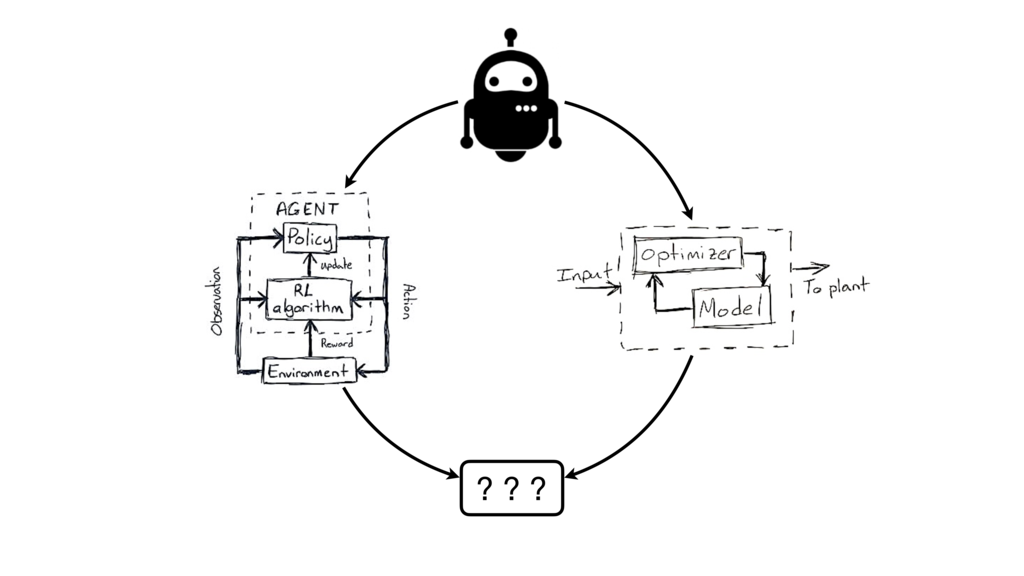
\includegraphics{figs/4_intro_rlmpc.png}
\end{center}

\marginnote{\begin{footnotesize}

\href{https://www.mathworks.com/solutions/control-systems/feedback-control-systems.html}{Sketches--Brian
Douglas}

\end{footnotesize}}

\subsection{}\label{section-1}

Day-to-day life depends on safely regulating a system around a constant
value:

\begin{enumerate}
\def\labelenumi{\arabic{enumi}.}
\tightlist
\item
  Cruise control
\item
  Temperature
\item
  Concentrations
\end{enumerate}

\begin{enumerate}
\def\labelenumi{\arabic{enumi}.}
\setcounter{enumi}{3}
\tightlist
\item
  Levels
\item
  Moisture
\item
  Etc\ldots{}
\end{enumerate}

\begin{center}

\includegraphics[width=\textwidth,height=1.5625in]{figs/sysid.png}
\end{center}

\subsection{}\label{section-2}

\begin{center}
\includegraphics{figs/1_mapofcontrol.png}
\end{center}

\begin{center}
\includegraphics{figs/2_mapofcontrol.png}
\end{center}

\subsection{Today}\label{today}

Combine reinforcement learning (RL) \& model predictive control (MPC)!

\begin{itemize}
\tightlist
\item
  RL, MPC, and some stuff in-between pertaining to process control
\item
  How to implement these ideas
\item
  Emphasis on intuition rather than rigor
\item
  Ask questions and be ready to discuss things with your neighbor
\end{itemize}

\begin{figure}[H]

{\centering 
\includegraphics{figs/qr-cheatsheet.png}

}

\caption{Cheat sheet!}

\end{figure}%

I hope this works for you!

\section{Reinforcement learning}\label{reinforcement-learning}

\subsection{Agents and environments}\label{agents-and-environments}

\subsection{Environment}\label{environment}

\begin{figure}

\begin{minipage}{0.23\linewidth}
Apply torque\end{minipage}%
%
\begin{minipage}{0.39\linewidth}
\begin{center}
\includegraphics[width=\textwidth,height=3.64583in]{figs/pendulum.gif}
\end{center}
\end{minipage}%
%
\begin{minipage}{0.39\linewidth}
Observe

\begin{itemize}
\tightlist
\item
  Angle
\item
  Angular velocity
\end{itemize}

\end{minipage}%

\end{figure}%

\subsection{Environment}\label{environment-1}

\(s_t\) -- state

\(a_t\) -- action

Actions and states lead to new states
\[s_{t+1} \sim p \left( s_{t+1} \middle| s_t, a_t \right)\]

\begin{center}
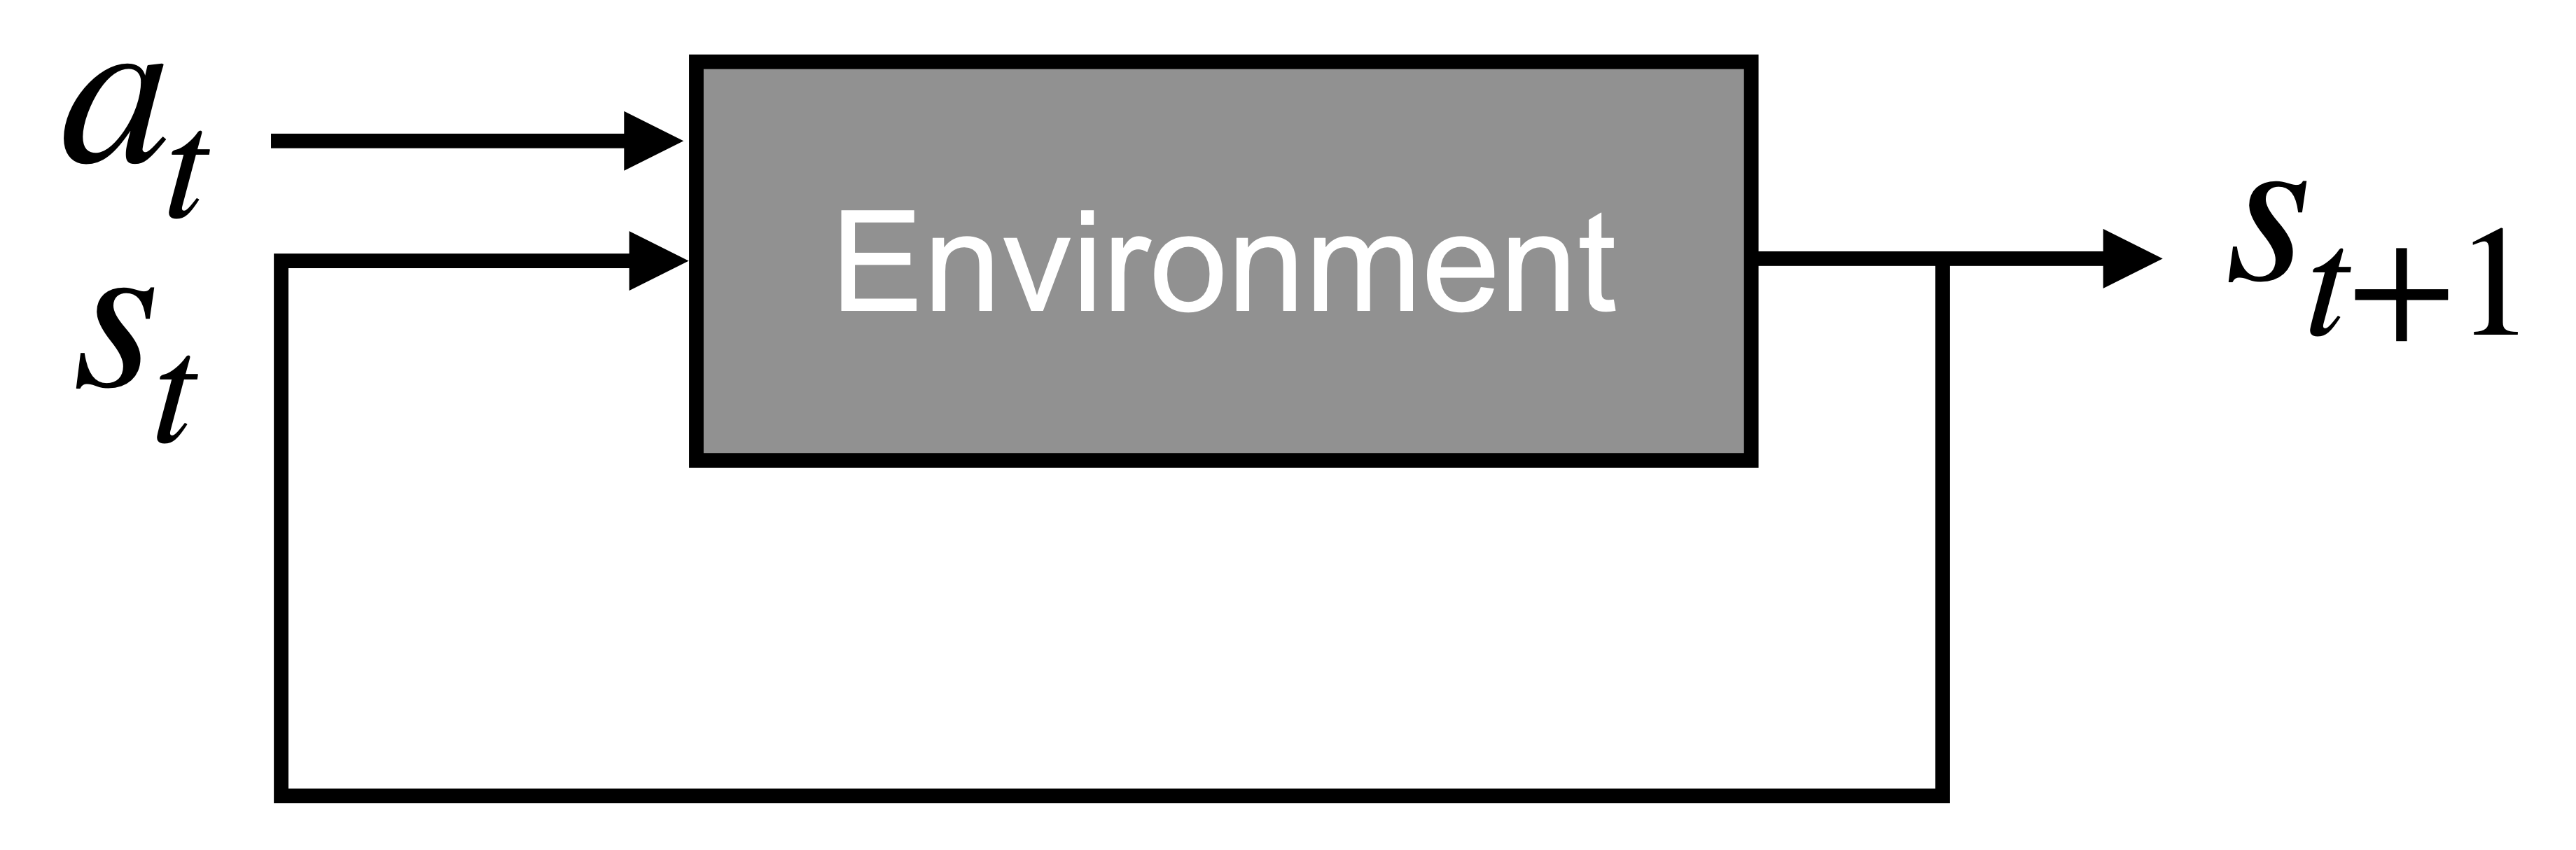
\includegraphics[width=\textwidth,height=2.08333in]{figs/mdp.png}
\end{center}

\subsection{Environment}\label{environment-2}

Continuing forever gives a trajectory
\[s_0, a_0, s_1, a_1, \ldots, s_{t}, a_{t}, s_{t+1}, \ldots\]

Most trajectories are ``bad''

We want a system that discovers ``good'' behavior in the environment

\begin{center}
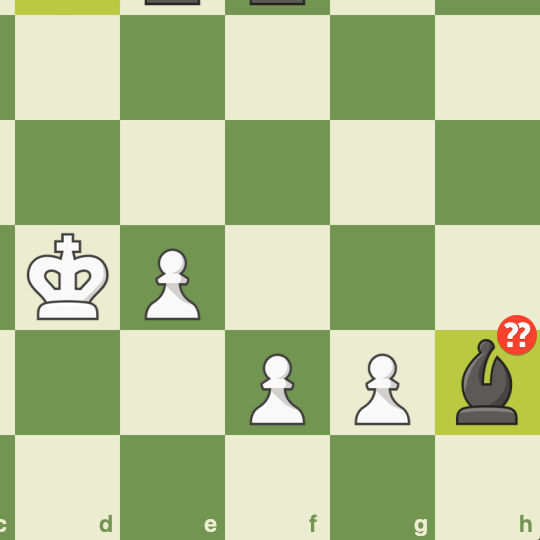
\includegraphics[width=\textwidth,height=2.08333in]{figs/blunder.png}
\end{center}

\subsection{Agent}\label{agent}

The agent is the learner:

\begin{itemize}
\tightlist
\item
  Decides which actions to take
\item
  Improves its behavior
\end{itemize}

\begin{center}
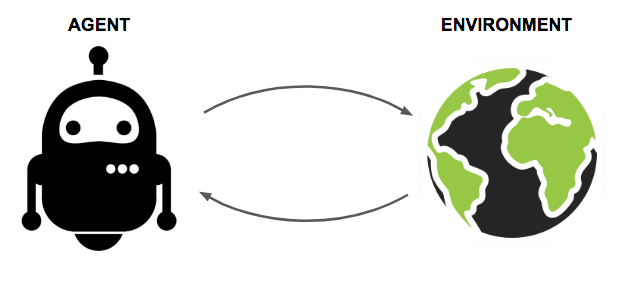
\includegraphics{figs/RL_illustration.png}
\end{center}

\marginnote{\begin{footnotesize}

Figure: L. Weng (2018)

\end{footnotesize}}

\subsection{Agent}\label{agent-1}

\textbf{Reward} guides learning:

\begin{itemize}
\tightlist
\item
  A scalar feedback signal
\item
  Indicates which states \& actions are good
\end{itemize}

\begin{center}
\includegraphics[width=\textwidth,height=2.60417in]{figs/RLSutton.png}
\end{center}

\marginnote{\begin{footnotesize}

Figure: Sutton and Barto (2018)

\end{footnotesize}}

\subsection{What are we really trying to
solve?}\label{what-are-we-really-trying-to-solve}

\subsection{}\label{section-3}

The agent-environment interface yields the trajectory
\[s_0, a_0, r_0, s_1, a_1, r_1 \ldots, s_{t}, a_{t}, r_{t}, s_{t+1}, \ldots\]

States governed by
\[s_{t+1} \sim p \left( s_{t+1} \middle| s_t, a_t \right)\] Agent
chooses actions from a \textbf{policy}
\[a_t \sim \pi\left( a_t \middle| s_t \right)\] Rewards assigned by a
function \[r_t = r(s_t, a_t)\]

\subsection{The space of policies is
vast}\label{the-space-of-policies-is-vast}

\begin{itemize}
\tightlist
\item
  Completely random
\item
  An industrial control module
\item
  Neural network
\end{itemize}

\begin{center}
\includegraphics[width=\textwidth,height=1.97917in]{figs/gritty.gif}
\end{center}

\begin{center}
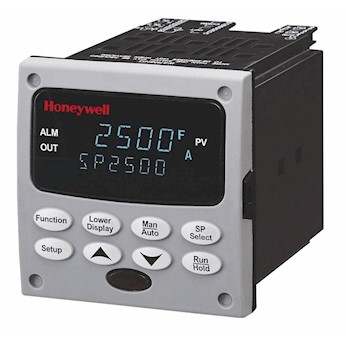
\includegraphics[width=\textwidth,height=2.1875in]{figs/Honey_UDC.jpg}
\end{center}

\begin{center}
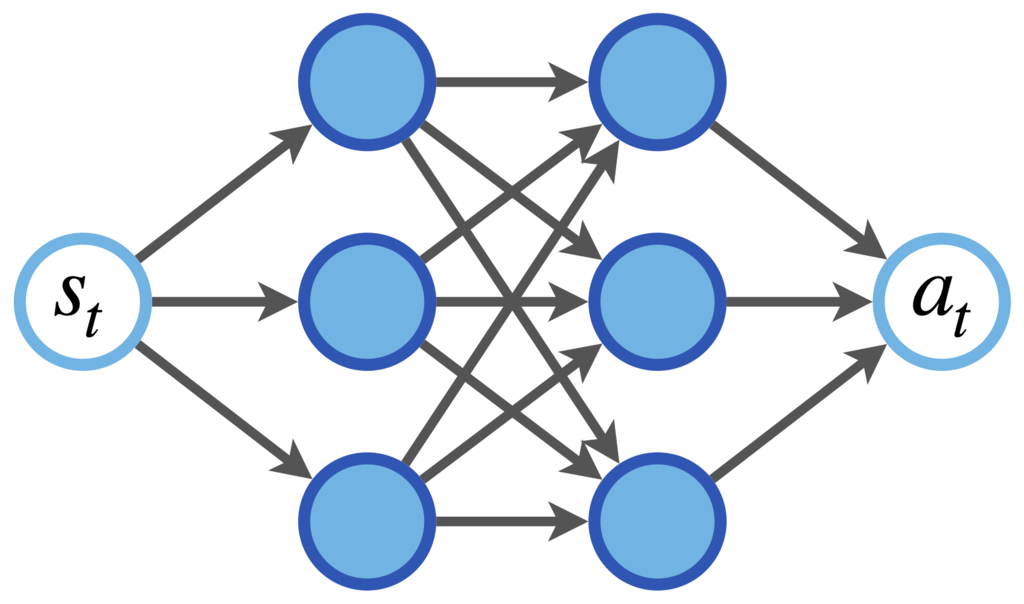
\includegraphics[width=\textwidth,height=2.39583in]{figs/nn.png}
\end{center}

\subsection{Restricting the policy space is
practical}\label{restricting-the-policy-space-is-practical}

\begin{figure}

\begin{minipage}{0.20\linewidth}
\begin{center}
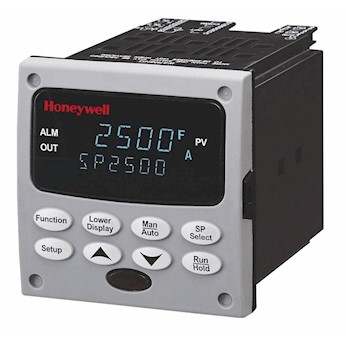
\includegraphics[width=\textwidth,height=1.5625in]{figs/Honey_UDC.jpg}
\end{center}
\end{minipage}%
%
\begin{minipage}{0.80\linewidth}
\begin{center}
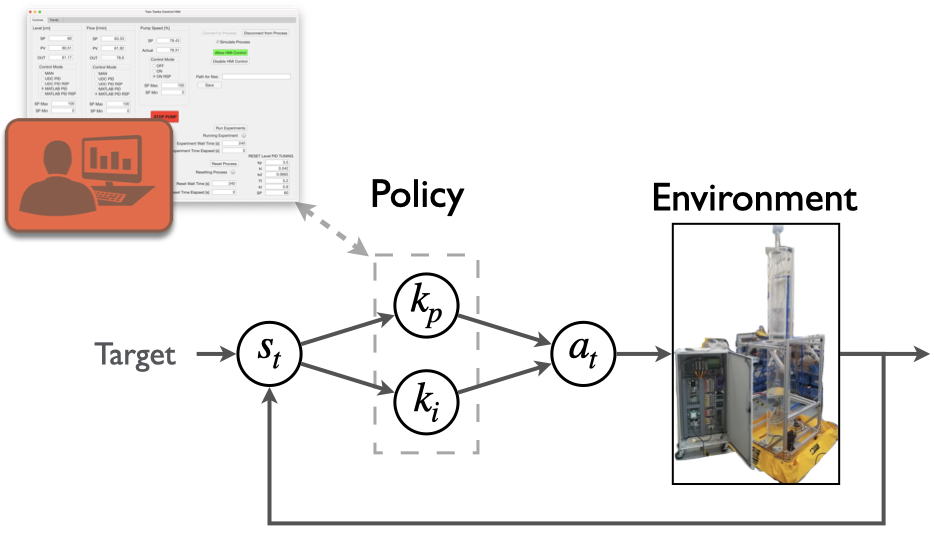
\includegraphics[width=\textwidth,height=3.38542in]{figs/rl-pid.png}
\end{center}
\end{minipage}%

\end{figure}%

\marginnote{\begin{footnotesize}

See Lawrence et al. (2022)

\end{footnotesize}}

\subsection{We want the ``best'' policy!}\label{we-want-the-best-policy}

\begin{itemize}
\tightlist
\item
  Take \(a \in \text{argmax}_{a} \left\{ r(s,a) \right\}\)?
\end{itemize}

\(\rightarrow\) too shortsighted

\begin{itemize}
\tightlist
\item
  Maximize \(r_0 + r_1 + r_2 + \ldots\)?
\end{itemize}

\(\rightarrow\) might diverge

Consider the discounted \textbf{return}
\[G_t = r_t + \gamma r_{t+1} + \gamma^2 r_{t+2} + \ldots\] where
\(\gamma \in [0,1]\)

\subsection{}\label{section-4}

\begin{itemize}
\tightlist
\item
  Typically, \(\gamma \in (0,1)\)
\item
  Assume \(r\) is bounded by \(\bar{r}\)
\end{itemize}

Return is bounded across all possible trajectories
\[\lvert G_t \rvert \leq \frac{\bar{r}}{1 - \gamma}\]

\begin{center}
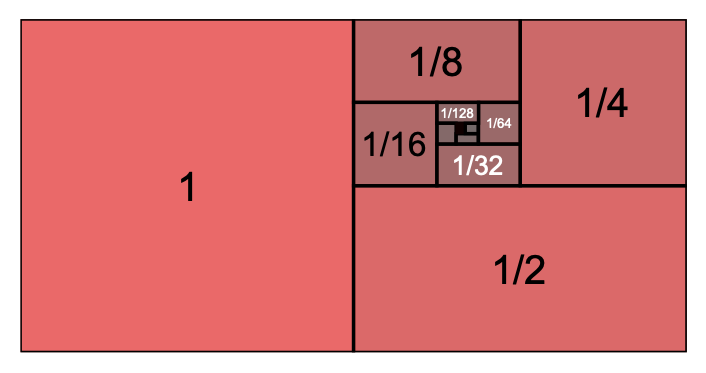
\includegraphics[width=\textwidth,height=2.08333in]{figs/geometric.png}
\end{center}

\marginnote{\begin{footnotesize}

\href{https://en.wikipedia.org/wiki/Geometric_series}{Geometric series
(Wikipedia)}

\end{footnotesize}}

\subsection{The reinforcement learning
problem}\label{the-reinforcement-learning-problem}

\[ \text{maximize} \quad J(\pi) = \mathbb{E}_{\pi}\left[ \sum_{t=0}^{\infty} \gamma^{t}r(s_t,a_t) \right]\]

\subsection{The reinforcement learning
problem}\label{the-reinforcement-learning-problem-1}

\[ \text{maximize} \quad J(\pi) = \mathbb{E}_{\pi}\left[ \sum_{t=0}^{\infty} \gamma^{t}r(s_t,a_t) \right]\]

Why is this hard/impossible?

\begin{itemize}
\tightlist
\item
  Infinite horizon
\item
  Search space
\item
  Randomness
\item
  No system description
\end{itemize}

\subsection{Wishful thinking}\label{wishful-thinking}

\subsection{}\label{section-5}

What if we had an optimal trajectory?
\[s_0^\star, a_0^\star, r_0^\star, s_1^\star, a_1^\star, r_1^\star \ldots, s_{t}^\star, a_{t}^\star, r_{t}^\star, s_{t+1}^\star, \ldots\]

\begin{figure}

\begin{minipage}{0.67\linewidth}
Then the trajectory starting at \(s_t^\star\) should still be optimal
\[s_{t}^\star, a_{t}^\star, r_{t}^\star, s_{t+1}^\star, \ldots\]\end{minipage}%
%
\begin{minipage}{0.33\linewidth}
\begin{center}
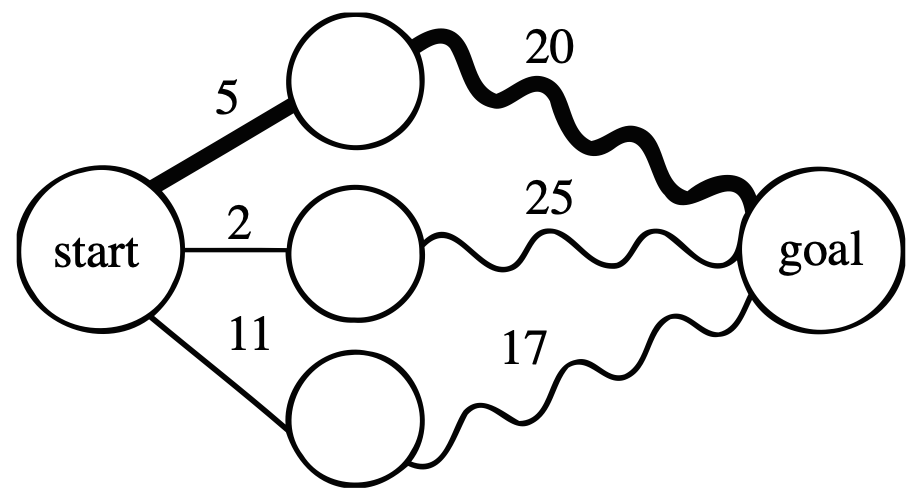
\includegraphics{figs/subpath.png}
\end{center}
\end{minipage}%

\end{figure}%

\marginnote{\begin{footnotesize}

\href{https://en.wikipedia.org/wiki/Optimal_substructure}{Optimal
substructure (Wikipedia)}

\end{footnotesize}}

\subsection{Chess example}\label{chess-example}

(placeholder -- think about planning backwards from checkmate)

\subsection{}\label{section-6}

\begin{itemize}
\tightlist
\item
  Define the \textbf{state-action value} to be
  \[Q^\pi (s,a) = \mathbb{E}_{\pi}\left[ \sum_{t=0}^{\infty} \gamma^{t}r(s_t,a_t) | s_0 = s, a_0 = a \right]\]
\item
  Similarly, the (state) \textbf{value} averages over the policy:
  \begin{align}
  V^\pi (s) &= \mathbb{E}_{\pi}\left[ \sum_{t=0}^{\infty} \gamma^{t}r(s_t,a_t) | s_0 = s \right]\\
  &= \mathbb{E}_{a \sim \pi(a | s)}\left[ Q^\pi (s,a) \right]
  \end{align}
\end{itemize}

\subsection{Abstracting the objective through value
functions}\label{abstracting-the-objective-through-value-functions}

\[J(\pi) = \mathbb{E}_{s_0 \sim p(s_0)}\left[ V^\pi (s_0) \right]\]

\subsection{What's the big deal with these magical
functions?}\label{whats-the-big-deal-with-these-magical-functions}

Observe \begin{align}
G_t &= r_t + \gamma r_{t+1} + \gamma^2 r_{t+2} + \ldots \\
&= r_t + \gamma \left( r_{t+1} + \gamma r_{t+2} + \ldots \right) \\
&= r_t + \gamma G_{t+1}
\end{align}

Compresses an infinite number of actions into a simple scalar recursion!

\subsection{What's the big deal with these magical
functions?}\label{whats-the-big-deal-with-these-magical-functions-1}

Averaging\ldots{}

\begin{align}
V^\pi (s) &= \mathbb{E}_{\pi} \left[ G_t \middle| s_t = s \right] \\
&= \mathbb{E}_{\pi} \left[ r_t + \gamma G_{t+1} \middle| s_t = s \right] \\
&= \mathbb{E}_{a \sim \pi(a | s)} \left[ r(s,a) + \gamma \mathbb{E}_{s' \sim p(s' | s, a)} \left[ V^\pi (s') \right]\right]
\end{align}

\subsection{What's the big deal with these magical
functions?}\label{whats-the-big-deal-with-these-magical-functions-2}

Similarly for \(Q^\pi\)\ldots{}

\begin{align}
Q^\pi (s,a) &= r(s,a) + \gamma \mathbb{E}_{s' \sim p(s' | s, a)}\left[ V^\pi (s') \right]\\
&= r(s,a) + \gamma \mathbb{E}_{s' \sim p(s' | s, a), a' \sim \pi(a' | s')}\left[ Q^\pi (s',a') \right]
\end{align}

\subsection{What's the big deal with these magical
functions?}\label{whats-the-big-deal-with-these-magical-functions-3}

These are the \textbf{Bellman equations} for \(V\) and \(Q\)

\begin{align}
\bbox[#d8d0ff,2pt]{V(s)} &= \mathbb{E}\left[ r(s,a) + \gamma \bbox[#d8d0ff,2pt]{V(s')} \right] \\
\bbox[#e0ffd0,2pt]{Q(s,a)} &= r(s,a) + \gamma \mathbb{E}\left[ \bbox[#e0ffd0,2pt]{Q(s',a')} \right]
\end{align}

Bellman equation holds for any policy!

\subsection{Bellman optimality
equation}\label{bellman-optimality-equation}

An optimal policy \(\pi^\star\) solves the following:

\begin{figure}

\begin{minipage}{0.50\linewidth}
\[V^\star (s) = \max_{\pi} V^\pi (s)\]\end{minipage}%
%
\begin{minipage}{0.50\linewidth}
\[Q^\star (s,a) = \max_{\pi} Q^\pi (s,a)\]\end{minipage}%

\end{figure}%

We don't actually have \(\pi^\star\), but it's fun to imagine\ldots{}

\subsection{Bellman optimality
equation}\label{bellman-optimality-equation-1}

Given \(V^\star\)\ldots{}

\begin{align}
V^\star (s) &= \mathbb{E}_{a \sim \pi^\star (a | s)} \left[ r(s,a) + \gamma \mathbb{E}_{s' \sim p(s' | s, a)} \left[ V^\star (s') \right]\right]\\
&= \max_{a}\left\{ r(s,a) + \gamma \mathbb{E}_{s' \sim p(s' | s, a)} \left[ V^\star (s') \right] \right\}
\end{align}

\begin{center}
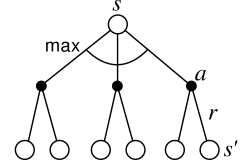
\includegraphics[width=\textwidth,height=1.5625in]{figs/v_backup.png}
\end{center}

One-step planning is long-term optimal

\subsection{Bellman optimality
equation}\label{bellman-optimality-equation-2}

Given \(Q^\star\)\ldots{} \[V^\star (s) = \max_{a} Q^\star (s,a)\]

\ldots Even easier!

Learn \(Q^\star\) and then maximize it!

\subsection{Evaluate, improve,
repeat\ldots{}}\label{evaluate-improve-repeat}

\subsection{}\label{section-7}

Like \(V^\star\), \(Q^\star\) satisfies a neat optimality condition:

\begin{align}
\bbox[#e0ffd0,2pt]{Q^\star} (s,a) &= r(s,a) + \gamma \mathbb{E}_{s' \sim p(s' | s, a), a' \sim \pi^\star (a' | s')}\left[ Q^\star (s',a') \right] \\
&= r(s,a) + \gamma  \mathbb{E}_{s' \sim p(s' | s, a)}\left[ \max_{a'} \bbox[#e0ffd0,2pt]{Q^\star} (s',a') \right]
\end{align}

``Plug this magical function \(Q^\star\) into the RHS produces the same
function''

\subsection{Fixed-point iteration}\label{fixed-point-iteration}

Iterating \(q^{k+1} = B(q^k)\) \textbf{may} converge to some \(q\) where
\(q = B(q)\)

\begin{center}
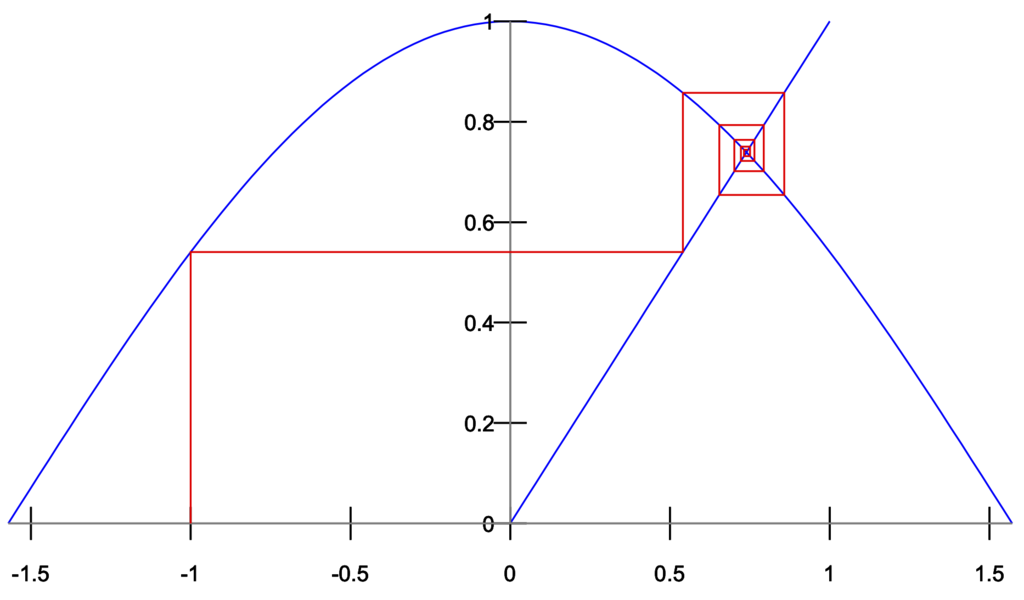
\includegraphics[width=\textwidth,height=3.64583in]{figs/fixedpoint.png}
\end{center}

\subsection{}\label{section-8}

\begin{itemize}
\item
  Let's just take the operator
  \[B(Q^\pi) = r(s,a) + \gamma  \mathbb{E}_{s' \sim p(s' | s, a)}\left[ \max_{a'} Q^\pi (s',a') \right]\]
  and apply fixed-point iteration!
\item
  The RHS is an \textbf{idealized} update scheme and key source of
  inspiration
\end{itemize}

\subsection{Fixed-point aspirations}\label{fixed-point-aspirations}

If we have a policy \(\pi\) and some oracle that tells us \(Q^\pi\),
take \begin{align}
\pi^{+}(s) &= \text{arg}\max\limits_{a} Q^\pi (s,a) \\
&= \text{arg}\max\limits_{a} \left\{ r(s,a) + \gamma \mathbb{E}_{s' \sim p(s' | s, a)} \left[ V^\pi  (s') \right] \right\}
\end{align}

Then \(\pi^{+}\) is at least as good as \(\pi\)! That is,
\(Q^{+} = B(Q^\pi) \geq Q^\pi\).

When improvement is no longer possible, we have \[
\pi^\star (s) = \arg \max_{a} Q^\star (s,a).
\]

\subsection{}\label{section-9}

There are many ways to proceed: Policy iteration, value iteration, and
we haven't even mentioned policy evaluation. We're focusing on
high-level ideas and avoiding introducing jargon, so see Sutton and
Barto (2018) for a full treatment.

\subsection{}\label{section-10}

\[\pi^{+}(s) = \bbox[#DCD0FF,2pt]{\text{arg}\max\limits_{a}} \left\{ r(s,a) + \gamma \bbox[#FF9999,2pt]{\mathbb{E}} \left[ \bbox[#AAF0D1,2pt]{V^\pi (s')} \right] \right\}\]

\subsection{Three important
approximations}\label{three-important-approximations}

\begin{center}
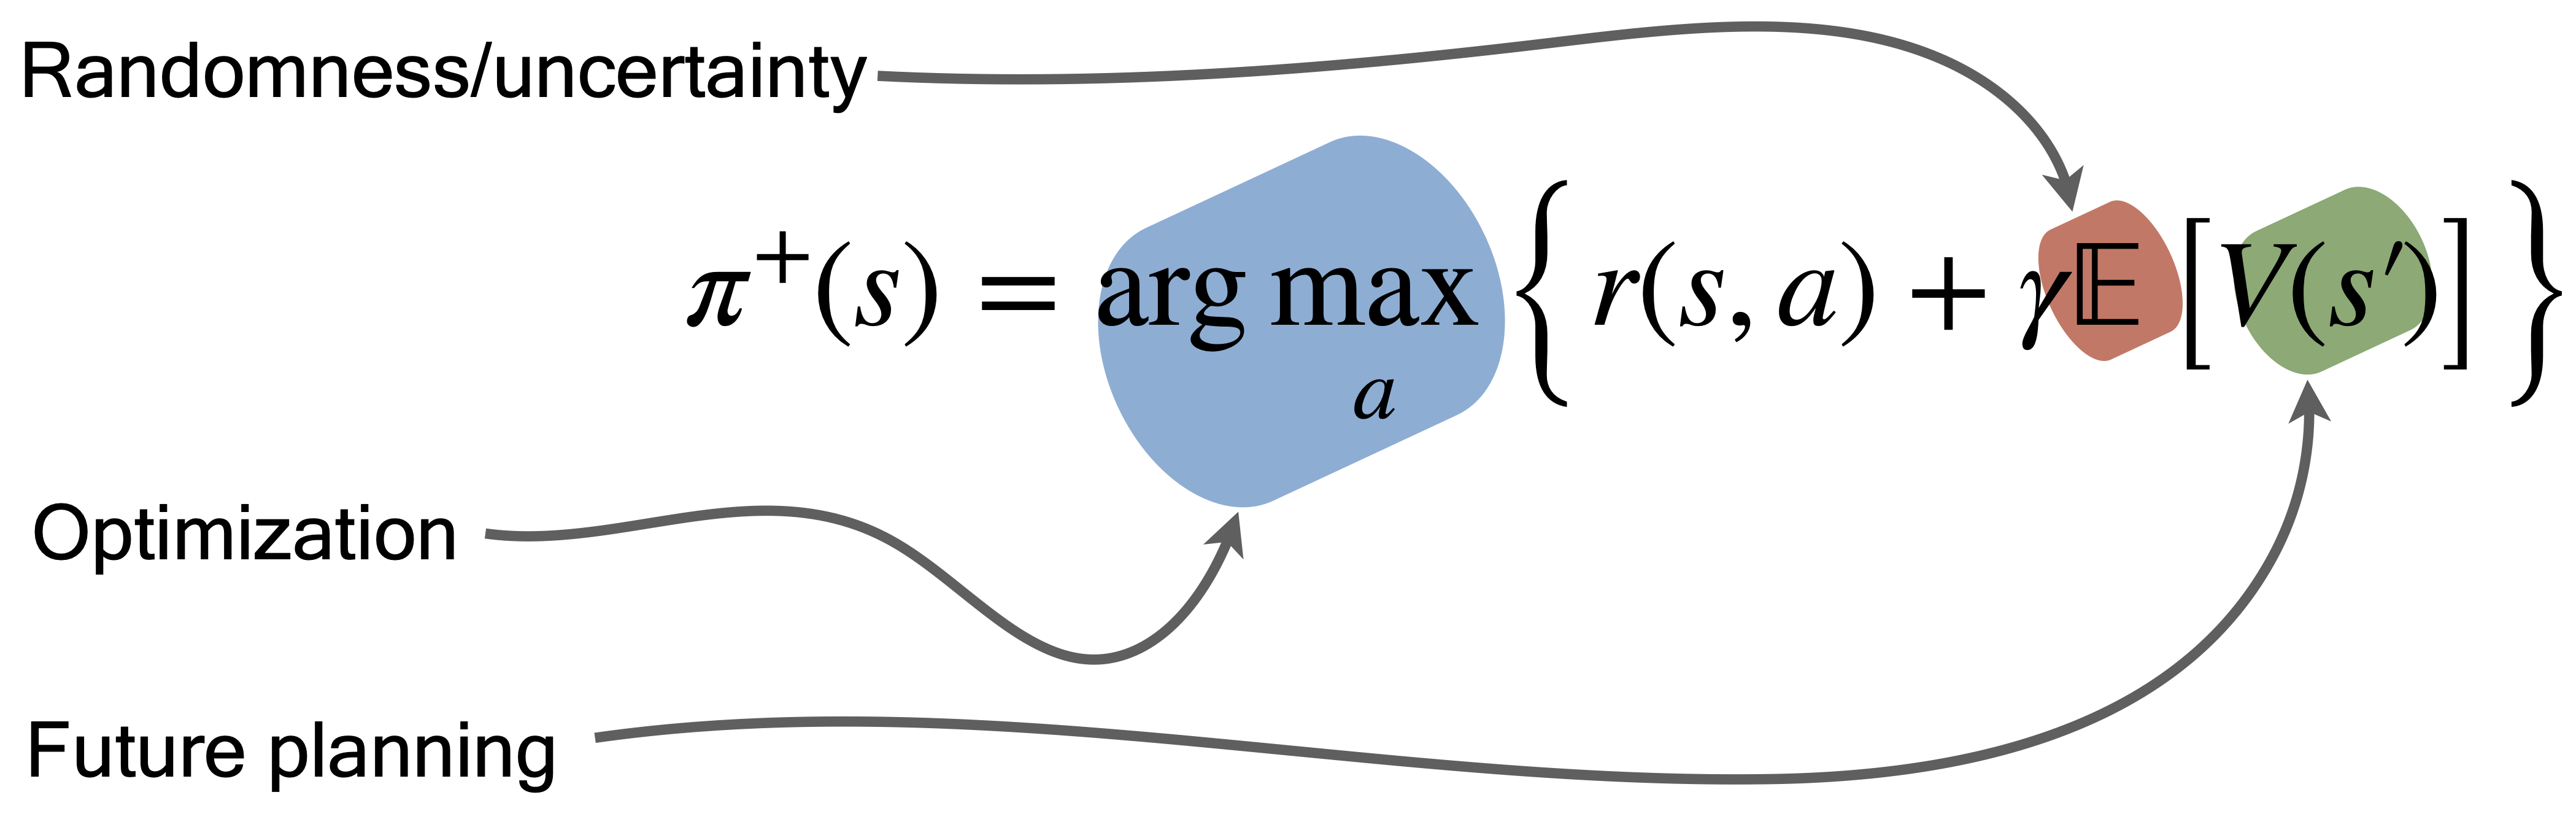
\includegraphics{figs/pi_update.png}
\end{center}

\marginnote{\begin{footnotesize}

See works by \href{https://www.mit.edu/~dimitrib/home.html}{Dimitri
Bertsekas} (most recently Bertsekas (2023))

\end{footnotesize}}

\subsection{}\label{section-11}

\begin{figure}

\begin{minipage}{\linewidth}
To move things along we will work through some examples instead of
focusing on the minutiae of common RL algorithms\end{minipage}%
\newline
\begin{minipage}{\linewidth}
\begin{center}
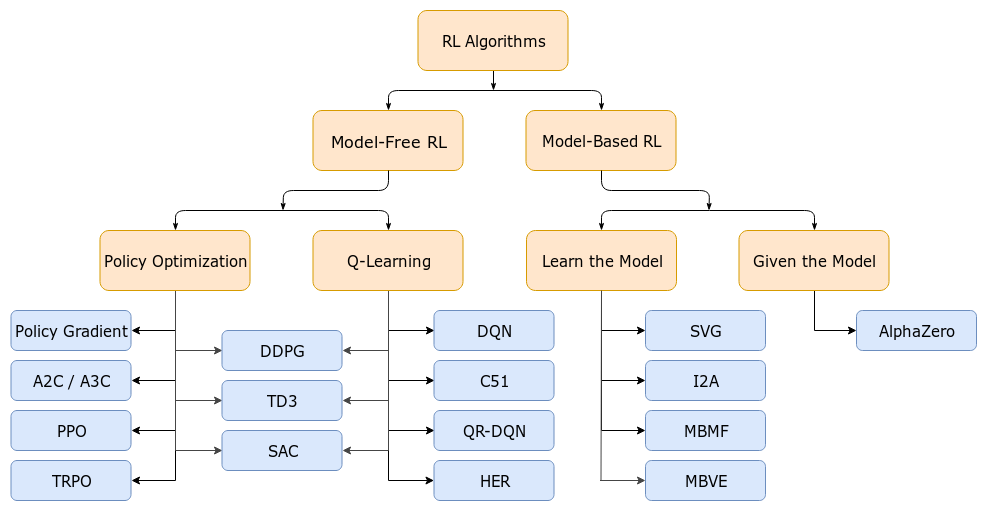
\includegraphics[width=\textwidth,height=4.16667in]{figs/rl_algs.png}
\end{center}
\end{minipage}%

\end{figure}%

\marginnote{\begin{footnotesize}

Figure:
\href{https://spinningup.openai.com/en/latest/spinningup/rl_intro2.html}{Spinning
Up}

\end{footnotesize}}

\section{Examples}\label{examples}

\subsection{Learning to balance}\label{learning-to-balance}

\subsection{Cartpole}\label{cartpole}

\begin{figure}

\begin{minipage}{0.65\linewidth}
\includegraphics[width=\textwidth,height=0.9\textheight]{figs/cart_pole.gif}\end{minipage}%
%
\begin{minipage}{0.35\linewidth}
\textbf{Don't fall!}\end{minipage}%

\end{figure}%

\subsection{Deep Q-networks (DQNs)}\label{deep-q-networks-dqns}

For a \textbf{finite} set of actions, define the neural network
\[\text{DQN}(s) =
\begin{bmatrix}
q_1 \\
\vdots \\
q_d
\end{bmatrix}\] where each \(q_i\) is an approximation of
\(Q^\pi (s,a_i)\)

\marginnote{\begin{footnotesize}

Mnih et al. (2013)

\end{footnotesize}}

\subsection{}\label{section-12}

Optimization is trivial: \begin{align}
\pi(s) &= \arg\max \text{DQN}(s) \\
&= \arg\max\left\{ q_1, \ldots, q_d \right\} \\
&\approx \arg\max_{a} Q^\pi (s,a_i)
\end{align}

\subsection{}\label{section-13}

\begin{figure}

\begin{minipage}{\linewidth}
\begin{center}
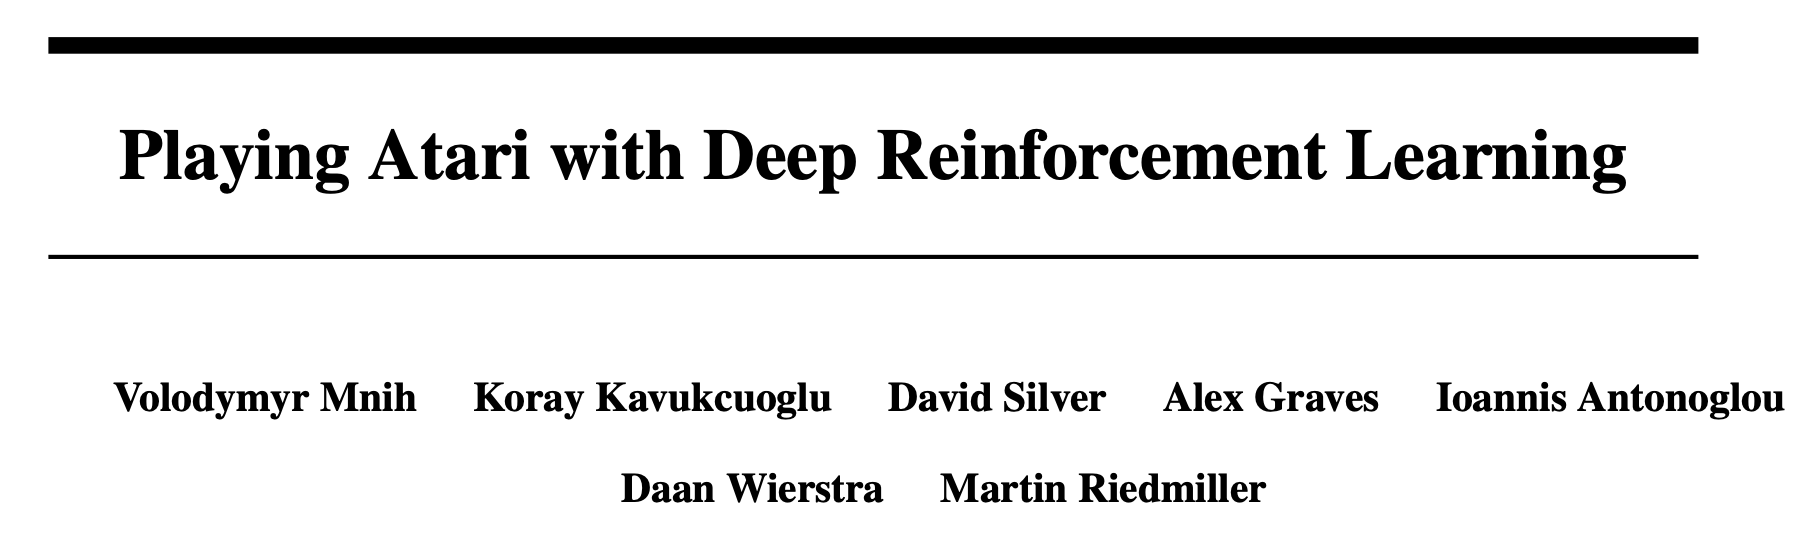
\includegraphics[width=\textwidth,height=1.5625in]{figs/mnih_atari.png}
\end{center}
\end{minipage}%
\newline
\begin{minipage}{\linewidth}
\begin{center}
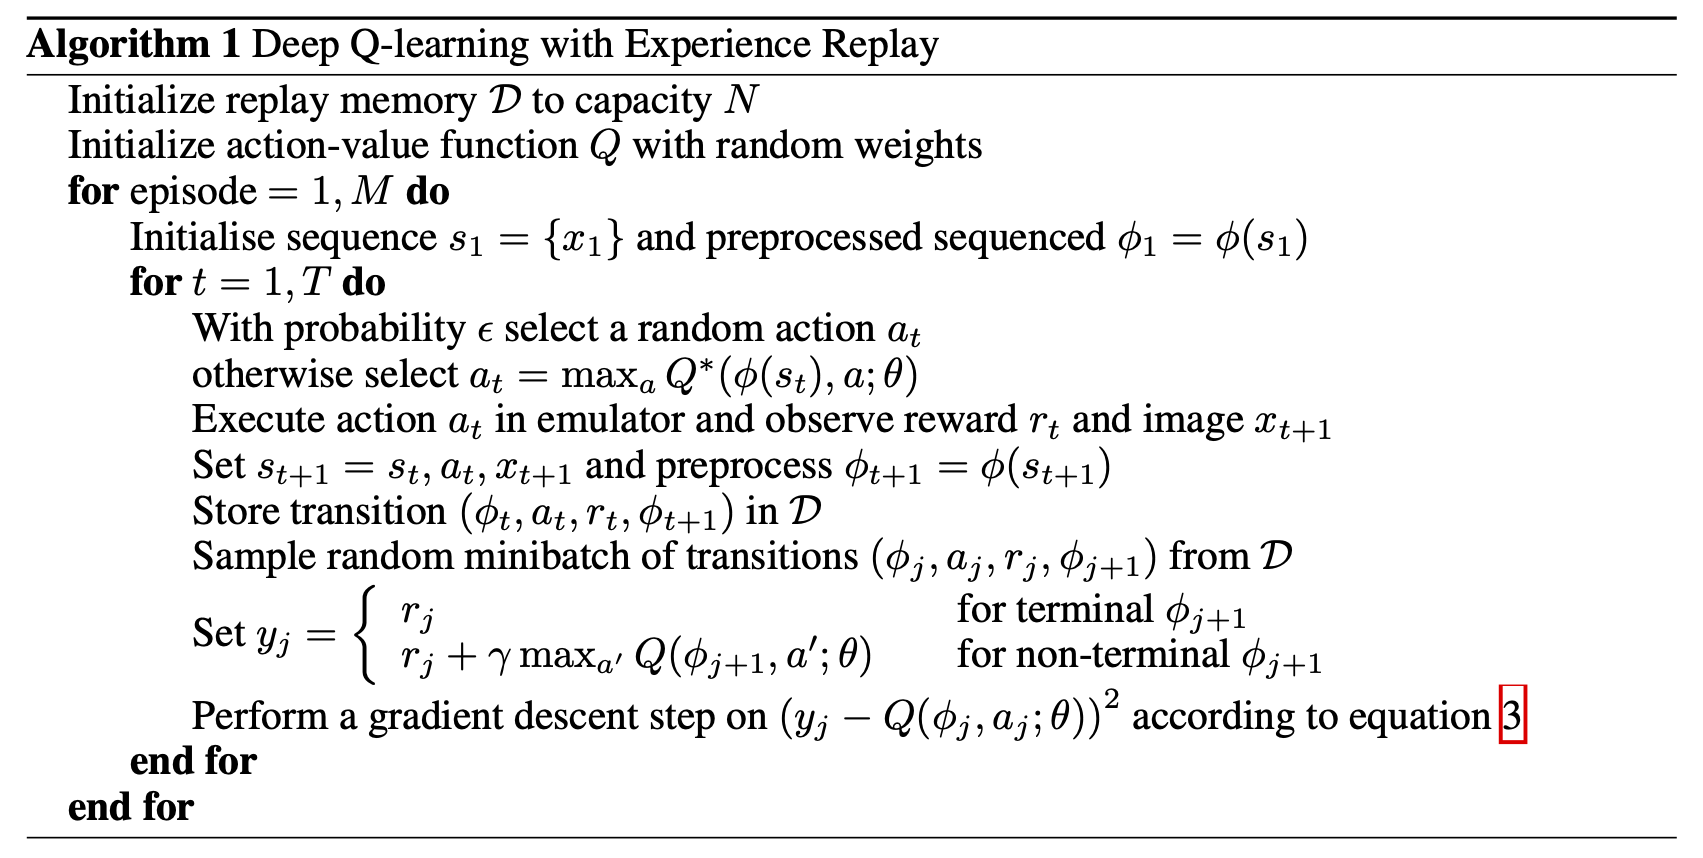
\includegraphics[width=\textwidth,height=3.125in]{figs/mnih_algo.png}
\end{center}
\end{minipage}%

\end{figure}%

\marginnote{\begin{footnotesize}

Equation 3: Approximately respect the Bellman equation
\([q_1, \ldots, q_d] \approx r(s,a) + \gamma \max\{ q_1', \ldots q_d'\}\)

\end{footnotesize}}

\subsection{}\label{section-14}

\begin{figure}

\begin{minipage}{0.50\linewidth}

\begin{figure}[H]

{\centering \includegraphics[width=3.125in,height=\textheight]{videos/dqn/episode-398.gif}

}

\subcaption{Initial}

\end{figure}%

\end{minipage}%
%
\begin{minipage}{0.50\linewidth}

\begin{figure}[H]

{\centering \includegraphics[width=3.125in,height=\textheight]{videos/dqn/episode-6965.gif}

}

\subcaption{After some time\ldots{}}

\end{figure}%

\end{minipage}%
\newline
\begin{minipage}{0.50\linewidth}

\begin{figure}[H]

{\centering \includegraphics[width=3.125in,height=\textheight]{videos/dqn/episode-8159.gif}

}

\subcaption{Almost there\ldots{}}

\end{figure}%

\end{minipage}%
%
\begin{minipage}{0.50\linewidth}

\begin{figure}[H]

{\centering \includegraphics[width=3.125in,height=\textheight]{videos/dqn/episode-8358.gif}

}

\subcaption{Final}

\end{figure}%

\end{minipage}%

\end{figure}%

\subsection{Acrobot}\label{acrobot}

\begin{figure}

\begin{minipage}{0.65\linewidth}
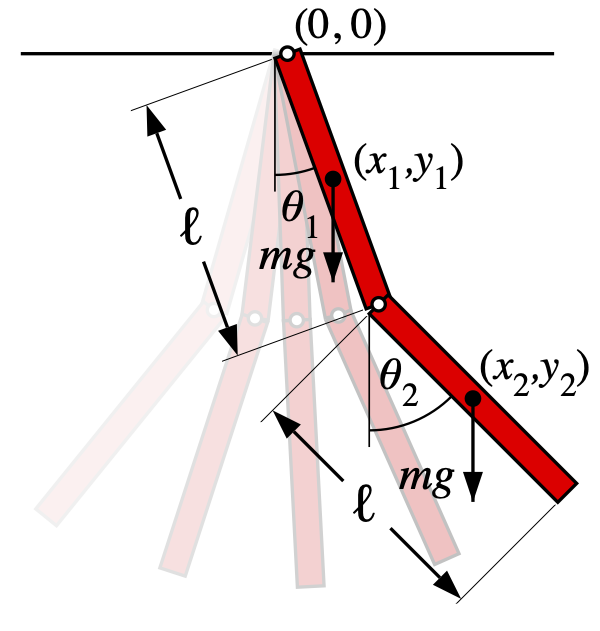
\includegraphics{figs/acrobot.gif}\end{minipage}%
%
\begin{minipage}{0.35\linewidth}
\textbf{Touch the line!}\end{minipage}%

\end{figure}%

\subsection{Acrobot}\label{acrobot-1}

\begin{figure}

\begin{minipage}{0.65\linewidth}
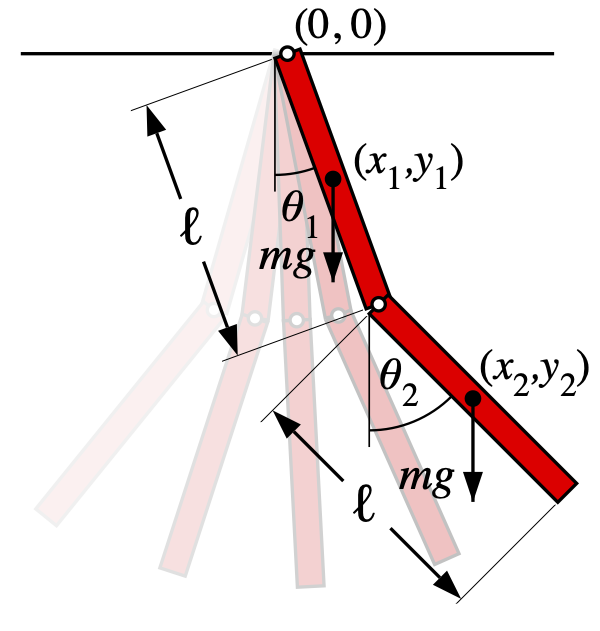
\includegraphics{figs/acrobot.gif}\end{minipage}%
%
\begin{minipage}{0.35\linewidth}
\st{\textbf{Touch the line!}}\textbf{Stay above the
line!}\end{minipage}%

\end{figure}%

\subsection{}\label{section-15}

Applying DQN\ldots{}

\begin{figure}

\begin{minipage}{0.50\linewidth}

\begin{figure}[H]

{\centering \includegraphics[width=2.08333in,height=\textheight]{videos/dqn/acrobot-dqn__0__episode-0.mp4}

}

\subcaption{Initial}

\end{figure}%

\end{minipage}%
%
\begin{minipage}{0.50\linewidth}

\begin{figure}[H]

{\centering \includegraphics[width=2.08333in,height=\textheight]{videos/dqn/acrobot-dqn__0__episode-796.mp4}

}

\subcaption{After some time\ldots{}}

\end{figure}%

\end{minipage}%
\newline
\begin{minipage}{0.50\linewidth}

\begin{figure}[H]

{\centering \includegraphics[width=2.08333in,height=\textheight]{videos/dqn/acrobot-dqn__0__episode-1592.mp4}

}

\subcaption{Almost there\ldots{}}

\end{figure}%

\end{minipage}%
%
\begin{minipage}{0.50\linewidth}

\begin{figure}[H]

{\centering \includegraphics[width=2.08333in,height=\textheight]{videos/dqn/acrobot-dqn__0__episode-1990.mp4}

}

\subcaption{Final}

\end{figure}%

\end{minipage}%

\end{figure}%

\marginnote{\begin{footnotesize}

Standing upright would be better than all of these\ldots{}

\end{footnotesize}}

\subsection{Finer control requires continuous
actions}\label{finer-control-requires-continuous-actions}

What we want: \[
\pi^\star (s) = \arg \max_{a} Q^\star (s,a)
\]

What DQN delivers:

\begin{align}
\pi(s) &= \arg \max \left\{ q_1, \ldots, q_d \right\} \\
&\approx \arg \max \left\{ Q^\star(s, a_1), \ldots, Q^\star(s, a_d)\right\}
\end{align}

\subsection{Finer control requires continuous
actions}\label{finer-control-requires-continuous-actions-1}

Consider two separate networks:

\begin{itemize}
\tightlist
\item
  Policy \(\pi_{\theta}\) (aka ``actor'')
\item
  \(Q\)-network \(Q_\varphi\) (aka ``critic'')
\end{itemize}

Idea: Use \(Q_\varphi\) as a loss function for \(\pi_{\theta}\):
\[\text{maximize}_{\theta} \quad \mathbb{E} \left[ Q_\varphi(s, \pi_\theta (s)) \right]\]

\subsection{}\label{section-16}

Then \[\max_{a} Q^\pi (s,a) \approx Q_\varphi (s, \pi_{\theta} (s))\]

An easy-to-evaluate approximation of the argmax operation!

\subsection{Disclaimer}\label{disclaimer}

This doesn't actually work.

See the DDPG, TD3, SAC papers for all the tricks/hacks that make this
idea work.

\begin{itemize}
\tightlist
\item
  Replay buffers
\item
  Target networks
\item
  Exploration / exploitation
\end{itemize}

\begin{itemize}
\tightlist
\item
  Double \(Q\)-learning
\item
  Delayed updates
\item
  Smoothing
\end{itemize}

\marginnote{\begin{footnotesize}

DDPG (Lillicrap et al. 2015), TD3 (Fujimoto, van Hoof, and Meger
2018-07-10/2018-07-15), SAC (Haarnoja et al. 2019)

\end{footnotesize}}

\subsection{Acrobot cont'd}\label{acrobot-contd}

Let's assume we have some RL oracle:

\emph{Given an environment and sufficiently powerful networks, it does a
reasonable job at solving the principal RL problem}

We isolate two components:

\begin{itemize}
\tightlist
\item
  Reward function
\item
  Discount factor \(\gamma\)
\end{itemize}

\subsection{Todo: Try to formulate a reward
function}\label{todo-try-to-formulate-a-reward-function}

\begin{figure}

\begin{minipage}{0.50\linewidth}
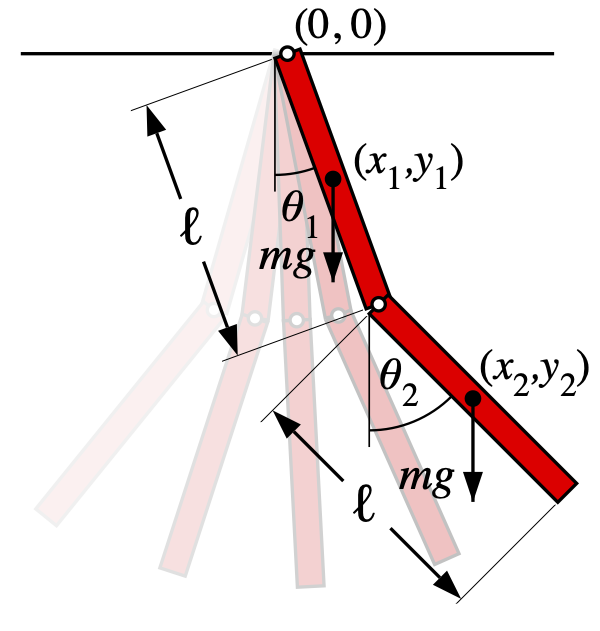
\includegraphics[width=\textwidth,height=3.125in]{figs/acrobot.png}\end{minipage}%
%
\begin{minipage}{0.50\linewidth}
\includegraphics[width=\textwidth,height=3.125in]{figs/dp.gif}\end{minipage}%

\end{figure}%

\marginnote{\begin{footnotesize}

\href{https://en.wikipedia.org/wiki/Double_pendulum}{Double pendulum
{[}Wikipedia{]}}

\end{footnotesize}}

\subsection{Reward functions}\label{reward-functions}

\begin{itemize}
\tightlist
\item
  Default: \(0\) if above line; \(-1\) otherwise
\item
  \(\ell^2\): Negative \(2\)-norm of

  \begin{itemize}
  \tightlist
  \item
    normalized velocities
  \item
    \(-1 - \cos( \theta_1 )\), \(1 - \cos( \theta_2 )\)
  \end{itemize}
\item
  Height
\item
  \(\ell^\infty\): Negative \(\infty\)-norm of

  \begin{itemize}
  \tightlist
  \item
    Normalized velocities
  \item
    Normalized height
  \end{itemize}
\end{itemize}

\subsection{Default reward}\label{default-reward}

\begin{center}
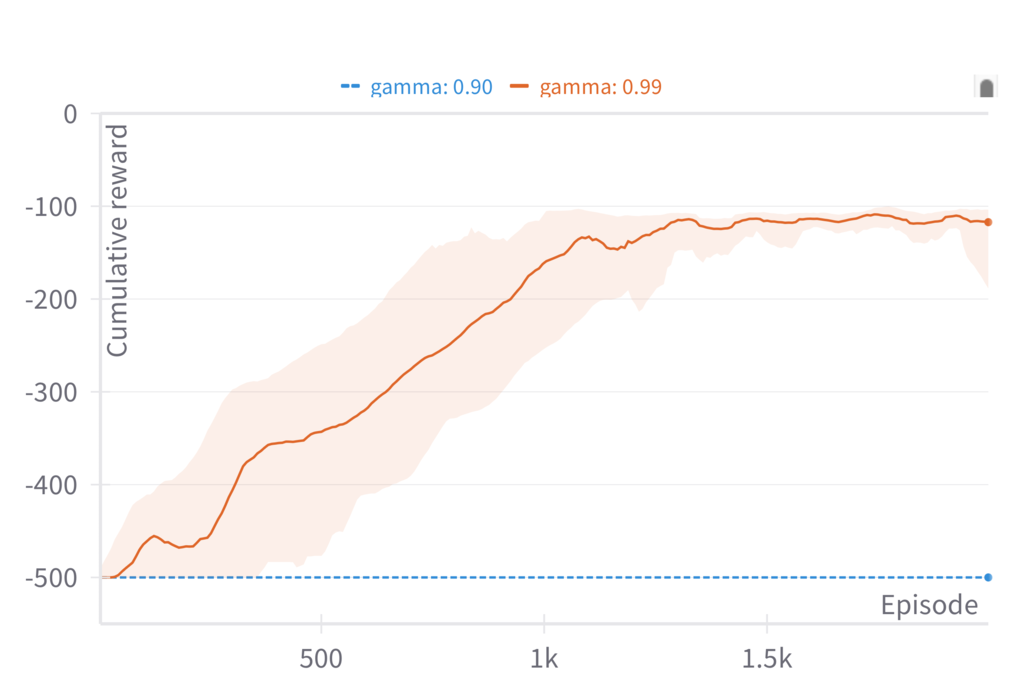
\includegraphics[width=\textwidth,height=3.125in]{figs/reward_default.png}
\end{center}

\marginnote{\begin{footnotesize}

``gamma'' = \(\gamma\) (discount factor)

\end{footnotesize}}

\subsection{\texorpdfstring{\(\ell^2\)
reward}{\textbackslash ell\^{}2 reward}}\label{ell2-reward}

\begin{center}
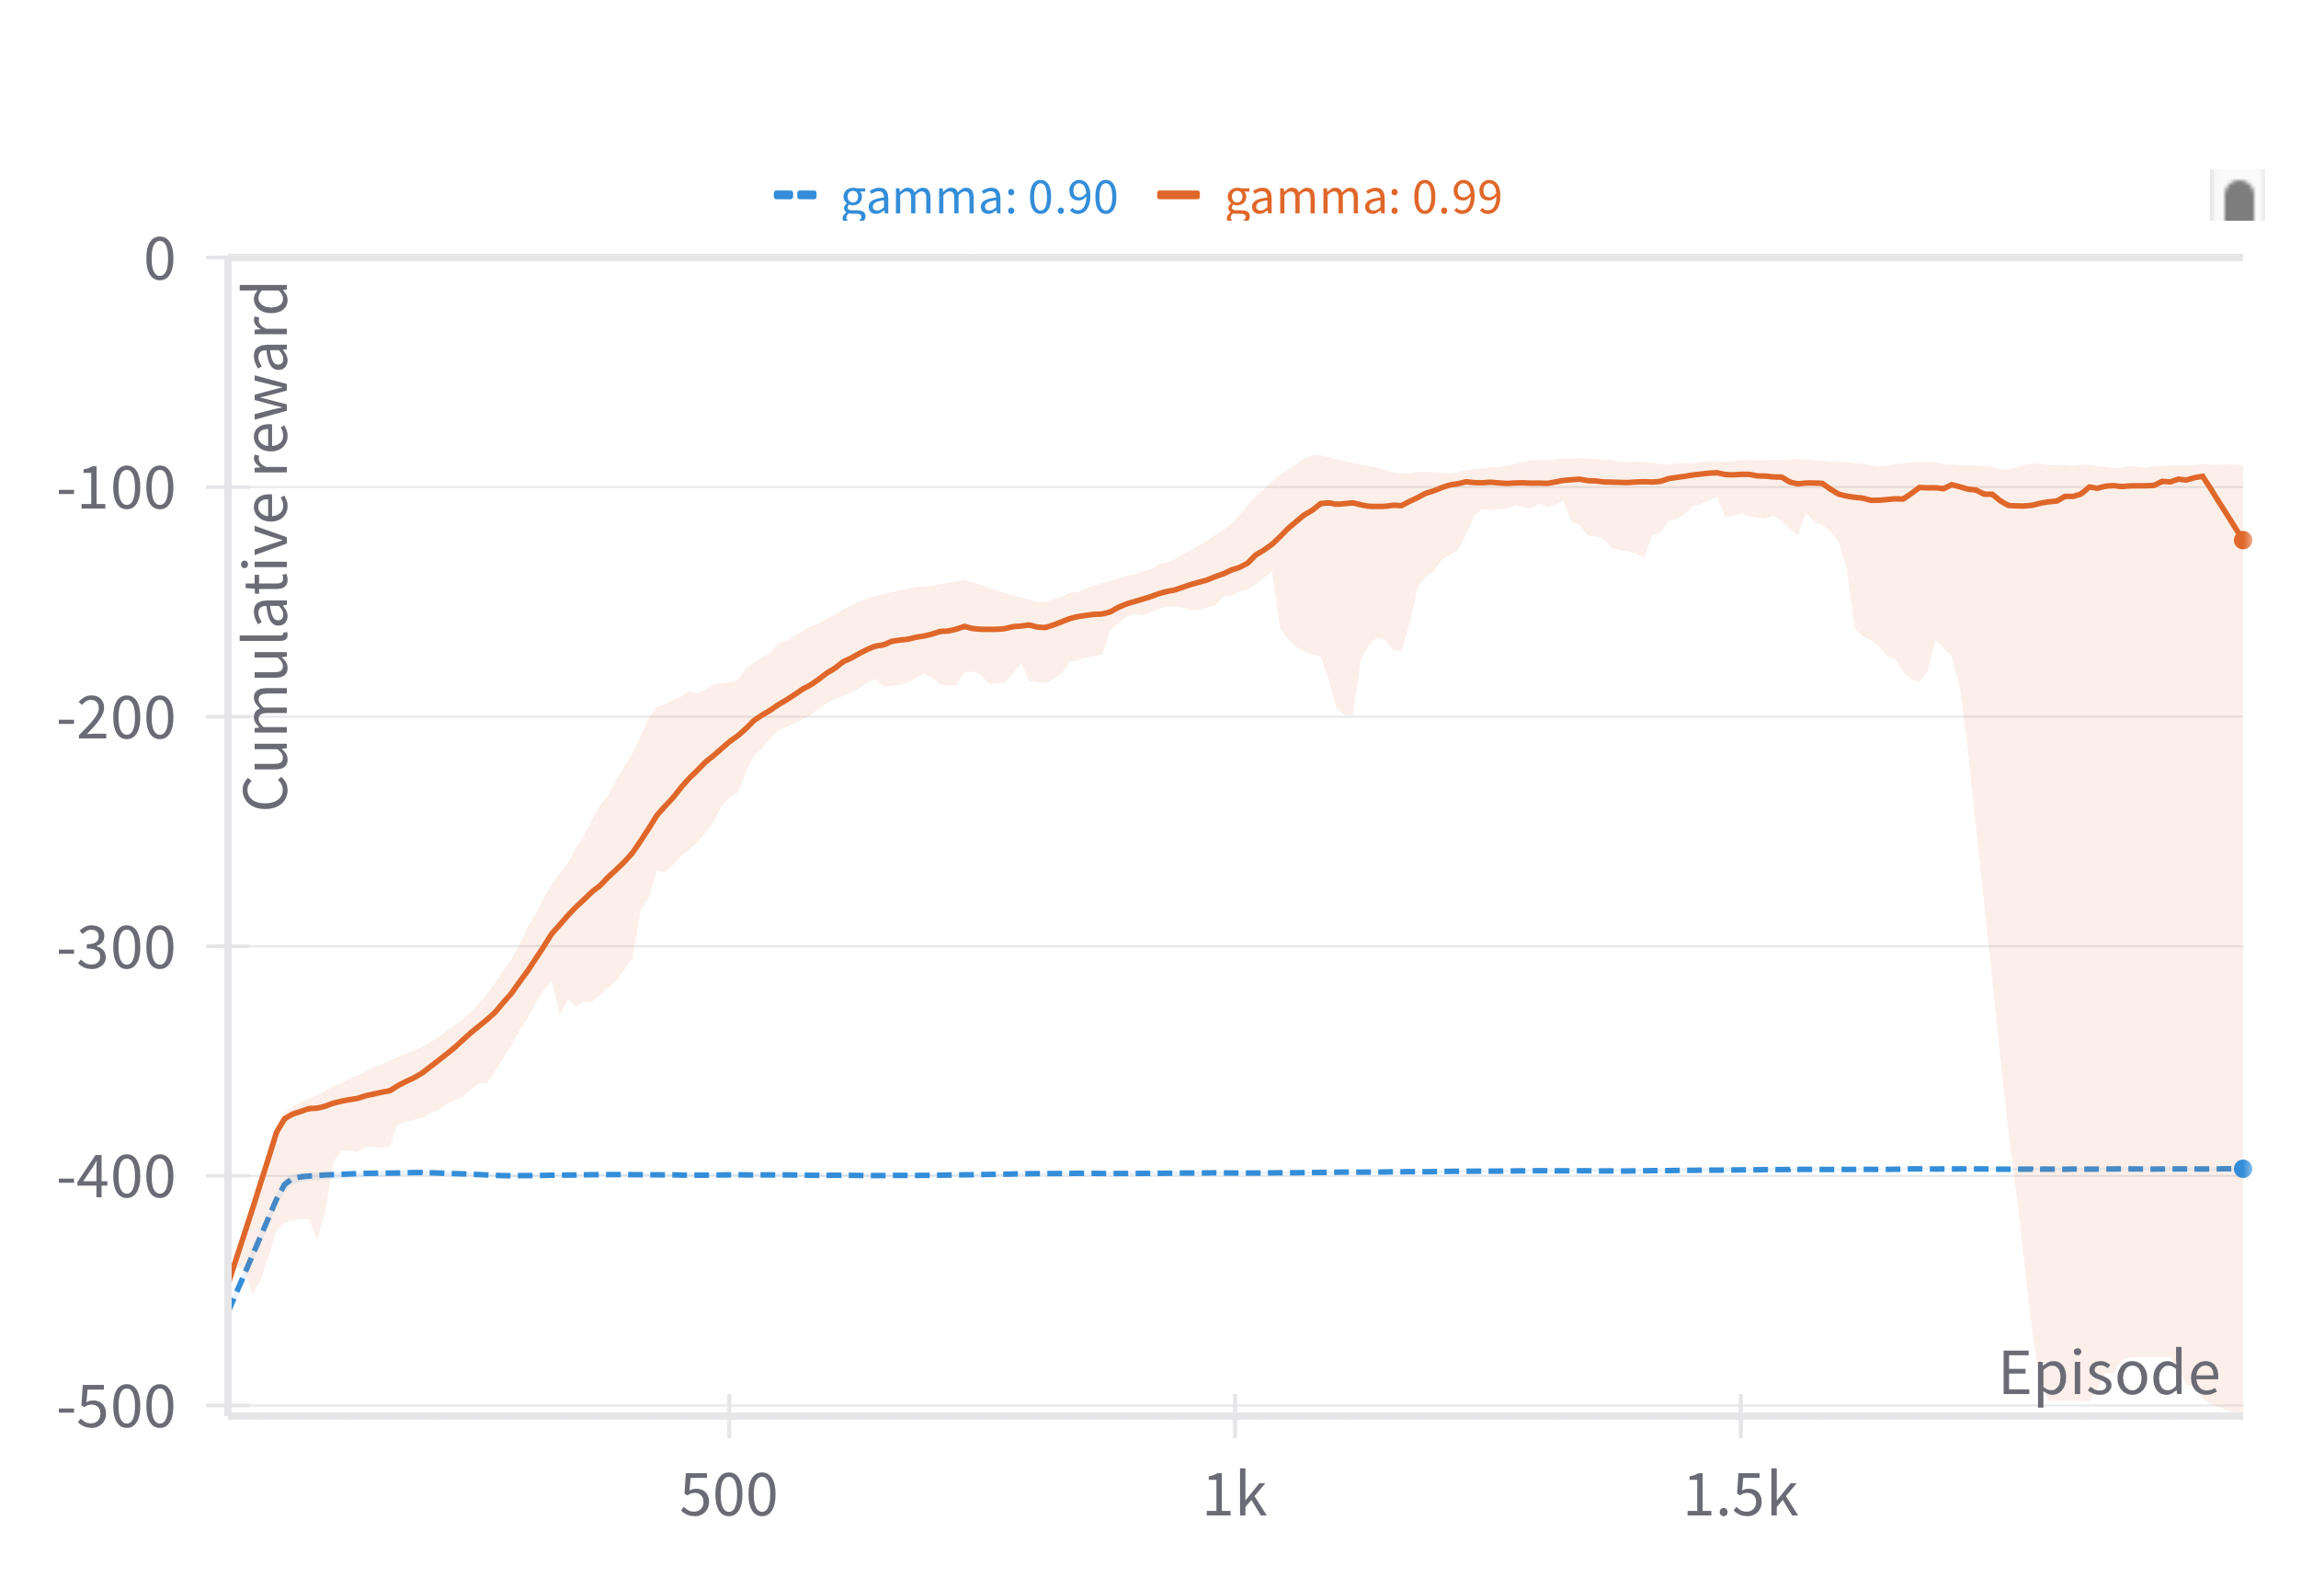
\includegraphics[width=\textwidth,height=3.125in]{figs/reward_l2.png}
\end{center}

\marginnote{\begin{footnotesize}

``gamma'' = \(\gamma\) (discount factor)

\end{footnotesize}}

\subsection{``Height'' reward}\label{height-reward}

\begin{center}
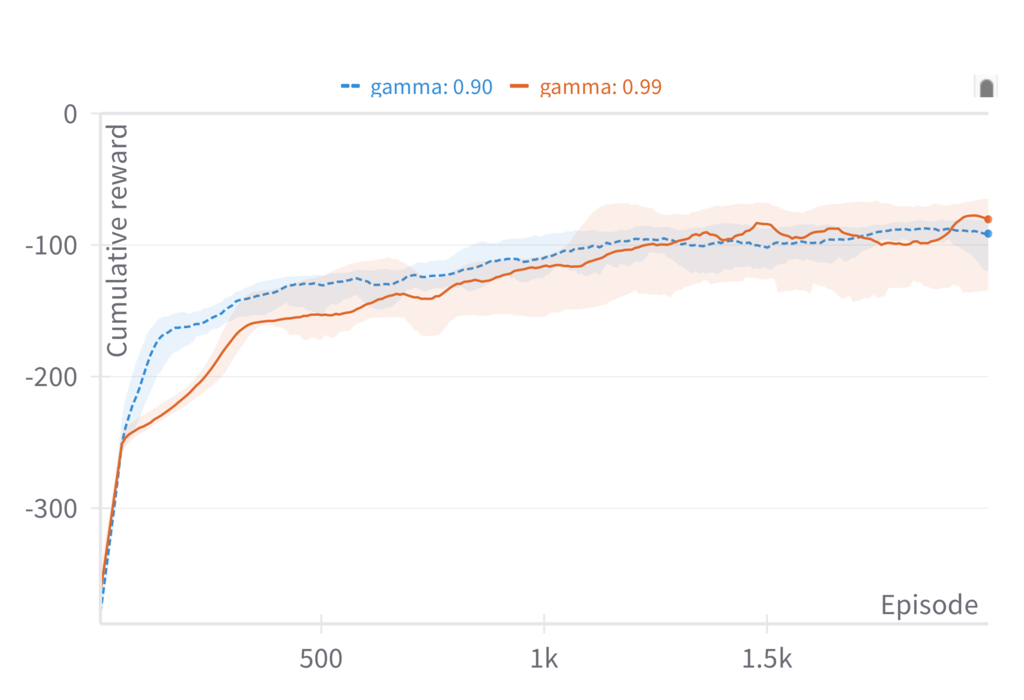
\includegraphics[width=\textwidth,height=3.125in]{figs/reward_height.png}
\end{center}

\marginnote{\begin{footnotesize}

``gamma'' = \(\gamma\) (discount factor)

\end{footnotesize}}

\subsection{\texorpdfstring{\(\ell^\infty\)
reward}{\textbackslash ell\^{}\textbackslash infty reward}}\label{ellinfty-reward}

\begin{center}
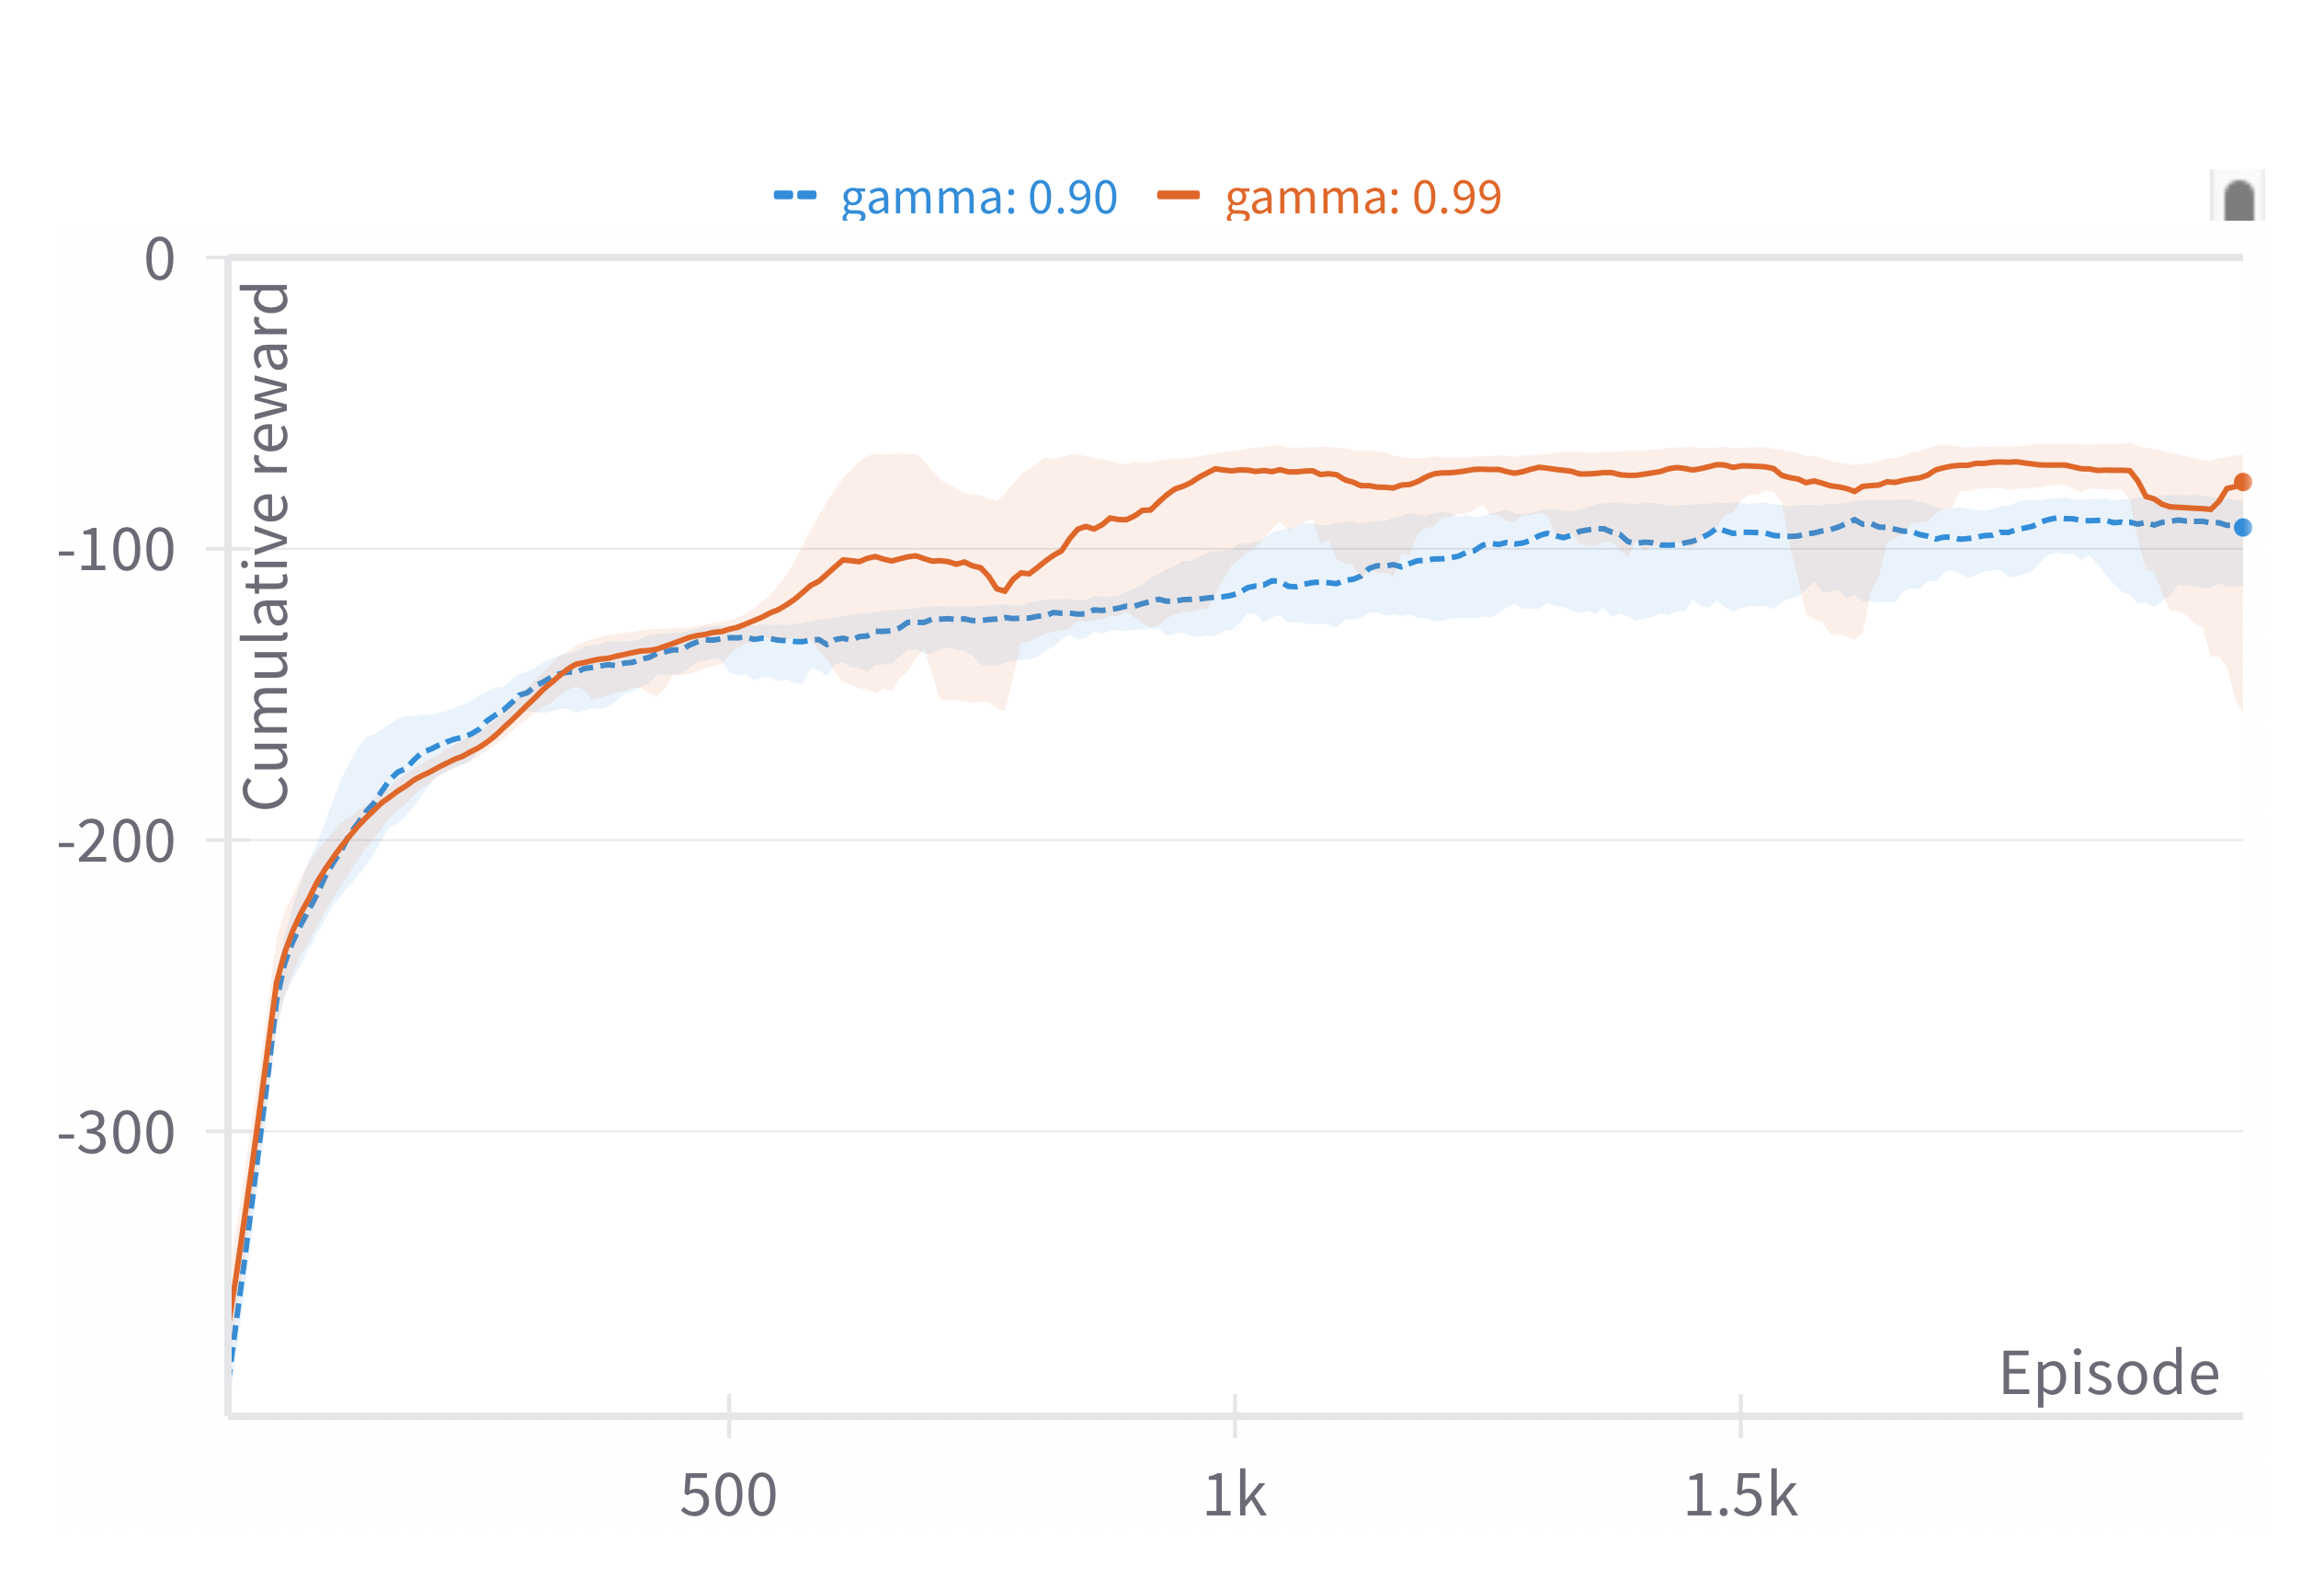
\includegraphics[width=\textwidth,height=3.125in]{figs/reward_linf.png}
\end{center}

\marginnote{\begin{footnotesize}

``gamma'' = \(\gamma\) (discount factor)

\end{footnotesize}}

\subsection{\texorpdfstring{Summary,
\(\gamma = 0.99\)}{Summary, \textbackslash gamma = 0.99}}\label{summary-gamma-0.99}

\begin{center}
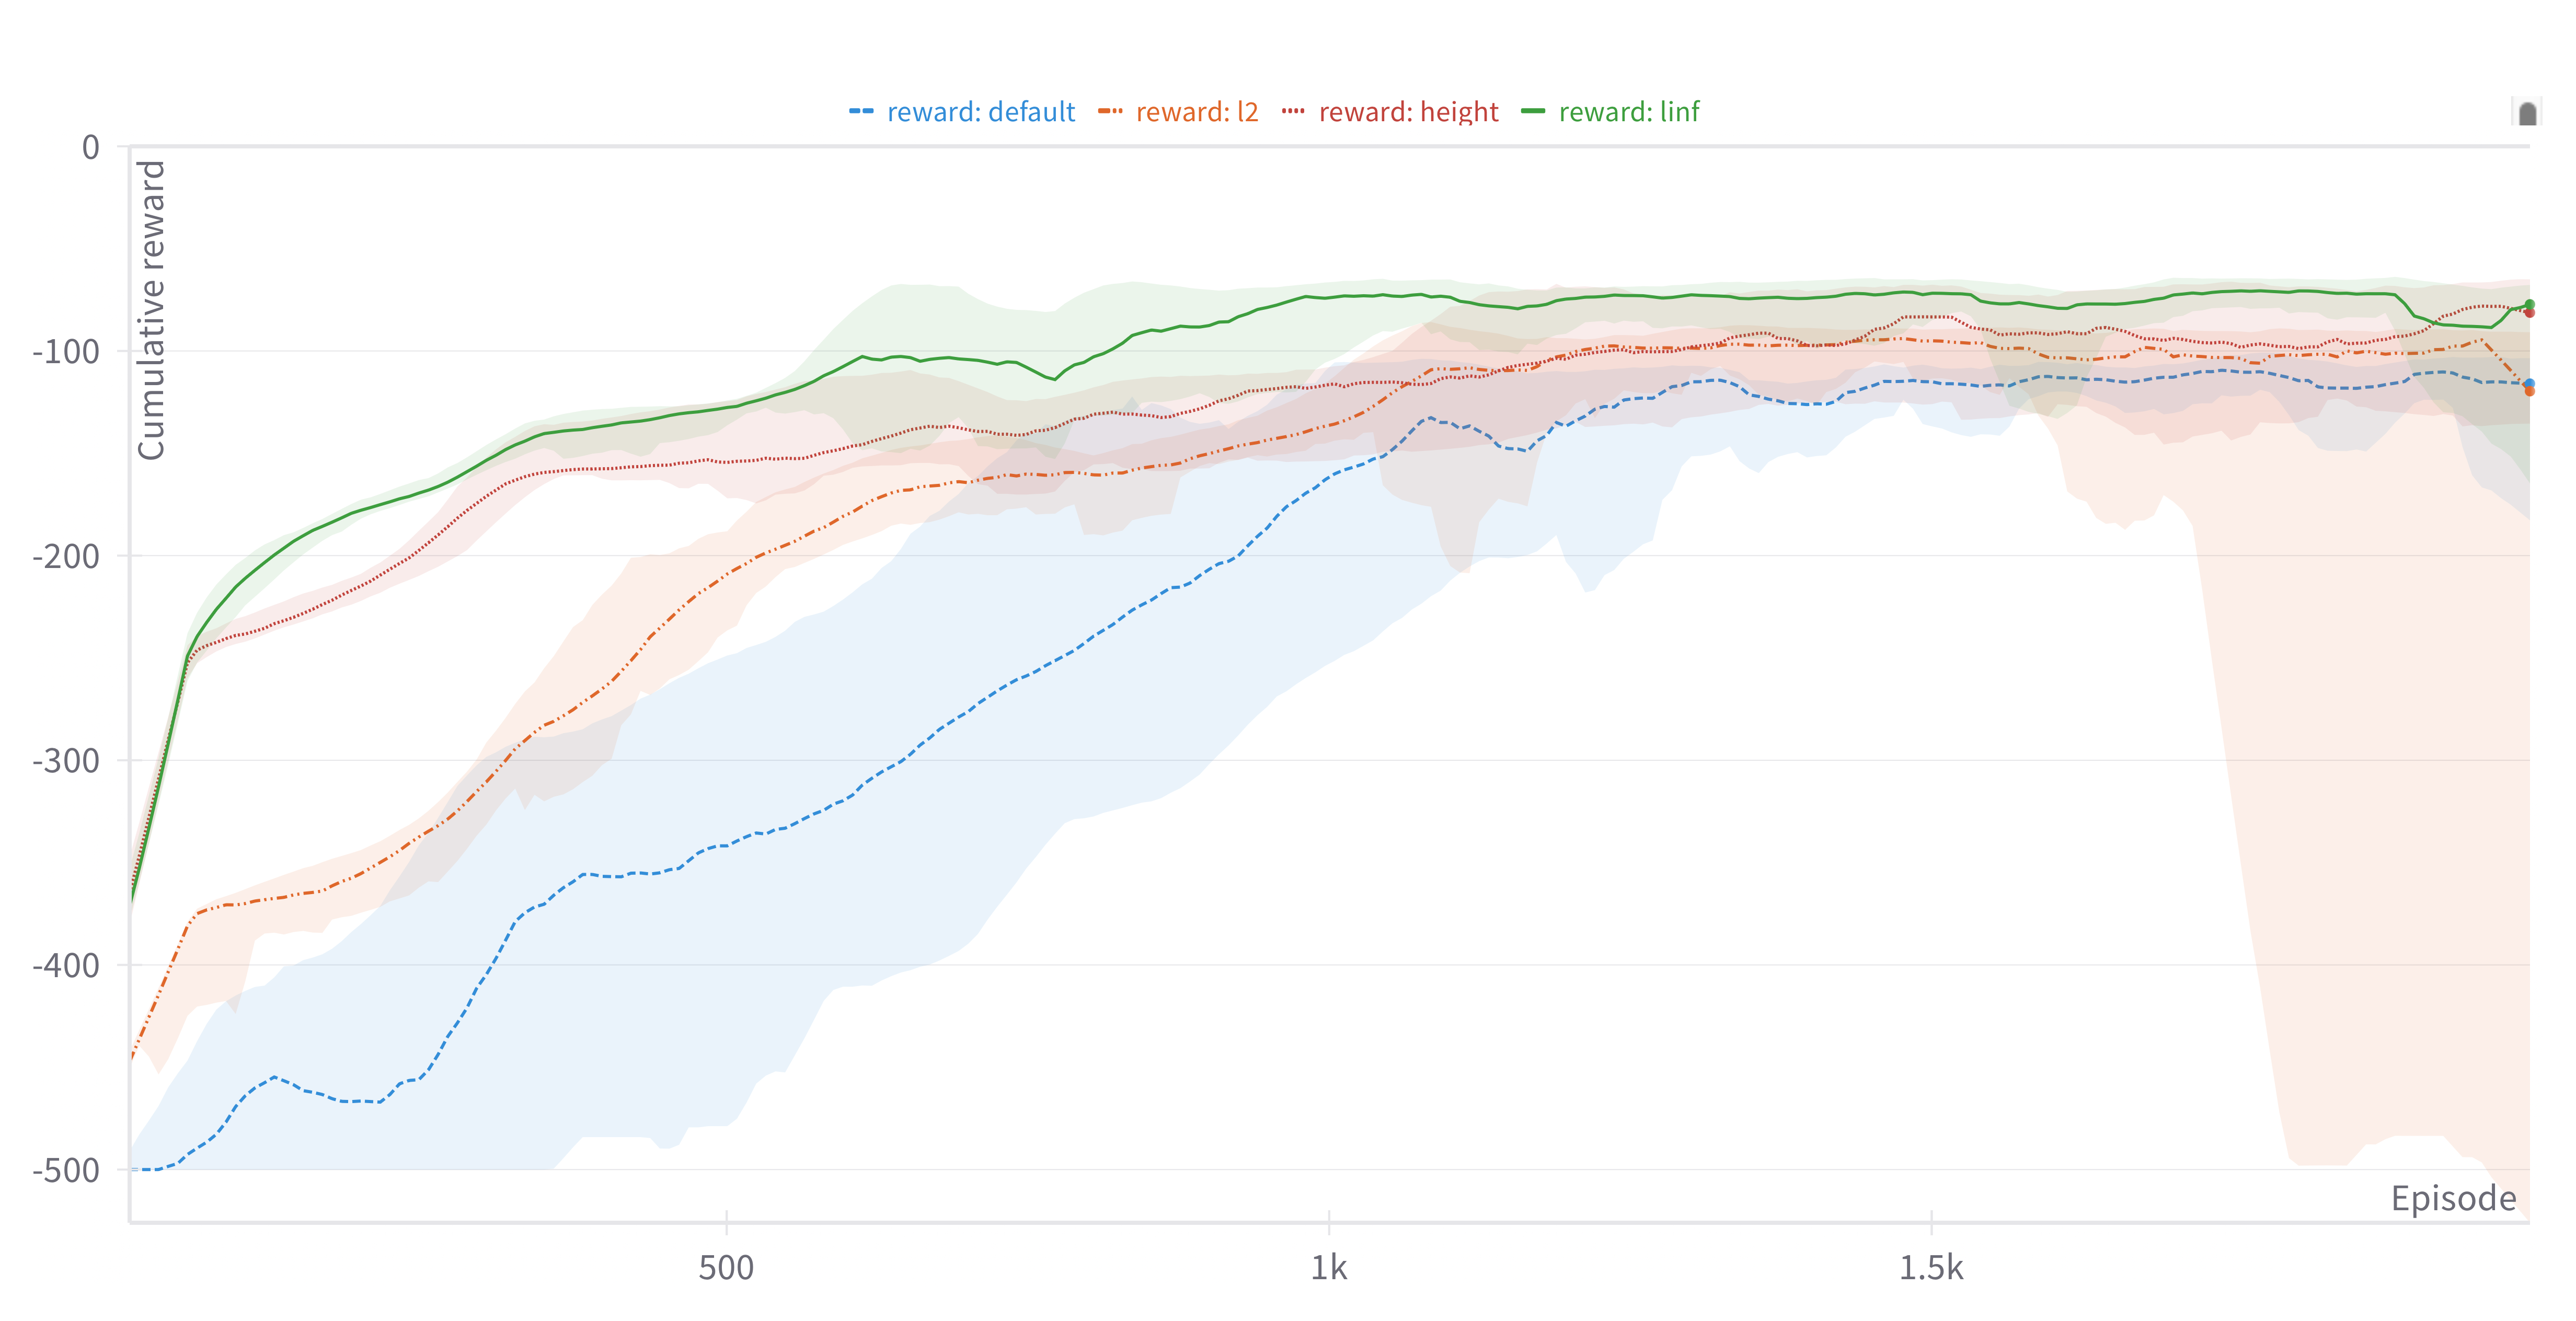
\includegraphics{figs/reward_gamma_99_all.png}
\end{center}

\begin{center}\rule{0.5\linewidth}{0.5pt}\end{center}

\begin{figure}

\begin{minipage}{0.20\linewidth}

\end{minipage}%
%
\begin{minipage}{0.20\linewidth}
default\end{minipage}%
%
\begin{minipage}{0.20\linewidth}
\(\ell^2\)\end{minipage}%
%
\begin{minipage}{0.20\linewidth}
height\end{minipage}%
%
\begin{minipage}{0.20\linewidth}
\(\ell^\infty\)\end{minipage}%
\newline
\begin{minipage}{0.20\linewidth}
\\
\strut \\
\(\gamma = 0.90\)\end{minipage}%
%
\begin{minipage}{0.20\linewidth}
\includegraphics{videos/gamma_90/acrobot-sac__default__1__episode-1950.mp4}\end{minipage}%
%
\begin{minipage}{0.20\linewidth}
\includegraphics{videos/gamma_90/acrobot-sac__l2__1__episode-1950.mp4}\end{minipage}%
%
\begin{minipage}{0.20\linewidth}
\includegraphics{videos/gamma_90/acrobot-sac__height__3__episode-1950.mp4}\end{minipage}%
%
\begin{minipage}{0.20\linewidth}
\includegraphics{videos/gamma_90/acrobot-sac__linf__1__episode-1950.mp4}\end{minipage}%
\newline
\begin{minipage}{0.20\linewidth}
\\
\strut \\
\(\gamma = 0.99\)\end{minipage}%
%
\begin{minipage}{0.20\linewidth}
\includegraphics{videos/gamma_99/acrobot-sac__default__0__episode-1950.mp4}\end{minipage}%
%
\begin{minipage}{0.20\linewidth}
\includegraphics{videos/gamma_99/acrobot-sac__l2__2__episode-1950.mp4}\end{minipage}%
%
\begin{minipage}{0.20\linewidth}
\includegraphics{videos/gamma_99/acrobot-sac__height__1__episode-1950.mp4}\end{minipage}%
%
\begin{minipage}{0.20\linewidth}
\includegraphics{videos/gamma_99/acrobot-sac__linf__2__episode-1950.mp4}\end{minipage}%

\end{figure}%

\marginnote{\begin{footnotesize}

1 of \(4^8\) configurations. Sampled via
\href{https://www.random.org}{random.org}.

\end{footnotesize}}

\subsection{Bloopers}\label{bloopers}

I modified the
\href{(https://github.com/Farama-Foundation/Gymnasium/blob/main/gymnasium/envs/classic_control/acrobot.py)}{default
environment}: default reward, spaces, sampling time

Action space:

\begin{itemize}
\tightlist
\item
  Old: \(\{-1, 0, 1\}\) (discrete)
\item
  Intermediate: \([-1, 1]\) (continuous, restricted)
\item
  New: \([-2, 2]\) (continuous, expanded)
\end{itemize}

Sampling time:

\begin{itemize}
\tightlist
\item
  Old: \(dt = 0.2\) seconds
\item
  New: \(dt = 0.1\) seconds
\end{itemize}

\subsection{Restricted action space}\label{restricted-action-space}

``Height'' reward, \(\gamma = 0.99\), 5hz

\includegraphics{videos/bloopers/5hz-smallTorque_gamma99_acrobat-sac__height__0__episode-1950.mp4}

\includegraphics[width=1\textwidth,height=\textheight]{figs/reward_blooper_height_gamma_99.png}

\subsection{Restricted action space
cont'd}\label{restricted-action-space-contd}

\(\ell^\infty\) reward, \(\gamma = 0.95\), 5hz

\includegraphics{videos/bloopers/5hz-smallTorque_gamma95_acrobat-sac__linf__0__episode-1950.mp4}

\includegraphics[width=1\textwidth,height=\textheight]{figs/reward_blooper_linf_gamma_95.png}

\subsection{An analytic solution: What if we know something about the
environment?}\label{an-analytic-solution-what-if-we-know-something-about-the-environment}

\subsection{The original problem}\label{the-original-problem}

\[\text{maximize }\quad \mathbb{E}_{\pi} \left[ \sum_{t=0}^{\infty} \gamma^t r(s_t,a_t)  \right]\]

\begin{itemize}
\tightlist
\item
  Unknown dynamics
\item
  Unstructured policy
\end{itemize}

\begin{itemize}
\tightlist
\item
  Possibly unknown reward
\item
  Everything is random
\end{itemize}

\subsection{Aside: Some notation}\label{aside-some-notation}

(placeholder -- some discussion about RL and control notation should go
somewhere\ldots)

\subsection{Let's grossly simplify the
problem}\label{lets-grossly-simplify-the-problem}

\begin{align}
\text{minimize } && \sum_{t=0}^{\infty} \gamma^t \left( x_t^2 + \rho u_t^2 \right)\\
\text{where } && x_{t+1} = a x_t + b u_t \\
&& u_t = -k x_t
\end{align}

\begin{itemize}
\tightlist
\item
  Linear, scalar dynamics
\item
  Linear policy
\end{itemize}

\begin{itemize}
\tightlist
\item
  Quadratic cost
\item
  Deterministic
\end{itemize}

\subsection{Assign some values for
simplicity}\label{assign-some-values-for-simplicity}

Focus on \(\gamma\) and \(k\):

\begin{align}
\text{minimize } && \sum_{t=0}^{\infty} \gamma^t \left( x_t^2 + u_t^2 \right)\\
\text{where } && x_{t+1} = 1.1 x_t + 0.5 u_t \\
&& u_t = -k x_t \\
&& x_0 = 1.0
\end{align}

\marginnote{\begin{footnotesize}

See \hyperref[gen_scalarLQR]{appendix} for general formulas

\end{footnotesize}}

\subsection{Trajectories are easy to
compute}\label{trajectories-are-easy-to-compute}

\begin{figure}

\begin{minipage}{0.46\linewidth}
\begin{align}
x_{t+1} &= 1.1 x_t + 0.5 u_t\\
u_t &= -k x_t
\end{align}\end{minipage}%
%
\begin{minipage}{0.09\linewidth}
\[\implies\]\end{minipage}%
%
\begin{minipage}{0.46\linewidth}
\begin{align}
x_{t+1} &= \left( 1.1 - 0.5 k \right)x_t \\
&\vdots\\
x_{t+1} &= \left( 1.1 - 0.5 k \right)^{t+1} \\
u_t &= -k \left( 1.1 - 0.5 k \right)^t
\end{align}\end{minipage}%

\end{figure}%

\subsection{Returns are easy to
compute}\label{returns-are-easy-to-compute}

\begin{align}
\sum_{t=0}^{\infty} \gamma^t \left( x_t^2 +  u_t^2 \right) &= 1 + \gamma (1.1-0.5k)^2 + \gamma^2 (1.1-0.5k)^4  + \ldots\\
&+  k^2  + \gamma  k^2 (1.1-0.5k)^2  + \ldots \\
&= \sum_{t=0}^{\infty} \gamma^t (1.1-0.5k)^{2t} (1 +  k^2) 
\end{align}

\marginnote{\begin{footnotesize}

\begin{align}
x_{t+1} &= \left( 1.1 - 0.5 k \right)^{t+1} x_0\\
u_t &= -k \left( 1.1 - 0.5 k \right)^t x_0 \\
x_0 &= 1.0
\end{align}

\end{footnotesize}}

\subsection{Quadratic value function}\label{quadratic-value-function}

By properties of geometric series:

\begin{align}
\text{return} &= \sum_{t=0}^{\infty} \gamma^t (1.1-0.5 k)^{2t} (1 +  k^2) \\
&= \frac{1 +  k^2}{1 - \gamma\left(1.1 - 0.5 k\right)^2} 
\end{align}

\marginnote{\begin{footnotesize}

\(\sum_{i = 0}^{\infty} \alpha \beta^i = \alpha \frac{1}{1 - \beta}\)

\end{footnotesize}}

\subsection{A 1-D optimization
problem}\label{a-1-d-optimization-problem}

\[\min_{k} \frac{1 +  k^2}{1 - \gamma\left(1.1 - 0.5 k\right)^2}\]

\subsection{A 1-D optimization
problem}\label{a-1-d-optimization-problem-1}

\[\min_{k} \frac{1 +  k^2}{1 - \gamma\left(1.1 - 0.5 k\right)^2}\]

\begin{figure}[H]

{\centering \includegraphics[width=\textwidth,height=3.64583in]{figs/desmos-controller.png}

}

\caption{Desmos
\href{https://www.desmos.com/calculator/vgnchtuqys}{{[}graph{]}}}

\end{figure}%

\begin{center}\rule{0.5\linewidth}{0.5pt}\end{center}

\begin{figure}

\begin{minipage}{0.33\linewidth}

\end{minipage}%
%
\begin{minipage}{0.33\linewidth}
\(\gamma = 1\)\end{minipage}%
%
\begin{minipage}{0.33\linewidth}
\(\gamma = 0\)\end{minipage}%
\newline
\begin{minipage}{0.33\linewidth}
Value function\end{minipage}%
%
\begin{minipage}{0.33\linewidth}
\includegraphics[width=\textwidth,height=1.82292in]{figs/desmos-controller.png}\end{minipage}%
%
\begin{minipage}{0.33\linewidth}
\includegraphics[width=\textwidth,height=1.82292in]{figs/desmos-gamma0-controller.png}\end{minipage}%
\newline
\begin{minipage}{0.33\linewidth}
Closed-loop trajectory\end{minipage}%
%
\begin{minipage}{0.33\linewidth}
\includegraphics[width=\textwidth,height=1.82292in]{figs/desmos-stable.png}\end{minipage}%
%
\begin{minipage}{0.33\linewidth}
\includegraphics[width=\textwidth,height=1.82292in]{figs/desmos-unstable.png}\end{minipage}%

\end{figure}%

\marginnote{\begin{footnotesize}

System: \(x_{t+1} = 1.1 x_t + 0.5 u_t\) (unstable)

\end{footnotesize}}

\subsection{Wait, are linear controllers
optimal?}\label{wait-are-linear-controllers-optimal}

YES!

\begin{align}
\min_{u_0, u_1, \ldots} && \sum_{t=0}^{\infty} \gamma^t \left( x_t^2 +  u_t^2 \right)\\
\text{where } && x_{t+1} = a x_t + b u_t \\
&& \require{enclose}\enclose{horizontalstrike}[mathcolor="red"]{\color{black}{u_t = -k x_t}}
\end{align}

\subsection{}\label{section-17}

Define
\[V^{\star}(x) = \min_{\begin{align} u_0, & u_1, \ldots \\ x_{t+1} &= a x_t + b u_t \\ x_0 &= x \end{align}} \sum_{t=0}^{\infty} \gamma^t \left( x_t^2 +  u_t^2 \right)\]

\[\Downarrow \text{(fact)}\]

\[V^{\star}(x) = P x^2\]

\subsection{}\label{section-18}

The optimal value function is:

\begin{enumerate}
\def\labelenumi{\arabic{enumi}.}
\tightlist
\item
  Quadratic
\item
  Parameterized by some \(P > 0\)
\end{enumerate}

\subsection{}\label{section-19}

Bellman gives us a single variable problem:
\[P x^2 = \min_{u} \left\{ x^2 +  u^2 + \gamma P\left( a x + b u \right)^2 \right\}\]

\[\Downarrow \text{solve } 0 = \nabla_u \left\{ \cdots \right\}\]

\[u = -\frac{\gamma a b P}{1 + \gamma b^2 P} x\]

\[\Downarrow\]

Linear controller\ldots but what is \(P\)?

\subsection{}\label{section-20}

Plug \(u\) back into the Bellman equation to find:
\[P = 1 + \gamma a^2 P - \frac{\gamma^2 (a b P)^2}{1 + \gamma b^2 P}\]

A fixed point in \(P\)!

Finding this fixed point in \textbf{parameter space} gives the optimal
solution in value \textbf{function space}

\subsection{}\label{section-21}

\subsection{Recap lessons from RL
section}\label{recap-lessons-from-rl-section}

(placeholder + 5 min break slide)

\section{Process control}\label{process-control}

\subsection{}\label{section-22}

A common control task is to bring a system to a constant value:

\begin{enumerate}
\def\labelenumi{\arabic{enumi}.}
\tightlist
\item
  Cruise control
\item
  Temperature
\item
  Concentrations
\end{enumerate}

\begin{enumerate}
\def\labelenumi{\arabic{enumi}.}
\setcounter{enumi}{3}
\tightlist
\item
  Levels
\item
  Moisture
\item
  Etc\ldots{}
\end{enumerate}

\begin{center}
\includegraphics[width=\textwidth,height=2.08333in]{figs/feedback_diagram.png}
\end{center}

\section{Linear policies}\label{linear-policies}

\section{PID control}\label{pid-control}

\emph{``Based on a survey of over eleven thousand controllers in the
refining, chemicals and pulp and paper industries, \textbf{97\% of
regulatory controllers utilize a PID} feedback control algorithm.''}

-- Desborough and Miller (2002), also Åström and Murray (2021)

\subsection{}\label{section-23}

\begin{figure}

\begin{minipage}{0.50\linewidth}
\includegraphics{figs/anim_impulse_u.gif}\end{minipage}%
%
\begin{minipage}{0.50\linewidth}
\includegraphics{figs/anim_impulse_y.gif}\end{minipage}%

\end{figure}%

The system settles at zero\ldots how do we get it to settle somewhere
else?

\subsection{Feedback control setup}\label{feedback-control-setup}

\(y_{sp}=\) desired value (sp = ``setpoint'')

\(y =\) measured value

\(e = y_{sp} - y\)

\textbf{We want \(e \to 0\) as \(t \to \infty\)}

\subsection{Proportional control}\label{proportional-control}

Consider the policy
\[u(t) = k_p e(t) \phantom{+ k_i \int_{0}^{t} e(\tau) d \tau}\]

\begin{figure}

\begin{minipage}{0.50\linewidth}
\includegraphics{figs/anim_P_u.gif}\end{minipage}%
%
\begin{minipage}{0.50\linewidth}
\includegraphics{figs/anim_P_y.gif}\end{minipage}%

\end{figure}%

\subsection{Proportional-Integral
control}\label{proportional-integral-control}

Consider the policy
\[u(t) = k_p e(t) + k_i \int_{0}^{t} e(\tau) d \tau\]

\begin{figure}

\begin{minipage}{0.50\linewidth}
\includegraphics{figs/anim_PI_u.gif}\end{minipage}%
%
\begin{minipage}{0.50\linewidth}
\includegraphics{figs/anim_PI_y.gif}\end{minipage}%

\end{figure}%

\subsection{The magic of integral
action}\label{the-magic-of-integral-action}

\begin{enumerate}
\def\labelenumi{\arabic{enumi}.}
\tightlist
\item
  Assume that \(k_p, k_i\) are chosen such that the system is stable
\item
  Then \(u(t) \to \bar{u}\), \(e(t) \to \bar{e}\)
\item
  We can write
  \[ \bar{u} = k_p \bar{e} + k_i \lim_{t \to \infty} \int_{0}^{t} e(\tau) d \tau\]
\item
  The integral term must converge
\item
  Zero offset!
\end{enumerate}

\subsection{Proportional-Integral-Derivative
control}\label{proportional-integral-derivative-control}

\includegraphics{figs/PID_Compensation_Animated.gif}

\textbf{Proportional:} Go towards the setpoint

\textbf{Integral:} Stay at the setpoint

\textbf{Derivative:} Don't overshoot the setpoint

\marginnote{\begin{footnotesize}

\href{https://en.wikipedia.org/w/index.php?title=Proportional–integral–derivative_controller&oldid=1221531928}{PID
controller (Wikipedia)}

\end{footnotesize}}

\subsection{PID summary}\label{pid-summary}

\textbf{Pros}

``Simple'' structure

Widely used

Stable, robust, offset-free tracking

\textbf{Cons}

``Simple'' systems

Can be difficult to tune

Awkward in the face of constraints

\marginnote{\begin{footnotesize}

See \hyperref[multiPID]{addendum} for details/experiments dealing with
multiloop PID

\end{footnotesize}}

\section{LQR}\label{lqr}

\subsection{Scalable design}\label{scalable-design}

\begin{align}
\min_{u_0, u_1, \ldots} && \sum_{t=0}^{\infty} \gamma^t \left( x_{t}^{T} M x_t +  u_{t}^{T} R u_t \right)\\
\text{where } && x_{t+1} = A x_t + B u_t \\
\end{align}

\begin{itemize}
\tightlist
\item
  \textbf{Linear:} Dynamics
\item
  \textbf{Quadratic:} Cost (and value)
\item
  \textbf{Regulator:} Keep state \(x_t\) around \(0\)
\end{itemize}

We already solved this in the scalar case!

\marginnote{\begin{footnotesize}

\(M \geq 0\), \(R >\), \(\gamma \in [0,1]\)

\end{footnotesize}}

\subsection{General solution}\label{general-solution}

\begin{enumerate}
\def\labelenumi{\arabic{enumi}.}
\tightlist
\item
  There is \(P > 0\) such that \(V^\star (x) = x^T P x\). Then via the
  \textbf{Bellman equation}
  \[x_{t}^{T} P x_t = \min_{u} \left\{ x_{t}^{T} M x_t +  u_{t}^{T} R u_t + \gamma \left( A x + B u \right)^{T} P \left( A x + B u \right) \right\}\]
\end{enumerate}

\subsection{General solution}\label{general-solution-1}

\begin{enumerate}
\def\labelenumi{\arabic{enumi}.}
\tightlist
\item
  Apply the \textbf{Bellman equation} with \(V^\star (x) = x^T P x\)
\end{enumerate}

\subsection{General solution}\label{general-solution-2}

\begin{enumerate}
\def\labelenumi{\arabic{enumi}.}
\tightlist
\item
  Apply the \textbf{Bellman equation} with \(V^\star (x) = x^T P x\)
\item
  Enforce \[0 = \nabla_u \left\{ \cdots \right\}\]
\end{enumerate}

\subsection{General solution}\label{general-solution-3}

\begin{enumerate}
\def\labelenumi{\arabic{enumi}.}
\tightlist
\item
  Apply the \textbf{Bellman equation} with \(V^\star (x) = x^T P x\)
\item
  Enforce \(0 = \nabla_u \left\{ \cdots \right\}\)
\item
  Obtain \(u = -K x\) where
  \[K = \gamma \left( R + \gamma B^T P B \right)^{-1} B^T P A\]
\end{enumerate}

\subsection{General solution}\label{general-solution-4}

\begin{enumerate}
\def\labelenumi{\arabic{enumi}.}
\tightlist
\item
  Apply the \textbf{Bellman equation} with \(V^\star (x) = x^T P x\)
\item
  Enforce \(0 = \nabla_u \left\{ \cdots \right\}\)
\item
  Obtain
  \(u = - \gamma \left( R + \gamma B^T P B \right)^{-1} B^T P A x\)
\item
  \(P\) satisfies the \textbf{Discrete Algebraic Riccati Equation}
  \[P = M + \gamma A^T P A - \gamma^2 A^T P B \left( R + \gamma B^T P B \right)^{-1} B^T P A\]
\end{enumerate}

\subsection{}\label{section-24}

\begin{itemize}
\item
  LQR is a tidy and globally optimal solution for controlling
  multivariable systems!
\item
  It comes standard in any control systems library
\end{itemize}

\begin{Shaded}
\begin{Highlighting}[numbers=left,,]
\ImportTok{using} \BuiltInTok{ControlSystems}

\NormalTok{Pd }\OperatorTok{=} \FunctionTok{c2d}\NormalTok{(}\FunctionTok{ss}\NormalTok{(P),ts)}
\NormalTok{A, B }\OperatorTok{=}\NormalTok{ Pd.A, Pd.B}
\NormalTok{M, R }\OperatorTok{=}\NormalTok{ I, I}

\NormalTok{K }\OperatorTok{=} \FunctionTok{lqr}\NormalTok{(Discrete, A, B, M, R)}

\FunctionTok{u}\NormalTok{(x,t)  }\OperatorTok{=} \OperatorTok{{-}}\NormalTok{K}\OperatorTok{*}\NormalTok{x}
\end{Highlighting}
\end{Shaded}

\marginnote{\begin{footnotesize}

Example is in the Julia package
\href{https://juliacontrol.github.io/ControlSystems.jl/dev/}{ControlSystems.jl}.
Other options include Matlab's
\href{https://www.mathworks.com/products/control.html}{Control System
Toolbox}, or
\href{https://python-control.readthedocs.io/en/latest/index.html}{Python
Control Systems Library}.

\end{footnotesize}}

\subsection{Aside about discounting}\label{aside-about-discounting}

Standard LQR solvers: \((A, B, M, R) \to K\)

Discounted LQR: Use
\[\left( \sqrt{\gamma} A, B, M, \frac{1}{\gamma} R \right)\]

As \(\gamma \to 0\)\ldots{}

\begin{itemize}
\tightlist
\item
  ``Ignore the state transition matrix''
\item
  ``Apply infinite weight to control actions''
\item
  \ldots Unstable controller
\end{itemize}

\subsection{}\label{section-25}

\includegraphics{figs/lqr_disturbance.png}

\begin{itemize}
\tightlist
\item
  The controller quickly brings the system to \(0\)
\item
  A random disturbance in \(u_2\) occurs at \(t = 15\), affecting
  \(y_1, y_2\)
\item
  The controller brings \(y_1\) and \(y_2\) back to equilibrium
\end{itemize}

\subsection{Globally optimal?}\label{globally-optimal}

All systems are subject to constraints:

\begin{itemize}
\tightlist
\item
  Finite resources \& money
\item
  Limited actuation
\end{itemize}

LQR assumes:

\begin{itemize}
\tightlist
\item
  Any control action is permissible
\item
  Any intermediate state is acceptable
\end{itemize}

\subsection{Globally optimal?}\label{globally-optimal-1}

Consider the system
\[x_{t+1} = \begin{bmatrix} 1 & 1\\ 0 & 1 \end{bmatrix} x_t + \begin{bmatrix} 1 \\ 0.5 \end{bmatrix} u_t\]

Unstable \(\to\) control is needed to achieve equilibrium

\subsection{Globally optimal?}\label{globally-optimal-2}

LQR, business as usual

\begin{center}
\includegraphics{figs/lqr_unconstrained.png}
\end{center}

\subsection{Globally optimal?}\label{globally-optimal-3}

Suppose only actions in the set
\(\left\{ u \colon \lVert u \rVert_{\infty} \leq 1 \right\}\) are
possible

And we want the states to stay in
\(\left\{ x \colon \lVert x \rVert_{\infty} \leq 5 \right\}\)

\begin{center}
\includegraphics{figs/lqr_constrained.png}
\end{center}

\subsection{Globally optimal?}\label{globally-optimal-4}

The actions can start out feasible, then become infeasible later

\begin{center}
\includegraphics{figs/lqr_constrained_later.png}
\end{center}

\subsection{Locally optimal}\label{locally-optimal}

\begin{center}
\includegraphics[width=\textwidth,height=4.16667in]{figs/lqr_constrainedSS.png}
\end{center}

\marginnote{\begin{footnotesize}

See Borrelli, Bemporad, and Morari (2017) or
\href{https://kwonlecture.snu.ac.kr/wp-content/uploads/2019/08/MPC_Course_v1.pdf}{slides}

\end{footnotesize}}

\subsection{Break}\label{break}

\begin{center}
\includegraphics{figs/Dunning-Kruger.jpg}
\end{center}

\section{Nonlinear policies}\label{nonlinear-policies}

\subsection{}\label{section-26}

What if a controller could anticipate an obstacle?

\subsection{}\label{section-27}

What if a controller could anticipate an obstacle?

\begin{center}
\includegraphics{figs/lane_change.png}
\end{center}

\subsection{}\label{section-28}

From this\ldots{}

\begin{center}
\includegraphics{figs/anim_dip_no-obstacle.gif}
\end{center}

\subsection{}\label{section-29}

To this\ldots{}

\begin{center}
\includegraphics{figs/anim_dip.gif}
\end{center}

\subsection{Anticipating constraints is inherently
nonlinear}\label{anticipating-constraints-is-inherently-nonlinear}

Suppose \(x_t\) is ``close'' to upper constraint \(c\):

\begin{itemize}
\tightlist
\item
  Take conservative actions near constraint
\item
  More freedom away from constraints
\end{itemize}

LQR:

\begin{itemize}
\tightlist
\item
  Follow \(u_t = -K x_t\) no matter what
\end{itemize}

\section{Model predictive control}\label{model-predictive-control}

\subsection{Problem formulation}\label{problem-formulation}

MPC is a common-sense strategy of making decisions by predicting the
future

\begin{align}
\min_{u_0, u_1, \ldots u_{N-1}} \quad & \sum_{t=0}^{N-1} x_{t}^{T} M x_t +  u_{t}^{T} R u_t \\
\text{where } \quad & x_{t+1} = A x_t + B u_t \\
& x_t \in \mathcal{X} \\
& u_t \in \mathcal{U}
\end{align}

\marginnote{\begin{footnotesize}

\(\mathcal{X}, \mathcal{U}\) are often box constraints:
\(u_{\min} \leq u_t \leq u_{\max} \forall t\). Like LQR,
\(M \geq 0, R > 0\).

\end{footnotesize}}

\subsection{Problem formulation}\label{problem-formulation-1}

Applying the optimal inputs \(u_0^\star, u_1^\star, \ldots\) is an
\textbf{open-loop} strategy

\begin{itemize}
\tightlist
\item
  Model errors compound
\item
  Unexpected disturbances will go unchecked
\item
  Will need to solve the MPC problem after \(N\) time steps anyway
\end{itemize}

\subsection{The receding horizon idea}\label{the-receding-horizon-idea}

At each time step, re-initialize the MPC problem with the state \(s_t\)
from the environment:

\begin{align}
\min_{u_0, u_1, \ldots u_{N-1}} \quad & \sum_{k=0}^{N-1} x_{k}^{T} M x_k +  u_{}^{T} R u_k \\
\text{where } \quad & \bbox[#FF9999,2pt]{x_0 = s_t} \\
& x_{k+1} = A x_k + B u_k \\
& x_k \in \mathcal{X} \\
& u_k \in \mathcal{U}
\end{align}

\subsection{The receding horizon
idea}\label{the-receding-horizon-idea-1}

MPC controller

\begin{enumerate}
\def\labelenumi{\arabic{enumi}.}
\tightlist
\item
  Initialize state \(x_0 = s\)
\item
  Solve the MPC optimization problem
\item
  Apply \(u_0^\star\) to the system
\item
  Update system state \(s \leftarrow s'\)
\end{enumerate}

\subsection{The receding horizon
idea}\label{the-receding-horizon-idea-2}

\begin{center}
\includegraphics[width=5.20833in,height=\textheight]{figs/receding_horizon.png}
\end{center}

\marginnote{\begin{footnotesize}

See Borrelli, Bemporad, and Morari (2017), Chapter 12

\end{footnotesize}}

\subsection{}\label{section-30}

\begin{figure}

\begin{minipage}{0.50\linewidth}
\includegraphics[width=\textwidth,height=3.64583in]{figs/mpc_closedlooptraj1.png}\end{minipage}%
%
\begin{minipage}{0.50\linewidth}
\includegraphics[width=\textwidth,height=4.16667in]{figs/mpc_closedlooptraj2.png}\end{minipage}%

\end{figure}%

Solid - realized closed-loop trajectories

Dash - predicted trajectory

\marginnote{\begin{footnotesize}

See Borrelli, Bemporad, and Morari (2017), Chapter 12

\end{footnotesize}}

\subsection{}\label{section-31}

\begin{figure}

\begin{minipage}{0.50\linewidth}
LQR\end{minipage}%
%
\begin{minipage}{0.50\linewidth}
MPC\end{minipage}%
\newline
\begin{minipage}{0.50\linewidth}
\includegraphics[width=\textwidth,height=4.16667in]{figs/lqr_constrainedSS.png}\end{minipage}%
%
\begin{minipage}{0.50\linewidth}
\includegraphics[width=\textwidth,height=4.16667in]{figs/mpc_constrainedSS.png}\end{minipage}%

\end{figure}%

\marginnote{\begin{footnotesize}

Check \hyperref[mpcisnonlinear]{addendum} to see why MPC is a nonlinear
controller

\end{footnotesize}}

\subsection{Stability issues}\label{stability-issues}

\emph{``In the engineering literature it is often assumed (tacitly and
incorrectly) that a system with optimal control law is necessarily
stable.''}

-- Kalman (1960)

\subsection{}\label{section-32}

Repeatedly implementing a finite horizon solution on an infinite horizon
problem leads to ``surprises''

\begin{itemize}
\tightlist
\item
  Infeasibility
\item
  Instability
\end{itemize}

\subsection{}\label{section-33}

How can we solve an infinite horizon optimal control problem with finite
resources?

\begin{enumerate}
\def\labelenumi{\arabic{enumi}.}
\tightlist
\item
  Terminal constraint
\item
  Terminal cost
\end{enumerate}

\begin{align}
\min_{u_0, u_1, \ldots u_{N-1}} \quad & \sum_{k=0}^{N-1} \left( x_{k}^{T} M x_k +  u_{k}^{T} R u_k \right) + \bbox[#FF9999,2pt]{x_{N}^{T} P x_{N}}\\
\text{where } \quad & x_0 = s_t \\
& x_{k+1} = A x_k + B u_k \\
& x_k \in \mathcal{X}, u_k \in \mathcal{U} \\
& \bbox[#FF9999,2pt]{x_{N} \in \mathcal{X}_f}
\end{align}

\subsection{}\label{section-34}

How to design terminal cost?

LQR!

\begin{enumerate}
\def\labelenumi{\arabic{enumi}.}
\tightlist
\item
  Obtain \(P\) by solving \(\texttt{lqr}(A, B, M, R)\)
\item
  Embed a fictitious LQR controller \(u_t = -K x_t\) into MPC after
  \(N_c\) time steps
\end{enumerate}

\subsection{Final objective}\label{final-objective}

\begin{align}
\min_{u_0, u_1, \ldots u_{N_c - 1}} \quad & \sum_{k=0}^{N-1} \left( x_{k}^{T} M x_k +  u_{k}^{T} R u_k \right) + x_{N}^{T} P x_{N}\\
\text{where }\quad & x_0 = s_t \\
& x_{k+1} = A x_k + B u_k \\
& x_k \in \mathcal{X},\quad u_k \in \mathcal{U} \\
& u_{k} = -K x_k,\quad N_c \leq k < N
\end{align}

Mimic infinite horizon behavior

\subsection{}\label{section-35}

\begin{center}
\includegraphics{figs/cl.gif}
\end{center}

\section{MPC + RL}\label{mpc-rl}

\begin{center}
\includegraphics{figs/rl_mpc_tree.png}
\end{center}

\marginnote{\begin{footnotesize}

Arroyo et al. (2022)

\end{footnotesize}}

\subsection{Main motivation}\label{main-motivation}

MPC

Safety by design

Modularity

Manual design

Rigid

RL

Model-free

Flexible objectives

Safety constraints

Slowish learning

\subsection{MPC + value function}\label{mpc-value-function}

\begin{align}
\min_{u_0, u_1, \ldots u_{N - 1}} \quad & \sum_{k=0}^{N-1} \ell(x_k, u_k) \phantom{\quad + \overbrace{V_{\theta}(x_N)}^{\text{Learnable residual}}}\\
\text{where }\quad & x_0 = s_t \\
& x_{k+1} = f(x_k, u_k) \\
& \underbrace{x_k \in \mathcal{X},\quad u_k \in \mathcal{U}}_{\text{Prior engineering}} \\
\end{align}

\begin{align}
\min_{u_0, u_1, \ldots u_{N - 1}} \quad & \sum_{k=0}^{N-1} \ell(x_k, u_k)\quad + \overbrace{V_{\theta}(x_N)}^{\text{Learnable residual}}\\
\text{where }\quad & x_0 = s_t \\
& x_{k+1} = f(x_k, u_k) \\
& \underbrace{x_k \in \mathcal{X},\quad u_k \in \mathcal{U}}_{\text{Prior engineering}} \\
\end{align}

\begin{align}
\min_{u_0, u_1, \ldots u_{N - 1}} & \sum_{k=0}^{N-1} \ell(x_k, u_k) + V_{\theta}(x_N)\\
\text{where }\quad & x_0 = s_t \\
& x_{k+1} = f(x_k, u_k) \\
& x_k \in \mathcal{X},\quad u_k \in \mathcal{U} \\
\end{align}

\subsection{Break}\label{break-1}

\begin{center}
\includegraphics{figs/Chaotic+Grad+Student+HiRes.jpg}
\end{center}

\section{Implementation}\label{implementation}

\subsection{MPC frameworks}\label{mpc-frameworks}

\begin{figure}

\begin{minipage}{0.33\linewidth}

\begin{figure}[H]

{\centering \includegraphics[width=\textwidth,height=1.04167in]{figs/package_optimization-engine.png}

}

\subcaption{Sopasakis, Fresk, and Patrinos (2020)}

\end{figure}%

\end{minipage}%
%
\begin{minipage}{0.33\linewidth}

\begin{figure}[H]

{\centering \includegraphics[width=\textwidth,height=1.5625in]{figs/package_dompc.png}

}

\subcaption{Fiedler et al. (2023)}

\end{figure}%

\end{minipage}%
%
\begin{minipage}{0.33\linewidth}

\begin{figure}[H]

{\centering \includegraphics[width=\textwidth,height=1.04167in]{figs/package_mathworks.png}

}

\subcaption{\href{https://www.mathworks.com/products/model-predictive-control.html}{Model
Predictive Control Toolbox}}

\end{figure}%

\end{minipage}%
\newline
\begin{minipage}{0.50\linewidth}

\begin{figure}[H]

{\centering \includegraphics[width=\textwidth,height=0.52083in]{figs/package_acados.png}

}

\subcaption{Verschueren et al. (2022)}

\end{figure}%

\end{minipage}%
%
\begin{minipage}{0.50\linewidth}

\begin{figure}[H]

{\centering \includegraphics[width=\textwidth,height=0.52083in]{figs/package_grampc.png}

}

\subcaption{Englert et al. (2019)}

\end{figure}%

\end{minipage}%
\newline
\begin{minipage}{0.50\linewidth}

\begin{figure}[H]

{\centering \includegraphics[width=\textwidth,height=0.52083in]{figs/package_matmpc.png}

}

\subcaption{Chen et al. (2019)}

\end{figure}%

\end{minipage}%
%
\begin{minipage}{0.50\linewidth}

\begin{figure}[H]

{\centering \includegraphics[width=\textwidth,height=0.52083in]{figs/package_mpctools.png}

}

\subcaption{\href{https://sites.engineering.ucsb.edu/~jbraw/software/mpctools/examples/index.html}{MPC
Tools}}

\end{figure}%

\end{minipage}%

\end{figure}%

\subsection{MPC frameworks}\label{mpc-frameworks-1}

\href{https://www.do-mpc.com/en/latest/}{do-mpc}:

\begin{itemize}
\tightlist
\item
  Open source
\item
  Modular
\end{itemize}

\begin{itemize}
\tightlist
\item
  Python interface
\item
  Fast
\end{itemize}

\begin{figure}

\begin{minipage}{0.50\linewidth}

\begin{figure}[H]

{\centering \includegraphics[width=\textwidth,height=1.5625in]{figs/package_dompc.png}

}

\subcaption{Fiedler et al. (2023)}

\end{figure}%

\end{minipage}%
%
\begin{minipage}{0.50\linewidth}

\begin{figure}[H]

{\centering \includegraphics[width=\textwidth,height=1.5625in]{figs/casadi_logo.png}

}

\subcaption{Andersson et al. (2019)}

\end{figure}%

\end{minipage}%

\end{figure}%

\subsection{Example: Triple mass spring
system}\label{example-triple-mass-spring-system}

\begin{figure}

\begin{minipage}{0.46\linewidth}
\includegraphics{figs/anim_disc_3d_uncontrolled.gif}\end{minipage}%
%
\begin{minipage}{0.09\linewidth}
\[\rightarrow\]\end{minipage}%
%
\begin{minipage}{0.46\linewidth}
\includegraphics{figs/anim_disc_3d_ctrl_motor.gif}\end{minipage}%

\end{figure}%

\marginnote{\begin{footnotesize}

See
\href{https://github.com/do-mpc/do-mpc/blob/master/documentation/source/getting_started.ipynb}{notebook}
from \href{https://www.do-mpc.com/en/latest/index.html}{do-mpc} for full
code samples. We only show snippets of the key destinations.

\end{footnotesize}}

\subsection{Create model}\label{create-model}

\begin{Shaded}
\begin{Highlighting}[numbers=left,,]
\ImportTok{import}\NormalTok{ do\_mpc}
\ImportTok{from}\NormalTok{ casadi }\ImportTok{import} \OperatorTok{*}

\NormalTok{model\_type }\OperatorTok{=} \StringTok{\textquotesingle{}continuous\textquotesingle{}} \CommentTok{\# either \textquotesingle{}discrete\textquotesingle{} or \textquotesingle{}continuous\textquotesingle{}}
\NormalTok{model }\OperatorTok{=}\NormalTok{ do\_mpc.model.Model(model\_type)}

\NormalTok{dphi }\OperatorTok{=}\NormalTok{ model.set\_variable(var\_type}\OperatorTok{=}\StringTok{\textquotesingle{}\_x\textquotesingle{}}\NormalTok{, var\_name}\OperatorTok{=}\StringTok{\textquotesingle{}dphi\textquotesingle{}}\NormalTok{, shape}\OperatorTok{=}\NormalTok{(}\DecValTok{3}\NormalTok{,}\DecValTok{1}\NormalTok{))}
\CommentTok{\# Two states for the desired (set) motor position:}
\NormalTok{phi\_m\_1\_set }\OperatorTok{=}\NormalTok{ model.set\_variable(var\_type}\OperatorTok{=}\StringTok{\textquotesingle{}\_u\textquotesingle{}}\NormalTok{, var\_name}\OperatorTok{=}\StringTok{\textquotesingle{}phi\_m\_1\_set\textquotesingle{}}\NormalTok{)}
\NormalTok{phi\_m\_2\_set }\OperatorTok{=}\NormalTok{ model.set\_variable(var\_type}\OperatorTok{=}\StringTok{\textquotesingle{}\_u\textquotesingle{}}\NormalTok{, var\_name}\OperatorTok{=}\StringTok{\textquotesingle{}phi\_m\_2\_set\textquotesingle{}}\NormalTok{)}
\end{Highlighting}
\end{Shaded}

\begin{center}
\includegraphics[width=\textwidth,height=2.08333in]{figs/triple_mass_spring.png}
\end{center}

\subsection{Right-hand-side equation}\label{right-hand-side-equation}

Define the states, inputs, parameters, and function composing an ODE
\[\dot{x} = f(x, u)\]

\begin{Shaded}
\begin{Highlighting}[numbers=left,,]
\NormalTok{Theta\_1 }\OperatorTok{=}\NormalTok{ model.set\_variable(}\StringTok{\textquotesingle{}parameter\textquotesingle{}}\NormalTok{, }\StringTok{\textquotesingle{}Theta\_1\textquotesingle{}}\NormalTok{) }
\NormalTok{Theta\_2 }\OperatorTok{=}\NormalTok{ model.set\_variable(}\StringTok{\textquotesingle{}parameter\textquotesingle{}}\NormalTok{, }\StringTok{\textquotesingle{}Theta\_2\textquotesingle{}}\NormalTok{)}
\NormalTok{Theta\_3 }\OperatorTok{=}\NormalTok{ model.set\_variable(}\StringTok{\textquotesingle{}parameter\textquotesingle{}}\NormalTok{, }\StringTok{\textquotesingle{}Theta\_3\textquotesingle{}}\NormalTok{)}

\NormalTok{c }\OperatorTok{=}\NormalTok{ np.array([}\FloatTok{2.697}\NormalTok{,  }\FloatTok{2.66}\NormalTok{,  }\FloatTok{3.05}\NormalTok{, }\FloatTok{2.86}\NormalTok{])}\OperatorTok{*}\FloatTok{1e{-}3}
\NormalTok{d }\OperatorTok{=}\NormalTok{ np.array([}\FloatTok{6.78}\NormalTok{,  }\FloatTok{8.01}\NormalTok{,  }\FloatTok{8.82}\NormalTok{])}\OperatorTok{*}\FloatTok{1e{-}5}

\NormalTok{dphi\_next }\OperatorTok{=}\NormalTok{ vertcat(}
    \OperatorTok{{-}}\NormalTok{c[}\DecValTok{0}\NormalTok{]}\OperatorTok{/}\NormalTok{Theta\_1}\OperatorTok{*}\NormalTok{(phi\_1}\OperatorTok{{-}}\NormalTok{phi\_1\_m)}\OperatorTok{{-}}\NormalTok{c[}\DecValTok{1}\NormalTok{]}\OperatorTok{/}\NormalTok{Theta\_1}\OperatorTok{*}\NormalTok{(phi\_1}\OperatorTok{{-}}\NormalTok{phi\_2)}\OperatorTok{{-}}\NormalTok{d[}\DecValTok{0}\NormalTok{]}\OperatorTok{/}\NormalTok{Theta\_1}\OperatorTok{*}\NormalTok{dphi[}\DecValTok{0}\NormalTok{],}
    \OperatorTok{{-}}\NormalTok{c[}\DecValTok{1}\NormalTok{]}\OperatorTok{/}\NormalTok{Theta\_2}\OperatorTok{*}\NormalTok{(phi\_2}\OperatorTok{{-}}\NormalTok{phi\_1)}\OperatorTok{{-}}\NormalTok{c[}\DecValTok{2}\NormalTok{]}\OperatorTok{/}\NormalTok{Theta\_2}\OperatorTok{*}\NormalTok{(phi\_2}\OperatorTok{{-}}\NormalTok{phi\_3)}\OperatorTok{{-}}\NormalTok{d[}\DecValTok{1}\NormalTok{]}\OperatorTok{/}\NormalTok{Theta\_2}\OperatorTok{*}\NormalTok{dphi[}\DecValTok{1}\NormalTok{],}
    \OperatorTok{{-}}\NormalTok{c[}\DecValTok{2}\NormalTok{]}\OperatorTok{/}\NormalTok{Theta\_3}\OperatorTok{*}\NormalTok{(phi\_3}\OperatorTok{{-}}\NormalTok{phi\_2)}\OperatorTok{{-}}\NormalTok{c[}\DecValTok{3}\NormalTok{]}\OperatorTok{/}\NormalTok{Theta\_3}\OperatorTok{*}\NormalTok{(phi\_3}\OperatorTok{{-}}\NormalTok{phi\_2\_m)}\OperatorTok{{-}}\NormalTok{d[}\DecValTok{2}\NormalTok{]}\OperatorTok{/}\NormalTok{Theta\_3}\OperatorTok{*}\NormalTok{dphi[}\DecValTok{2}\NormalTok{],}
\NormalTok{)}

\NormalTok{model.set\_rhs(}\StringTok{\textquotesingle{}dphi\textquotesingle{}}\NormalTok{, dphi\_next)}
\NormalTok{model.setup()}
\end{Highlighting}
\end{Shaded}

\subsection{Create controller}\label{create-controller}

\begin{Shaded}
\begin{Highlighting}[numbers=left,,]
\NormalTok{mpc }\OperatorTok{=}\NormalTok{ do\_mpc.controller.MPC(model)}

\NormalTok{setup\_mpc }\OperatorTok{=}\NormalTok{ \{}
    \StringTok{\textquotesingle{}n\_horizon\textquotesingle{}}\NormalTok{: }\DecValTok{20}\NormalTok{,}
    \StringTok{\textquotesingle{}t\_step\textquotesingle{}}\NormalTok{: }\FloatTok{0.1}\NormalTok{,}
    \StringTok{\textquotesingle{}n\_robust\textquotesingle{}}\NormalTok{: }\DecValTok{1}\NormalTok{,}
    \StringTok{\textquotesingle{}store\_full\_solution\textquotesingle{}}\NormalTok{: }\VariableTok{True}\NormalTok{,}
\NormalTok{\}}
\NormalTok{mpc.set\_param(}\OperatorTok{**}\NormalTok{setup\_mpc)}
\end{Highlighting}
\end{Shaded}

(Defining constraints, the objective function, and even uncertain
parameters, all follow a similar workflow )

\begin{Shaded}
\begin{Highlighting}[]
\NormalTok{mpc.setup()}
\end{Highlighting}
\end{Shaded}

\subsection{Define simulator}\label{define-simulator}

Either use the same model inside the MPC or define a different model to
simulate the ``true'' system:

\begin{itemize}
\tightlist
\item
  Simplified MPC model
\item
  Complex ``true'' simulator model
\end{itemize}

\begin{Shaded}
\begin{Highlighting}[]
\NormalTok{simulator }\OperatorTok{=}\NormalTok{ do\_mpc.simulator.Simulator(model)}
\end{Highlighting}
\end{Shaded}

\subsection{Run the control loop}\label{run-the-control-loop}

\begin{Shaded}
\begin{Highlighting}[]
\ControlFlowTok{for}\NormalTok{ i }\KeywordTok{in} \BuiltInTok{range}\NormalTok{(}\DecValTok{20}\NormalTok{):}
\NormalTok{    u0 }\OperatorTok{=}\NormalTok{ mpc.make\_step(x0)}
\NormalTok{    x0 }\OperatorTok{=}\NormalTok{ simulator.make\_step(u0)}
\end{Highlighting}
\end{Shaded}

\begin{center}
\includegraphics{figs/anim_disc.gif}
\end{center}

\subsection{}\label{section-36}

Creating these gifs is easy with do-mpc's \texttt{Graphics} and
\texttt{Data} modules

\begin{Shaded}
\begin{Highlighting}[]
\NormalTok{mpc\_graphics }\OperatorTok{=}\NormalTok{ do\_mpc.graphics.Graphics(mpc.data)}
\NormalTok{sim\_graphics }\OperatorTok{=}\NormalTok{ do\_mpc.graphics.Graphics(simulator.data)}
\end{Highlighting}
\end{Shaded}

\begin{center}
\includegraphics[width=\textwidth,height=3.64583in]{figs/do_mpc_api.png}
\end{center}

\subsection{do-mpc summary}\label{do-mpc-summary}

\begin{center}
\includegraphics{figs/do_mpc_flow_sheet.png}
\end{center}

\subsection{RL frameworks}\label{rl-frameworks}

\begin{figure}

\begin{minipage}{0.33\linewidth}

\begin{figure}[H]

{\centering \includegraphics[width=\textwidth,height=1.04167in]{figs/package_stable.png}

}

\subcaption{Raffin et al. (2021)}

\end{figure}%

\end{minipage}%
%
\begin{minipage}{0.33\linewidth}

\begin{figure}[H]

{\centering \includegraphics{figs/package_cleanrl.png}

}

\subcaption{Huang et al. (2022)}

\end{figure}%

\end{minipage}%
%
\begin{minipage}{0.33\linewidth}

\begin{figure}[H]

{\centering \includegraphics[width=\textwidth,height=1.04167in]{figs/package_spinup.png}

}

\subcaption{\href{https://github.com/openai/spinningup}{Spinning Up}}

\end{figure}%

\end{minipage}%
\newline
\begin{minipage}{0.50\linewidth}

\begin{figure}[H]

{\centering \includegraphics[width=\textwidth,height=0.52083in]{figs/package_acme.png}

}

\subcaption{Hoffman et al. (2022)}

\end{figure}%

\end{minipage}%
%
\begin{minipage}{0.50\linewidth}

\begin{figure}[H]

{\centering \includegraphics[width=\textwidth,height=0.52083in]{figs/package_torchrl.png}

}

\subcaption{Bou et al. (2023)}

\end{figure}%

\end{minipage}%
\newline
\begin{minipage}{0.50\linewidth}

\begin{figure}[H]

{\centering \includegraphics[width=\textwidth,height=0.52083in]{figs/package_tianshou.png}

}

\subcaption{J. Weng et al. (2022)}

\end{figure}%

\end{minipage}%
%
\begin{minipage}{0.50\linewidth}

\begin{figure}[H]

{\centering \includegraphics[width=\textwidth,height=0.52083in]{figs/package_rllib.png}

}

\subcaption{Liang et al. (2018)}

\end{figure}%

\end{minipage}%

\end{figure}%

(\ldots A really long list
\href{https://github.com/wwxFromTju/awesome-reinforcement-learning-lib}{here})

\subsection{RL frameworks}\label{rl-frameworks-1}

\href{https://docs.cleanrl.dev}{CleanRL}:

\begin{itemize}
\tightlist
\item
  Self-contained implementations
\item
  Rapid prototyping
\end{itemize}

\begin{itemize}
\tightlist
\item
  Thorough documentation and benchmarking
\item
  \texttt{Gym} for environments and \texttt{wandb} for tracking
\end{itemize}

\begin{figure}

\begin{minipage}{0.50\linewidth}

\begin{figure}[H]

{\centering \includegraphics[width=\textwidth,height=1.04167in]{figs/package_gymnasium.png}

}

\subcaption{Towers et al. (2023),Brockman et al. (2016)}

\end{figure}%

\end{minipage}%
%
\begin{minipage}{0.50\linewidth}

\begin{figure}[H]

{\centering \includegraphics[width=\textwidth,height=1.04167in]{figs/package_wandb.png}

}

\subcaption{Biewald et al. (2020)}

\end{figure}%

\end{minipage}%

\end{figure}%

\subsection{}\label{section-37}

CleanRL:

\begin{itemize}
\tightlist
\item
  1 algorithm gets 1 file
\item
  Read, learn, and modify in a linear fashion
\item
  300-400 lines of code

  \begin{itemize}
  \tightlist
  \item
    Including all utilities
  \end{itemize}
\end{itemize}

Modular libraries:

\includegraphics{figs/sb3_loc.png}

\subsection{}\label{section-38}

Like with the MPC packages, we're choosing the best one for our
purposes---the other ones are absolutely worth looking into!

\subsection{Break?}\label{break-2}

\begin{center}
\includegraphics[width=\textwidth,height=3.64583in]{videos/atari_breakout.gif}
\end{center}

\marginnote{\begin{footnotesize}

\href{https://wandb.ai/openrlbenchmark/openrlbenchmark/reports/Atari-CleanRL-s-DQN--VmlldzoxNjk3NjYx}{Open
RL Benchmark} (Huang et al. 2024)

\end{footnotesize}}

\subsection{Combining RL and MPC}\label{combining-rl-and-mpc}

Recall what we're after:

\begin{align}
\min_{u_0, u_1, \ldots u_{N - 1}} \quad & \sum_{k=0}^{N-1} \ell(x_k, u_k) \quad + \overbrace{V_{\theta}(x_N)}^{\text{Learnable residual}}\\
\text{where }\quad & x_0 = s_t \\
& x_{k+1} = f(x_k, u_k) \\
& \underbrace{x_k \in \mathcal{X},\quad u_k \in \mathcal{U}}_{\text{Prior engineering}} \\
\end{align}

\subsection{Combining RL and MPC}\label{combining-rl-and-mpc-1}

CleanRL:

\begin{enumerate}
\def\labelenumi{\arabic{enumi}.}
\tightlist
\item
  Value function learning
\item
  Environment implementation
\end{enumerate}

do-mpc:

\begin{enumerate}
\def\labelenumi{\arabic{enumi}.}
\tightlist
\item
  Optimization module
\item
  Simulation
\end{enumerate}

\subsection{1. RL value function in
do-mpc}\label{rl-value-function-in-do-mpc}

Value function training

\begin{Shaded}
\begin{Highlighting}[numbers=left,,]
\NormalTok{data }\OperatorTok{=}\NormalTok{ rb.sample(args.batch\_size)}
\ControlFlowTok{with}\NormalTok{ torch.no\_grad():}
\NormalTok{    next\_state\_actions, next\_state\_log\_pi, \_ }\OperatorTok{=}\NormalTok{ actor.get\_action(data.next\_observations)}
\NormalTok{    qf1\_next\_target }\OperatorTok{=}\NormalTok{ qf1\_target(data.next\_observations, next\_state\_actions)}
\NormalTok{    qf2\_next\_target }\OperatorTok{=}\NormalTok{ qf2\_target(data.next\_observations, next\_state\_actions)}
\NormalTok{    min\_qf\_next\_target }\OperatorTok{=}\NormalTok{ torch.}\BuiltInTok{min}\NormalTok{(qf1\_next\_target, qf2\_next\_target) }\OperatorTok{{-}}\NormalTok{ alpha }\OperatorTok{*}\NormalTok{ next\_state\_log\_pi}
\NormalTok{    next\_q\_value }\OperatorTok{=}\NormalTok{ (data.rewards.flatten() }\OperatorTok{+} 
\NormalTok{        (}\DecValTok{1} \OperatorTok{{-}}\NormalTok{ data.dones.flatten()) }\OperatorTok{*}\NormalTok{ args.gamma }\OperatorTok{*}\NormalTok{ (min\_qf\_next\_target).view(}\OperatorTok{{-}}\DecValTok{1}\NormalTok{))}

\NormalTok{qf1\_a\_values }\OperatorTok{=}\NormalTok{ qf1(data.observations, data.actions).view(}\OperatorTok{{-}}\DecValTok{1}\NormalTok{)}
\NormalTok{qf2\_a\_values }\OperatorTok{=}\NormalTok{ qf2(data.observations, data.actions).view(}\OperatorTok{{-}}\DecValTok{1}\NormalTok{)}
\NormalTok{qf1\_loss }\OperatorTok{=}\NormalTok{ F.mse\_loss(qf1\_a\_values, next\_q\_value)}
\NormalTok{qf2\_loss }\OperatorTok{=}\NormalTok{ F.mse\_loss(qf2\_a\_values, next\_q\_value)}
\NormalTok{qf\_loss }\OperatorTok{=}\NormalTok{ qf1\_loss }\OperatorTok{+}\NormalTok{ qf2\_loss}

\CommentTok{\# optimize the model}
\NormalTok{q\_optimizer.zero\_grad()}
\NormalTok{qf\_loss.backward()}
\NormalTok{q\_optimizer.step()}
\end{Highlighting}
\end{Shaded}

\subsection{1. RL value function in
do-mpc}\label{rl-value-function-in-do-mpc-1}

Export value function to do-mpc:

\begin{enumerate}
\def\labelenumi{\arabic{enumi}.}
\tightlist
\item
  Export PyTorch model to \href{https://onnx.ai}{ONNX} using
  \texttt{torch.onnx.export()}
\item
  Export ONNX model to CasADi \texttt{do\_mpc.sysid.ONNXConversion()}
\end{enumerate}

\includegraphics[width=2.08333in,height=\textheight]{figs/onnx.png}

\begin{figure}[H]

{\centering \includegraphics{figs/do_mpc_elements.png}

}

\caption{Fiedler et al. (2023)}

\end{figure}%

\subsection{1. RL value function in
do-mpc}\label{rl-value-function-in-do-mpc-2}

Implement MPC with terminal value function:

\begin{Shaded}
\begin{Highlighting}[numbers=left,,]
\NormalTok{mpc }\OperatorTok{=}\NormalTok{ do\_mpc.controller.MPC(model)}

\NormalTok{mpc.settings.n\_horizon }\OperatorTok{=} \DecValTok{1}
\NormalTok{lterm }\OperatorTok{=}\NormalTok{ model.aux[}\StringTok{\textquotesingle{}cost\textquotesingle{}}\NormalTok{] }

\NormalTok{terminal\_converter }\OperatorTok{=}\NormalTok{ do\_mpc.sysid.ONNXConversion(value\_onnx)}
\KeywordTok{def}\NormalTok{ terminal\_casadi(x):}
\NormalTok{    terminal\_converter.convert(x }\OperatorTok{=}\NormalTok{ x.T, goal}\OperatorTok{=}\NormalTok{np.zeros(x.T.shape))}
    \ControlFlowTok{return}\NormalTok{ terminal\_converter[}\StringTok{\textquotesingle{}terminal\_cost\textquotesingle{}}\NormalTok{]}
\NormalTok{mterm }\OperatorTok{=} \OperatorTok{{-}}\NormalTok{terminal\_casadi(model.x[}\StringTok{\textquotesingle{}x\textquotesingle{}}\NormalTok{])}

\NormalTok{mpc.set\_objective(lterm}\OperatorTok{=}\NormalTok{lterm, mterm}\OperatorTok{=}\NormalTok{mterm)}

\NormalTok{mpc.bounds[}\StringTok{\textquotesingle{}lower\textquotesingle{}}\NormalTok{,}\StringTok{\textquotesingle{}\_u\textquotesingle{}}\NormalTok{,}\StringTok{\textquotesingle{}u\textquotesingle{}}\NormalTok{] }\OperatorTok{=} \OperatorTok{{-}}\FloatTok{0.5}
\NormalTok{mpc.bounds[}\StringTok{\textquotesingle{}upper\textquotesingle{}}\NormalTok{,}\StringTok{\textquotesingle{}\_u\textquotesingle{}}\NormalTok{,}\StringTok{\textquotesingle{}u\textquotesingle{}}\NormalTok{] }\OperatorTok{=}  \FloatTok{0.5}

\NormalTok{mpc.setup()}
\end{Highlighting}
\end{Shaded}

\subsection{1. RL value function in
do-mpc}\label{rl-value-function-in-do-mpc-3}

Run MPC + value function controller in CleanRL:

\begin{Shaded}
\begin{Highlighting}[numbers=left,,]
\NormalTok{x0 }\OperatorTok{=}\NormalTok{ estimator.make\_step(obs[}\StringTok{"observation"}\NormalTok{])}
\NormalTok{action }\OperatorTok{=}\NormalTok{ mpc.make\_step(x0)}

\CommentTok{\# A quick way of incorporating exploration}
\ControlFlowTok{with}\NormalTok{ torch.no\_grad():}
    \ControlFlowTok{if}\NormalTok{ global\_step }\OperatorTok{\%}\NormalTok{ args.policy\_frequency }\OperatorTok{==} \DecValTok{0}\NormalTok{: }\CommentTok{\# optional: add some delay between disturbances (exploration)}
\NormalTok{        noise }\OperatorTok{=}\NormalTok{ actor.\_explore\_noise(obs).numpy()}
\NormalTok{        action }\OperatorTok{+=}\NormalTok{ noise}
\NormalTok{        action }\OperatorTok{=}\NormalTok{ np.float32(action.clip(env.action\_space.low, env.action\_space.high))}

\NormalTok{next\_ob, reward, done, info }\OperatorTok{=}\NormalTok{ env.step(action)}
\end{Highlighting}
\end{Shaded}

Next, what is \texttt{env.step()}?

\subsection{2. Gym wrapper for do-mpc
simulation}\label{gym-wrapper-for-do-mpc-simulation}

Zooming out a bit, a basic RL loop looks like this:

\begin{Shaded}
\begin{Highlighting}[numbers=left,,]
\ImportTok{import}\NormalTok{ gymnasium }\ImportTok{as}\NormalTok{ gym}

\NormalTok{env }\OperatorTok{=}\NormalTok{ gym.make(}\StringTok{"LunarLander{-}v2"}\NormalTok{, render\_mode}\OperatorTok{=}\StringTok{"human"}\NormalTok{)}
\NormalTok{observation, info }\OperatorTok{=}\NormalTok{ env.reset()}

\ControlFlowTok{for}\NormalTok{ \_ }\KeywordTok{in} \BuiltInTok{range}\NormalTok{(}\DecValTok{1000}\NormalTok{):}
\NormalTok{    action }\OperatorTok{=}\NormalTok{ env.action\_space.sample()  }\CommentTok{\# agent policy that uses the observation and info}
\NormalTok{    observation, reward, terminated, truncated, info }\OperatorTok{=}\NormalTok{ env.step(action)}

    \ControlFlowTok{if}\NormalTok{ terminated }\KeywordTok{or}\NormalTok{ truncated:}
\NormalTok{        observation, info }\OperatorTok{=}\NormalTok{ env.reset()}

\NormalTok{env.close()}
\end{Highlighting}
\end{Shaded}

\subsection{}\label{section-39}

Environments follow a basic blueprint:

\begin{Shaded}
\begin{Highlighting}[numbers=left,,]
\ImportTok{from}\NormalTok{ gymnasium }\ImportTok{import}\NormalTok{ spaces}

\KeywordTok{class}\NormalTok{ CustomEnv(gym.Env):}
  \KeywordTok{def} \FunctionTok{\_\_init\_\_}\NormalTok{(}\VariableTok{self}\NormalTok{, arg1, arg2, ...):}
    \BuiltInTok{super}\NormalTok{(CustomEnv, }\VariableTok{self}\NormalTok{).}\FunctionTok{\_\_init\_\_}\NormalTok{()}
    \VariableTok{self}\NormalTok{.action\_space }\OperatorTok{=}\NormalTok{ spaces.Discrete(N\_DISCRETE\_ACTIONS)}
    \VariableTok{self}\NormalTok{.observation\_space }\OperatorTok{=}\NormalTok{ spaces.Box(low}\OperatorTok{=}\DecValTok{0}\NormalTok{, high}\OperatorTok{=}\DecValTok{255}\NormalTok{, shape}\OperatorTok{=}\NormalTok{(HEIGHT, WIDTH, N\_CHANNELS), dtype}\OperatorTok{=}\NormalTok{np.uint8)}

  \KeywordTok{def}\NormalTok{ step(}\VariableTok{self}\NormalTok{, action):}
\NormalTok{    ...}
    \ControlFlowTok{return}\NormalTok{ observation, reward, done, info}
  \KeywordTok{def}\NormalTok{ reset(}\VariableTok{self}\NormalTok{):}
\NormalTok{    ...}
    \ControlFlowTok{return}\NormalTok{ observation}
  \KeywordTok{def}\NormalTok{ render(}\VariableTok{self}\NormalTok{, mode}\OperatorTok{=}\StringTok{\textquotesingle{}human\textquotesingle{}}\NormalTok{):}
\NormalTok{    ...}
  \KeywordTok{def}\NormalTok{ close (}\VariableTok{self}\NormalTok{):}
\NormalTok{    ...}
\end{Highlighting}
\end{Shaded}

\subsection{}\label{section-40}

Create Gym environment that queries do-mpc simulation:

\begin{Shaded}
\begin{Highlighting}[numbers=left,,]
\KeywordTok{class}\NormalTok{ DoMPCEnv(gym.Env):}
    \CommentTok{"""}
\CommentTok{    Gym environment that uses do{-}mpc for carrying out simulations}
\CommentTok{    """}
    \KeywordTok{def} \FunctionTok{\_\_init\_\_}\NormalTok{(}\VariableTok{self}\NormalTok{, simulator:do\_mpc.simulator.Simulator, }
\NormalTok{                    num\_steps}\OperatorTok{=}\DecValTok{100}\NormalTok{):        }
        \BuiltInTok{super}\NormalTok{().}\FunctionTok{\_\_init\_\_}\NormalTok{()}
\NormalTok{        ...}

    \KeywordTok{def}\NormalTok{ step(}\VariableTok{self}\NormalTok{, action):}
        \CommentTok{\# simplified version {-}{-}{-} hides some processing steps}

        \VariableTok{self}\NormalTok{.t }\OperatorTok{+=} \DecValTok{1}
        \VariableTok{self}\NormalTok{.state }\OperatorTok{=} \VariableTok{self}\NormalTok{.simulator.make\_step(action)}
\NormalTok{        info }\OperatorTok{=} \VariableTok{self}\NormalTok{.\_get\_info()}
\NormalTok{        reward, terminated, truncated }\OperatorTok{=}\NormalTok{ info[}\StringTok{"reward"}\NormalTok{], info[}\StringTok{"distance"}\NormalTok{]}\OperatorTok{\textless{}}\FloatTok{0.01}\NormalTok{, }\VariableTok{self}\NormalTok{.t }\OperatorTok{==} \VariableTok{self}\NormalTok{.num\_steps}

        \ControlFlowTok{return} \VariableTok{self}\NormalTok{.state, reward, terminated, truncated, info}
\NormalTok{    ...}
\end{Highlighting}
\end{Shaded}

\subsection{Example: Oscillating
masses}\label{example-oscillating-masses}

State: Position and velocity of each mass

Action: Force applied to \(m_2\)

MPC cost: \(\lVert x \rVert^2\)

Reward: 0 if \(\lVert x \rVert_{\infty} \leq \epsilon\); \(-1\)
otherwise

\begin{center}
\includegraphics[width=\textwidth,height=2.08333in]{figs/oscillating_masses.png}
\end{center}

\subsection{}\label{section-41}

\includegraphics{figs/reward-badmodel-n10.png}

\subsection{}\label{section-42}

\includegraphics{figs/reward-goodmodel-n10.png}

\subsection{}\label{section-43}

\includegraphics{figs/baseline-n10.png}

\subsection{}\label{section-44}

\includegraphics{figs/baseline-n1.png}

\subsection{}\label{section-45}

\begin{center}
\includegraphics{figs/reward_mass.png}
\end{center}

\subsection{}\label{section-46}

(placeholder---hindsight experience replay and learning from sparse
rewards)

\subsection{}\label{section-47}

\begin{center}
\includegraphics{figs/reward_mass_HER.png}
\end{center}

\subsection{}\label{section-48}

\begin{center}
\includegraphics{figs/reward_mass_goodbad.png}
\end{center}

\subsection{}\label{section-49}

\begin{center}
\includegraphics{figs/reward-RL-baseline-badmodel.png}
\end{center}

\subsection{}\label{section-50}

\begin{center}
\includegraphics{figs/reward-RL-baseline-goodmodel.png}
\end{center}

\subsection{}\label{section-51}

\begin{center}
\includegraphics{figs/reward-RL-baseline.png}
\end{center}

\subsection{Highlights}\label{highlights}

\begin{center}
\includegraphics{figs/reward_mass_HER.png}
\end{center}

\begin{center}
\includegraphics{figs/reward-RL-baseline-badmodel.png}
\end{center}

\subsection{}\label{section-52}

\begin{figure}

\begin{minipage}{0.33\linewidth}

\end{minipage}%
%
\begin{minipage}{0.33\linewidth}
``Bad'' model\end{minipage}%
%
\begin{minipage}{0.33\linewidth}
``Good'' model\end{minipage}%
\newline
\begin{minipage}{0.33\linewidth}
\\
\strut \\
No relabeling\end{minipage}%
%
\begin{minipage}{0.33\linewidth}
\includegraphics{figs/masses-noHER-badmodel.gif}\end{minipage}%
%
\begin{minipage}{0.33\linewidth}
\includegraphics{figs/masses-noHER-goodmodel.gif}\end{minipage}%
\newline
\begin{minipage}{0.33\linewidth}
\\
\strut \\
Relabeling\end{minipage}%
%
\begin{minipage}{0.33\linewidth}
\includegraphics{figs/masses-HER-badmodel.gif}\end{minipage}%
%
\begin{minipage}{0.33\linewidth}
\includegraphics{figs/masses-HER-goodmodel.gif}\end{minipage}%

\end{figure}%

\subsection{Studies in the literature}\label{studies-in-the-literature}

\subsection{}\label{section-53}

\begin{center}
\includegraphics{figs/Automation+Paradox.jpg}
\end{center}

\subsection{}\label{section-54}

\begin{figure}[H]

{\centering \includegraphics{figs/alphazerobertsekas.jpg}

}

\caption{Bertsekas (2022)}

\end{figure}%

\section{Addendum}\label{addendum}

\subsection{Multiloop PID}\label{multiPID}

\subsection{}\label{section-55}

PID controllers are great for tasks with a single input and single
output.

\begin{center}
\includegraphics[width=\textwidth,height=2.60417in]{figs/feedback_SISO.png}
\end{center}

\subsection{}\label{section-56}

But often times we want to control a system with many input and output
variables.

\begin{center}
\includegraphics{figs/feedback_MIMO.png}
\end{center}

\subsection{}\label{section-57}

We could continue with PID, but generally:

\begin{enumerate}
\def\labelenumi{\arabic{enumi}.}
\tightlist
\item
  Doing so won't advance our agenda here
\item
  There are limitations to PID:

  \begin{itemize}
  \tightlist
  \item
    PID is usually used to regulate a single variable system
  \item
    New tuning parameters get introduced with multivariable methods
  \item
    Nonetheless you should still know about PID!
  \end{itemize}
\item
  See addendum for some additional experiments/references
\end{enumerate}

\subsection{Can we tune controllers
independently?}\label{can-we-tune-controllers-independently}

Take two \textbf{independent} processes and design individual
controllers

\begin{center}
\includegraphics{figs/independent_loops.png}
\end{center}

\subsection{Can we tune controllers
independently?}\label{can-we-tune-controllers-independently-1}

Those controllers can be disastrous if one process feeds into the other

\begin{center}
\includegraphics{figs/coupled_loop.png}
\end{center}

\subsection{Can we tune controllers
independently?}\label{can-we-tune-controllers-independently-2}

\ldots{} sort of

\includegraphics{figs/astrom_pid.png}

\begin{figure}

\begin{minipage}{0.33\linewidth}
\includegraphics[width=\textwidth,height=1.30208in]{figs/astrom.png}\end{minipage}%
%
\begin{minipage}{0.33\linewidth}
\includegraphics[width=\textwidth,height=1.30208in]{figs/johansson.png}\end{minipage}%
%
\begin{minipage}{0.33\linewidth}
\includegraphics[width=\textwidth,height=1.30208in]{figs/wang.png}\end{minipage}%
\newline
\begin{minipage}{\linewidth}

\begin{figure}[H]

{\centering \includegraphics[width=\textwidth,height=1.04167in]{figs/decoupled_screenshot.png}

}

\subcaption{Astrom, Johansson, and Wang (2001)}

\end{figure}%

\end{minipage}%

\end{figure}%

We need a scalable approach to handling loop interactions!

\subsection{MPC control law is nonlinear}\label{mpcisnonlinear}

\includegraphics{figs/mpc_PWA.png}

\subsection{Why?}\label{why}

MPC = Multi-parametric quadratic programming

\subsection{}\label{section-58}

Original problem:

\begin{align}
\min_{u_0, u_1, \ldots u_{N-1}} \quad & \sum_{k=0}^{N-1} x_{k}^{T} M x_k +  u_{}^{T} R u_k \\
\text{where } \quad & x_0 = s_t \\
& x_{k+1} = A x_k + B u_k \\
& x_k \in \mathcal{X} \\
& u_k \in \mathcal{U}
\end{align}

\subsection{}\label{section-59}

Unroll the dynamics:

\[x_{k+1} = A x_k + B u_k\]

\subsection{}\label{section-60}

Unroll the dynamics:

\[x_1 = B u_0\]

\[x_2 = B u_1 + A B u_0\]

\[x_3 = B u_2 + A B u_1 + A^2 B u_0\]

\[x_n =
\begin{bmatrix}
B & A B & \cdots & A^{N-1} B
\end{bmatrix}
\begin{bmatrix}
u_{N-1} \\ u_{N-2} \\ \vdots \\ u_0
\end{bmatrix}\]

\marginnote{\begin{footnotesize}

\(x_{k+1} = A x_k + B u_k\) and \(x_0 = 0\) for ease

\end{footnotesize}}

\subsection{}\label{section-61}

Algebra:

\begin{align}
\min_{U} \quad & \frac{1}{2} U^T H U + s_t^T F U \\
\text{where } \quad & G U \leq W + E s_t \\
\end{align}

See Bemporad et al. (2002)

\subsection{}\label{section-62}

KKT conditions:

\(U^\star\) and associated Lagrange multipliers are affine in \(s_t\)

\includegraphics{figs/mpc_explicit.png}

\subsection{MPC = Continuous piecewise
affine}\label{mpc-continuous-piecewise-affine}

\begin{figure}

\begin{minipage}{0.46\linewidth}

\begin{figure}[H]

{\centering \includegraphics[width=\textwidth,height=2.60417in]{figs/mpc_surface.png}

}

\subcaption{MPC control law}

\end{figure}%

\end{minipage}%
%
\begin{minipage}{0.09\linewidth}

🤝

\end{minipage}%
%
\begin{minipage}{0.46\linewidth}

\begin{figure}[H]

{\centering \includegraphics[width=\textwidth,height=2.60417in]{figs/relu_surface.png}

}

\subcaption{ReLU DNN}

\end{figure}%

\end{minipage}%

\end{figure}%

\marginnote{\begin{footnotesize}

See Bemporad et al. (2002), Karg and Lucia (2020), Montufar et al.
(2014)

\end{footnotesize}}

\subsection{Nonlinear MPC problem
formulation}\label{nonlinear-mpc-problem-formulation}

\subsection{State estimation, offset-free
tracking}\label{state-estimation-offset-free-tracking}

\subsection{Differentiable MPC}\label{differentiable-mpc}

\subsection{Industrial control: theory vs
practice}\label{industrial-control-theory-vs-practice}

(placeholder --- thinking of Michael's paper, also Siang/Sham's)

\section{Thank you}\label{thank-you}

\subsection{}\label{section-63}

\begin{itemize}
\tightlist
\item
  Martha White \& Upper Bound organizers
\item
  Philip Loewen
\item
  Bhushan Gopaluni
\item
  Michael Forbes
\item
  Shuyuan Wang
\item
  Thiago da Cunha Vasco
\item
  DAIS Lab
\item
  NSERC
\end{itemize}

\subsection{Slides and code}\label{slides-and-code}

\begin{figure}[H]

{\centering \includegraphics[width=\textwidth,height=4.16667in]{figs/qr-github.png}

}

\caption{Link: \url{https://github.com/NPLawrence/RL-MPC-tutorial}}

\end{figure}%

\subsection{Experiment data}\label{experiment-data}

\begin{itemize}
\tightlist
\item
  \href{https://www.desmos.com/calculator/uirf3bbuu8}{Scalar LQR
  plotting tool on Desmos}
\item
  Experiments on wandb:

  \begin{itemize}
  \tightlist
  \item
    \href{https://wandb.ai/nplawrence/acrobot-upperbound}{SAC (Acrobot)}
  \item
    \href{https://wandb.ai/nplawrence/acrobot-cartpole-dqn-upperbound}{DQN
    (Cartpole \& Acrobot)}
  \item
    \href{https://wandb.ai/nplawrence/RL-MPC}{RL+MPC}
  \end{itemize}
\end{itemize}

\subsection{References}\label{references}

\phantomsection\label{refs}
\begin{CSLReferences}{1}{0}
\bibitem[\citeproctext]{ref-Andersson2019}
Andersson, Joel A E, Joris Gillis, Greg Horn, James B Rawlings, and
Moritz Diehl. 2019. {``{CasADi} -- {A} Software Framework for Nonlinear
Optimization and Optimal Control.''} \emph{Mathematical Programming
Computation} 11 (1): 1--36.
\url{https://doi.org/10.1007/s12532-018-0139-4}.

\bibitem[\citeproctext]{ref-arroyo2022ReinforcedModel}
Arroyo, Javier, Carlo Manna, Fred Spiessens, and Lieve Helsen. 2022.
{``Reinforced Model Predictive Control ({RL-MPC}) for Building Energy
Management.''} \emph{Applied Energy} 309: 118346.
\url{https://doi.org/10.1016/j.apenergy.2021.118346}.

\bibitem[\citeproctext]{ref-astrom2001design}
Astrom, Karl Johan, Karl Henrik Johansson, and Qing-Guo Wang. 2001.
{``Design of Decoupled {PID} Controllers for {MIMO} Systems.''} In
\emph{Proceedings of the 2001 American Control {Conference}.({Cat}.
{No}. {01CH37148})}, 3:2015--20. IEEE.

\bibitem[\citeproctext]{ref-aastrom2021feedback}
Åström, Karl Johan, and Richard M Murray. 2021. \emph{Feedback Systems:
An Introduction for Scientists and Engineers}. Princeton university
press.

\bibitem[\citeproctext]{ref-bemporad2002ExplicitLinear}
Bemporad, Alberto, Manfred Morari, Vivek Dua, and Efstratios N
Pistikopoulos. 2002. {``The Explicit Linear Quadratic Regulator for
Constrained Systems.''}

\bibitem[\citeproctext]{ref-bertsekas2022lessons}
Bertsekas, Dimitri. 2022. \emph{Lessons from {AlphaZero} for Optimal,
Model Predictive, and Adaptive Control}. Athena Scientific.

\bibitem[\citeproctext]{ref-bertsekas2023course}
---------. 2023. \emph{A Course in Reinforcement Learning}. Athena
Scientific.

\bibitem[\citeproctext]{ref-biewald2020experiment}
Biewald, Lukas et al. 2020. {``Experiment Tracking with Weights and
Biases.''} \emph{Software Available from Wandb. Com} 2 (5).
\url{https://wandb.ai/site/}.

\bibitem[\citeproctext]{ref-borrelli2017predictive}
Borrelli, Francesco, Alberto Bemporad, and Manfred Morari. 2017.
\emph{Predictive Control for Linear and Hybrid Systems}. Cambridge
University Press.

\bibitem[\citeproctext]{ref-bou2023TorchRLDatadriven}
Bou, Albert, Matteo Bettini, Sebastian Dittert, Vikash Kumar, Shagun
Sodhani, Xiaomeng Yang, Gianni De Fabritiis, and Vincent Moens. 2023.
{``{TorchRL}: {A} Data-Driven Decision-Making Library for {PyTorch}.''}
arXiv. \url{https://doi.org/10.48550/arXiv.2306.00577}.

\bibitem[\citeproctext]{ref-brockman2016OpenAIGym}
Brockman, Greg, Vicki Cheung, Ludwig Pettersson, Jonas Schneider, John
Schulman, Jie Tang, and Wojciech Zaremba. 2016. {``{OpenAI Gym}.''}
\url{https://github.com/openai/gym}.

\bibitem[\citeproctext]{ref-chen2019MATMPCMATLAB}
Chen, Yutao, Mattia Bruschetta, Enrico Picotti, and Alessandro Beghi.
2019. {``{MATMPC} - {A MATLAB Based Toolbox} for {Real-time Nonlinear
Model Predictive Control}.''} In \emph{2019 18th {European Control
Conference} ({ECC})}, 3365--70. Naples, Italy: IEEE.
\url{https://doi.org/10.23919/ECC.2019.8795788}.

\bibitem[\citeproctext]{ref-desborough2002IncreasingCustomer}
Desborough, Lane, and Randy Miller. 2002. {``Increasing {Customer Value}
of {Industrial Control Performance Monitoring} -{Honeywell}'s
{Experience}.''} \emph{AIChE Symposium Series} 98.

\bibitem[\citeproctext]{ref-englert2019SoftwareFramework}
Englert, Tobias, Andreas Völz, Felix Mesmer, Sönke Rhein, and Knut
Graichen. 2019. {``A Software Framework for Embedded Nonlinear Model
Predictive Control Using a Gradient-Based Augmented {Lagrangian}
Approach ({GRAMPC}).''} \emph{Optimization and Engineering} 20 (3):
769--809. \url{https://doi.org/10.1007/s11081-018-9417-2}.

\bibitem[\citeproctext]{ref-fiedler2023DompcFAIR}
Fiedler, Felix, Benjamin Karg, Lukas Lüken, Dean Brandner, Moritz
Heinlein, Felix Brabender, and Sergio Lucia. 2023. {``Do-Mpc: {Towards
FAIR} Nonlinear and Robust Model Predictive Control.''} \emph{Control
Engineering Practice} 140: 105676.
\url{https://doi.org/10.1016/j.conengprac.2023.105676}.

\bibitem[\citeproctext]{ref-fujimoto2018AddressingFunction}
Fujimoto, Scott, Herke van Hoof, and David Meger. 2018-07-10/2018-07-15.
{``Addressing Function Approximation Error in Actor-Critic Methods.''}
In \emph{Proceedings of the 35th International Conference on Machine
Learning}, 80:1587--96. Proceedings of Machine Learning Research. PMLR.
\url{https://proceedings.mlr.press/v80/fujimoto18a.html}.

\bibitem[\citeproctext]{ref-haarnoja2019SoftActorCritic}
Haarnoja, Tuomas, Aurick Zhou, Kristian Hartikainen, George Tucker,
Sehoon Ha, Jie Tan, Vikash Kumar, et al. 2019. {``Soft {Actor-Critic
Algorithms} and {Applications}.''} \emph{arXiv:1812.05905 {[}Cs,
Stat{]}}. \url{http://arxiv.org/abs/1812.05905}.

\bibitem[\citeproctext]{ref-hoffman2022AcmeResearch}
Hoffman, Matthew W., Bobak Shahriari, John Aslanides, Gabriel
Barth-Maron, Nikola Momchev, Danila Sinopalnikov, Piotr Stańczyk, et al.
2022. {``Acme: {A Research Framework} for {Distributed Reinforcement
Learning}.''} arXiv. \url{https://doi.org/10.48550/arXiv.2006.00979}.

\bibitem[\citeproctext]{ref-huang2022CleanRLHighquality}
Huang, Shengyi, Rousslan Fernand Julien Dossa, Chang Ye, Jeff Braga,
Dipam Chakraborty, Kinal Mehta, and João G. M. Araújo. 2022.
{``{CleanRL}: {High-quality Single-file Implementations} of {Deep
Reinforcement Learning Algorithms}.''} \emph{Journal of Machine Learning
Research} 23 (274): 1--18.
\url{http://jmlr.org/papers/v23/21-1342.html}.

\bibitem[\citeproctext]{ref-huang2024OpenRL}
Huang, Shengyi, Quentin Gallouédec, Florian Felten, Antonin Raffin,
Rousslan Fernand Julien Dossa, Yanxiao Zhao, Ryan Sullivan, et al. 2024.
{``Open {RL Benchmark}: {Comprehensive Tracked Experiments} for
{Reinforcement Learning}.''} arXiv.
\url{https://doi.org/10.48550/arXiv.2402.03046}.

\bibitem[\citeproctext]{ref-kalman1960contributions}
Kalman, Rudolf Emil. 1960. {``Contributions to the Theory of Optimal
Control''} 5 (2): 102--19.

\bibitem[\citeproctext]{ref-karg2020EfficientRepresentation}
Karg, Benjamin, and Sergio Lucia. 2020. {``Efficient {Representation}
and {Approximation} of {Model Predictive Control Laws} via {Deep
Learning}.''} \emph{IEEE Transactions on Cybernetics} 50 (9): 3866--78.
\url{https://doi.org/10.1109/TCYB.2020.2999556}.

\bibitem[\citeproctext]{ref-lawrence2022DeepReinforcement}
Lawrence, Nathan P., Michael G. Forbes, Philip D. Loewen, Daniel G.
McClement, Johan U. Backström, and R. Bhushan Gopaluni. 2022. {``Deep
Reinforcement Learning with Shallow Controllers: {An} Experimental
Application to {PID} Tuning.''} \emph{Control Engineering Practice} 121:
105046. \url{https://doi.org/10.1016/j.conengprac.2021.105046}.

\bibitem[\citeproctext]{ref-liang2018RLlibAbstractions}
Liang, Eric, Richard Liaw, Robert Nishihara, Philipp Moritz, Roy Fox,
Ken Goldberg, Joseph Gonzalez, Michael Jordan, and Ion Stoica. 2018.
{``{RLlib}: {Abstractions} for {Distributed Reinforcement Learning}.''}
In \emph{Proceedings of the 35th {International Conference} on {Machine
Learning}}, 3053--62. PMLR.
\url{https://proceedings.mlr.press/v80/liang18b.html}.

\bibitem[\citeproctext]{ref-lillicrap2015ContinuousControl}
Lillicrap, Timothy P., Jonathan J. Hunt, Alexander Pritzel, Nicolas
Heess, Tom Erez, Yuval Tassa, David Silver, and Daan Wierstra. 2015.
{``Continuous Control with Deep Reinforcement Learning.''}
\url{https://doi.org/10.48550/ARXIV.1509.02971}.

\bibitem[\citeproctext]{ref-mnih2013PlayingAtari}
Mnih, Volodymyr, Koray Kavukcuoglu, David Silver, Alex Graves, Ioannis
Antonoglou, Daan Wierstra, and Martin Riedmiller. 2013. {``Playing
{Atari} with {Deep Reinforcement Learning}.''} arXiv.
\url{https://doi.org/10.48550/arXiv.1312.5602}.

\bibitem[\citeproctext]{ref-montufar2014number}
Montufar, Guido F, Razvan Pascanu, Kyunghyun Cho, and Yoshua Bengio.
2014. {``On the Number of Linear Regions of Deep Neural Networks.''}
\emph{Advances in Neural Information Processing Systems} 27.

\bibitem[\citeproctext]{ref-raffin2021StableBaselines3Reliable}
Raffin, Antonin, Ashley Hill, Adam Gleave, Anssi Kanervisto, Maximilian
Ernestus, and Noah Dormann. 2021. {``Stable-{Baselines3}: {Reliable
Reinforcement Learning Implementations}.''} \emph{Journal of Machine
Learning Research} 22 (268): 1--8.
\url{http://jmlr.org/papers/v22/20-1364.html}.

\bibitem[\citeproctext]{ref-open2020}
Sopasakis, P., E. Fresk, and P. Patrinos. 2020. {``{OpEn}: {Code}
Generation for Embedded Nonconvex Optimization.''} In \emph{{IFAC} World
Congress}. Berlin.

\bibitem[\citeproctext]{ref-sutton2018ReinforcementLearning}
Sutton, Richard S., and Andrew G. Barto. 2018. \emph{Reinforcement
Learning: An Introduction}. Second edition. Adaptive Computation and
Machine Learning Series. Cambridge, Massachusetts: The MIT Press.

\bibitem[\citeproctext]{ref-towers_gymnasium_2023}
Towers, Mark, Jordan K. Terry, Ariel Kwiatkowski, John U. Balis,
Gianluca de Cola, Tristan Deleu, Manuel Goulão, et al. 2023.
{``Gymnasium.''} Zenodo. \url{https://doi.org/10.5281/zenodo.8127026}.

\bibitem[\citeproctext]{ref-verschueren2022AcadosModulara}
Verschueren, Robin, Gianluca Frison, Dimitris Kouzoupis, Jonathan Frey,
Niels Van Duijkeren, Andrea Zanelli, Branimir Novoselnik, Thivaharan
Albin, Rien Quirynen, and Moritz Diehl. 2022. {``Acados---a Modular
Open-Source Framework for Fast Embedded Optimal Control.''}
\emph{Mathematical Programming Computation} 14 (1): 147--83.
\url{https://doi.org/10.1007/s12532-021-00208-8}.

\bibitem[\citeproctext]{ref-weng2022TianshouHighly}
Weng, Jiayi, Huayu Chen, Dong Yan, Kaichao You, Alexis Duburcq, Minghao
Zhang, Yi Su, Hang Su, and Jun Zhu. 2022. {``Tianshou: A {Highly
Modularized Deep Reinforcement Learning Library}.''} arXiv.
\url{https://doi.org/10.48550/arXiv.2107.14171}.

\bibitem[\citeproctext]{ref-weng2018bandit}
Weng, Lilian. 2018. {``A (Long) Peek into Reinforcement Learning.''}
\emph{Lilianweng.github.io}.
\url{https://lilianweng.github.io/posts/2018-02-19-rl-overview/}.

\end{CSLReferences}

\section{Appendix}\label{appendix}

\subsection{Scalar LQR general formulas}\label{gen_scalarLQR}

Trajectories are easy to compute:

\begin{figure}

\begin{minipage}{0.46\linewidth}
\begin{align}
x_{t+1} &= a x_t + b u_t\\
u_t &= -k x_t
\end{align}\end{minipage}%
%
\begin{minipage}{0.09\linewidth}
\[\implies\]\end{minipage}%
%
\begin{minipage}{0.46\linewidth}
\begin{align}
x_{t+1} &= \left( a - bk \right)x_t \\
&\vdots\\
x_{t+1} &= \left( a - bk \right)^{t+1} x_0 \\
u_t &= -k \left( a - bk \right)^t x_0
\end{align}\end{minipage}%

\end{figure}%

\subsection{Returns are easy to
compute}\label{returns-are-easy-to-compute-1}

\begin{align}
\sum_{t=0}^{\infty} \gamma^t \left( x_t^2 + \rho u_t^2 \right) &= x_0^2 + \gamma (a-bk)^2 x_0^2 + \gamma^2 (a-bk)^4 x_0^2 + \ldots\\
&+ \rho k^2 x_0^2 + \gamma \rho k^2 (a-bk)^2 x_0^2 + \ldots \\
&= \sum_{t=0}^{\infty} \gamma^t (a-bk)^{2t} (1 + \rho k^2) x_0^2
\end{align}

\marginnote{\begin{footnotesize}

\begin{align}
x_{t+1} &= \left( a - bk \right)^{t+1} x_0\\
u_t &= -k \left( a - bk \right)^t x_0
\end{align}

\end{footnotesize}}

\subsection{Quadratic value function}\label{quadratic-value-function-1}

By properties of geometric series:

\begin{align}
\text{return} &= \sum_{t=0}^{\infty} \gamma^t (a-bk)^{2t} (1 + \rho k^2) x_0^2 \\
&= \frac{1 + \rho k^2}{1 - \gamma\left(a - bk\right)^2} x_0^2
\end{align}

\marginnote{\begin{footnotesize}

\(\sum_{i = 0}^{\infty} \alpha \beta^i = \alpha \frac{1}{1 - \beta}\)

\end{footnotesize}}

\subsection{A 1-D optimization
problem}\label{a-1-d-optimization-problem-2}

\[\min_{K} \frac{1 + \rho K^2}{1 - \gamma\left(a - bK\right)^2}\]



\end{document}
